% Options for packages loaded elsewhere
\PassOptionsToPackage{unicode}{hyperref}
\PassOptionsToPackage{hyphens}{url}
%
\documentclass[
  letterpaper,
]{scrbook}

\usepackage{amsmath,amssymb}
\usepackage{lmodern}
\usepackage{iftex}
\ifPDFTeX
  \usepackage[T1]{fontenc}
  \usepackage[utf8]{inputenc}
  \usepackage{textcomp} % provide euro and other symbols
\else % if luatex or xetex
  \usepackage{unicode-math}
  \defaultfontfeatures{Scale=MatchLowercase}
  \defaultfontfeatures[\rmfamily]{Ligatures=TeX,Scale=1}
\fi
% Use upquote if available, for straight quotes in verbatim environments
\IfFileExists{upquote.sty}{\usepackage{upquote}}{}
\IfFileExists{microtype.sty}{% use microtype if available
  \usepackage[]{microtype}
  \UseMicrotypeSet[protrusion]{basicmath} % disable protrusion for tt fonts
}{}
\makeatletter
\@ifundefined{KOMAClassName}{% if non-KOMA class
  \IfFileExists{parskip.sty}{%
    \usepackage{parskip}
  }{% else
    \setlength{\parindent}{0pt}
    \setlength{\parskip}{6pt plus 2pt minus 1pt}}
}{% if KOMA class
  \KOMAoptions{parskip=half}}
\makeatother
\usepackage{xcolor}
\usepackage[paper=a4paper,top=2cm,bottom=2cm,left=1.5cm,right=3.5cm,marginparwidth=2.5cm,marginparsep=2.5mm,twoside]{geometry}
\setlength{\emergencystretch}{3em} % prevent overfull lines
\setcounter{secnumdepth}{5}
% Make \paragraph and \subparagraph free-standing
\ifx\paragraph\undefined\else
  \let\oldparagraph\paragraph
  \renewcommand{\paragraph}[1]{\oldparagraph{#1}\mbox{}}
\fi
\ifx\subparagraph\undefined\else
  \let\oldsubparagraph\subparagraph
  \renewcommand{\subparagraph}[1]{\oldsubparagraph{#1}\mbox{}}
\fi

\usepackage{color}
\usepackage{fancyvrb}
\newcommand{\VerbBar}{|}
\newcommand{\VERB}{\Verb[commandchars=\\\{\}]}
\DefineVerbatimEnvironment{Highlighting}{Verbatim}{commandchars=\\\{\}}
% Add ',fontsize=\small' for more characters per line
\newenvironment{Shaded}{}{}
\newcommand{\AlertTok}[1]{\textcolor[rgb]{1.00,0.00,0.00}{\textbf{#1}}}
\newcommand{\AnnotationTok}[1]{\textcolor[rgb]{0.38,0.63,0.69}{\textbf{\textit{#1}}}}
\newcommand{\AttributeTok}[1]{\textcolor[rgb]{0.49,0.56,0.16}{#1}}
\newcommand{\BaseNTok}[1]{\textcolor[rgb]{0.25,0.63,0.44}{#1}}
\newcommand{\BuiltInTok}[1]{#1}
\newcommand{\CharTok}[1]{\textcolor[rgb]{0.25,0.44,0.63}{#1}}
\newcommand{\CommentTok}[1]{\textcolor[rgb]{0.38,0.63,0.69}{\textit{#1}}}
\newcommand{\CommentVarTok}[1]{\textcolor[rgb]{0.38,0.63,0.69}{\textbf{\textit{#1}}}}
\newcommand{\ConstantTok}[1]{\textcolor[rgb]{0.53,0.00,0.00}{#1}}
\newcommand{\ControlFlowTok}[1]{\textcolor[rgb]{0.00,0.44,0.13}{\textbf{#1}}}
\newcommand{\DataTypeTok}[1]{\textcolor[rgb]{0.56,0.13,0.00}{#1}}
\newcommand{\DecValTok}[1]{\textcolor[rgb]{0.25,0.63,0.44}{#1}}
\newcommand{\DocumentationTok}[1]{\textcolor[rgb]{0.73,0.13,0.13}{\textit{#1}}}
\newcommand{\ErrorTok}[1]{\textcolor[rgb]{1.00,0.00,0.00}{\textbf{#1}}}
\newcommand{\ExtensionTok}[1]{#1}
\newcommand{\FloatTok}[1]{\textcolor[rgb]{0.25,0.63,0.44}{#1}}
\newcommand{\FunctionTok}[1]{\textcolor[rgb]{0.02,0.16,0.49}{#1}}
\newcommand{\ImportTok}[1]{#1}
\newcommand{\InformationTok}[1]{\textcolor[rgb]{0.38,0.63,0.69}{\textbf{\textit{#1}}}}
\newcommand{\KeywordTok}[1]{\textcolor[rgb]{0.00,0.44,0.13}{\textbf{#1}}}
\newcommand{\NormalTok}[1]{#1}
\newcommand{\OperatorTok}[1]{\textcolor[rgb]{0.40,0.40,0.40}{#1}}
\newcommand{\OtherTok}[1]{\textcolor[rgb]{0.00,0.44,0.13}{#1}}
\newcommand{\PreprocessorTok}[1]{\textcolor[rgb]{0.74,0.48,0.00}{#1}}
\newcommand{\RegionMarkerTok}[1]{#1}
\newcommand{\SpecialCharTok}[1]{\textcolor[rgb]{0.25,0.44,0.63}{#1}}
\newcommand{\SpecialStringTok}[1]{\textcolor[rgb]{0.73,0.40,0.53}{#1}}
\newcommand{\StringTok}[1]{\textcolor[rgb]{0.25,0.44,0.63}{#1}}
\newcommand{\VariableTok}[1]{\textcolor[rgb]{0.10,0.09,0.49}{#1}}
\newcommand{\VerbatimStringTok}[1]{\textcolor[rgb]{0.25,0.44,0.63}{#1}}
\newcommand{\WarningTok}[1]{\textcolor[rgb]{0.38,0.63,0.69}{\textbf{\textit{#1}}}}

\providecommand{\tightlist}{%
  \setlength{\itemsep}{0pt}\setlength{\parskip}{0pt}}\usepackage{longtable,booktabs,array}
\usepackage{calc} % for calculating minipage widths
% Correct order of tables after \paragraph or \subparagraph
\usepackage{etoolbox}
\makeatletter
\patchcmd\longtable{\par}{\if@noskipsec\mbox{}\fi\par}{}{}
\makeatother
% Allow footnotes in longtable head/foot
\IfFileExists{footnotehyper.sty}{\usepackage{footnotehyper}}{\usepackage{footnote}}
\makesavenoteenv{longtable}
\usepackage{graphicx}
\makeatletter
\def\maxwidth{\ifdim\Gin@nat@width>\linewidth\linewidth\else\Gin@nat@width\fi}
\def\maxheight{\ifdim\Gin@nat@height>\textheight\textheight\else\Gin@nat@height\fi}
\makeatother
% Scale images if necessary, so that they will not overflow the page
% margins by default, and it is still possible to overwrite the defaults
% using explicit options in \includegraphics[width, height, ...]{}
\setkeys{Gin}{width=\maxwidth,height=\maxheight,keepaspectratio}
% Set default figure placement to htbp
\makeatletter
\def\fps@figure{htbp}
\makeatother
\newlength{\cslhangindent}
\setlength{\cslhangindent}{1.5em}
\newlength{\csllabelwidth}
\setlength{\csllabelwidth}{3em}
\newlength{\cslentryspacingunit} % times entry-spacing
\setlength{\cslentryspacingunit}{\parskip}
\newenvironment{CSLReferences}[2] % #1 hanging-ident, #2 entry spacing
 {% don't indent paragraphs
  \setlength{\parindent}{0pt}
  % turn on hanging indent if param 1 is 1
  \ifodd #1
  \let\oldpar\par
  \def\par{\hangindent=\cslhangindent\oldpar}
  \fi
  % set entry spacing
  \setlength{\parskip}{#2\cslentryspacingunit}
 }%
 {}
\usepackage{calc}
\newcommand{\CSLBlock}[1]{#1\hfill\break}
\newcommand{\CSLLeftMargin}[1]{\parbox[t]{\csllabelwidth}{#1}}
\newcommand{\CSLRightInline}[1]{\parbox[t]{\linewidth - \csllabelwidth}{#1}\break}
\newcommand{\CSLIndent}[1]{\hspace{\cslhangindent}#1}

\newcommand{\set}[1]{\{#1\}}

\tcbuselibrary{theorems}

\tcolorboxenvironment{example}{%
enhanced jigsaw,
breakable,
toprule=0mm,
bottomrule=0mm,
rightrule=0mm,
leftrule=1.5mm,
arc=0mm,
left=0.5mm,
top=0mm,
colback=blue!5,
colframe=blue!25
}
\makeatletter
\@ifpackageloaded{tcolorbox}{}{\usepackage[many]{tcolorbox}}
\@ifpackageloaded{fontawesome5}{}{\usepackage{fontawesome5}}
\definecolor{quarto-callout-color}{HTML}{909090}
\definecolor{quarto-callout-note-color}{HTML}{0758E5}
\definecolor{quarto-callout-important-color}{HTML}{CC1914}
\definecolor{quarto-callout-warning-color}{HTML}{EB9113}
\definecolor{quarto-callout-tip-color}{HTML}{00A047}
\definecolor{quarto-callout-caution-color}{HTML}{FC5300}
\definecolor{quarto-callout-color-frame}{HTML}{acacac}
\definecolor{quarto-callout-note-color-frame}{HTML}{4582ec}
\definecolor{quarto-callout-important-color-frame}{HTML}{d9534f}
\definecolor{quarto-callout-warning-color-frame}{HTML}{f0ad4e}
\definecolor{quarto-callout-tip-color-frame}{HTML}{02b875}
\definecolor{quarto-callout-caution-color-frame}{HTML}{fd7e14}
\makeatother
\makeatletter
\makeatother
\makeatletter
\@ifpackageloaded{bookmark}{}{\usepackage{bookmark}}
\makeatother
\makeatletter
\@ifpackageloaded{caption}{}{\usepackage{caption}}
\AtBeginDocument{%
\ifdefined\contentsname
  \renewcommand*\contentsname{Table des matières}
\else
  \newcommand\contentsname{Table des matières}
\fi
\ifdefined\listfigurename
  \renewcommand*\listfigurename{Liste des Figures}
\else
  \newcommand\listfigurename{Liste des Figures}
\fi
\ifdefined\listtablename
  \renewcommand*\listtablename{Liste des Tables}
\else
  \newcommand\listtablename{Liste des Tables}
\fi
\ifdefined\figurename
  \renewcommand*\figurename{Figure}
\else
  \newcommand\figurename{Figure}
\fi
\ifdefined\tablename
  \renewcommand*\tablename{Table}
\else
  \newcommand\tablename{Table}
\fi
}
\@ifpackageloaded{float}{}{\usepackage{float}}
\floatstyle{ruled}
\@ifundefined{c@chapter}{\newfloat{codelisting}{h}{lop}}{\newfloat{codelisting}{h}{lop}[chapter]}
\floatname{codelisting}{Listing}
\newcommand*\listoflistings{\listof{codelisting}{Liste des Listings}}
\usepackage{amsthm}
\theoremstyle{plain}
\newtheorem{theorem}{Théorème}[chapter]
\theoremstyle{definition}
\newtheorem{example}{Exemple}[chapter]
\theoremstyle{definition}
\newtheorem{definition}{Définition}[chapter]
\theoremstyle{remark}
\renewcommand*{\proofname}{Preuve}
\newtheorem*{remark}{Remarque}
\newtheorem*{solution}{Solution}
\makeatother
\makeatletter
\@ifpackageloaded{caption}{}{\usepackage{caption}}
\@ifpackageloaded{subcaption}{}{\usepackage{subcaption}}
\makeatother
\makeatletter
\@ifpackageloaded{tcolorbox}{}{\usepackage[many]{tcolorbox}}
\makeatother
\makeatletter
\@ifundefined{shadecolor}{\definecolor{shadecolor}{HTML}{d5d6db}}
\makeatother
\makeatletter
\makeatother
\ifLuaTeX
  \usepackage{selnolig}  % disable illegal ligatures
\fi
\IfFileExists{bookmark.sty}{\usepackage{bookmark}}{\usepackage{hyperref}}
\IfFileExists{xurl.sty}{\usepackage{xurl}}{} % add URL line breaks if available
\urlstyle{same} % disable monospaced font for URLs
\hypersetup{
  pdftitle={Mathématiques discrètes},
  pdfauthor={Marc-André Désautels},
  hidelinks,
  pdfcreator={LaTeX via pandoc}}

\title{Mathématiques discrètes}
\author{Marc-André Désautels}
\date{}

\begin{document}
\frontmatter
\maketitle
\ifdefined\Shaded\renewenvironment{Shaded}{\begin{tcolorbox}[colback={shadecolor}, boxrule=0pt, enhanced, frame hidden, breakable]}{\end{tcolorbox}}\fi

\renewcommand*\contentsname{Table des matières}
{
\setcounter{tocdepth}{2}
\tableofcontents
}
\mainmatter
\bookmarksetup{startatroot}

\hypertarget{pruxe9face}{%
\chapter*{Préface}\label{pruxe9face}}
\addcontentsline{toc}{chapter}{Préface}

\markboth{Préface}{Préface}

Ce document est un livre Quarto.

Pour en apprendre davantage sur les livres Quarto, visitez
\url{https://quarto.org/docs/books}.

\bookmarksetup{startatroot}

\hypertarget{systuxe8mes-de-numuxe9ration-positionnelle}{%
\chapter{Systèmes de numération
positionnelle}\label{systuxe8mes-de-numuxe9ration-positionnelle}}

Un système de numération est un ensemble de règles qui permettent de
représenter des nombres. Le plus ancien est probablement le système
unaire où le symbole \textbar{} représente l'entier un,
\textbar\textbar{} représente l'entier deux, \textbar\textbar\textbar{}
pour trois, \textbar\textbar\textbar\textbar{} pour quatre et ainsi de
suite. Ce système atteint vite ses limites, mais il permet de mettre en
évidence le fait qu'il existe plusieurs façons de représenter les
entiers.

\begin{longtable}[]{@{}
  >{\centering\arraybackslash}p{(\columnwidth - 6\tabcolsep) * \real{0.2022}}
  >{\centering\arraybackslash}p{(\columnwidth - 6\tabcolsep) * \real{0.3146}}
  >{\centering\arraybackslash}p{(\columnwidth - 6\tabcolsep) * \real{0.2360}}
  >{\centering\arraybackslash}p{(\columnwidth - 6\tabcolsep) * \real{0.2472}}@{}}
\toprule()
\begin{minipage}[b]{\linewidth}\centering
\textbf{Nom français}
\end{minipage} & \begin{minipage}[b]{\linewidth}\centering
\textbf{Système unaire}
\end{minipage} & \begin{minipage}[b]{\linewidth}\centering
\textbf{Système décimal}
\end{minipage} & \begin{minipage}[b]{\linewidth}\centering
\textbf{Chiffres romains}
\end{minipage} \\
\midrule()
\endhead
Zéro & & 0 & \\
Un & \textbar{} & 1 & I \\
Deux & \textbar\textbar{} & 2 & II \\
Trois & \textbar\textbar\textbar{} & 3 & III \\
\(\vdots\) & \(\vdots\) & \(\vdots\) & \(\vdots\) \\
Douze & \textbar\textbar\textbar\textbar{}
\textbar\textbar\textbar\textbar{} \textbar\textbar\textbar\textbar{} &
12 & XII \\
\(\vdots\) & \(\vdots\) & \(\vdots\) & \(\vdots\) \\
\bottomrule()
\end{longtable}

Dans la table ci-dessus, on remarque que sur une ligne donnée, on
retrouve quatre manières différentes de représenter le même entier. Pour
le reste de cette section, il sera important de dissocier la
\textbf{représentation} d'un nombre et sa \textbf{valeur}.

\leavevmode\vadjust pre{\hypertarget{def-systeme-numeration}{}}%
\begin{definition}[Système de numération]\label{def-systeme-numeration}

Un \textbf{système de numération} permet de compter des objets et de les
représenter par des nombres. Un système de numération
\textbf{positionnel} possède trois éléments:

\begin{itemize}
\tightlist
\item
  Base \(b\) (un entier supérieur à 1)
\item
  Symboles (digits): 0, 1, 2, \ldots, \(b\)-1
\item
  Poids des symboles selon la position et la base, où
  poids=base\textsuperscript{position}
\end{itemize}

\end{definition}

\begin{tcolorbox}[enhanced jigsaw, opacityback=0, rightrule=.15mm, breakable, toprule=.15mm, colbacktitle=quarto-callout-note-color!10!white, title=\textcolor{quarto-callout-note-color}{\faInfo}\hspace{0.5em}{Note}, titlerule=0mm, arc=.35mm, colback=white, coltitle=black, colframe=quarto-callout-note-color-frame, bottomtitle=1mm, toptitle=1mm, bottomrule=.15mm, leftrule=.75mm, left=2mm, opacitybacktitle=0.6]

Lorsque plusieurs bases interviennent dans un même contexte, on écrit
\((a_n \ldots a_1a_0)_b\) pour indiquer que le nombre représenté en base
\(b\).

\end{tcolorbox}

\leavevmode\vadjust pre{\hypertarget{def-representation-polynomiale}{}}%
\begin{definition}[Représentation
polynomiale]\label{def-representation-polynomiale}

Le système positionnel utilise la \textbf{représentation polynomiale}.
Celle-ci est donnée par: \[
(a_na_{n-1}\ldots a_1a_0,a_{-1}a_{-2}\ldots a_{-m})_b = a_nb^n+a_{n-1}b^{n-1}+\ldots +a_1b^1+a_0b^0+a_{-1}b^{-1}+\ldots +a_{-m}b^{-m}
\] où \(b\) est la \textbf{base} et les \(a_i\) sont des
\textbf{coefficients} (les symboles de votre système de numération).

\end{definition}

\hypertarget{systuxe8me-duxe9cimal}{%
\section{Système décimal}\label{systuxe8me-duxe9cimal}}

Il s'agit du système de numération le plus utilisé dans notre société.
On peut le résumer avec les trois règles suivantes.

\begin{itemize}
\tightlist
\item
  Base = 10
\item
  Symboles ordonnés qu'on nomme les \emph{chiffres} : 0, 1, 2, 3, 4, 5,
  6, 7, 8, 9.
\item
  Le poids des symboles est donné par 10\textsuperscript{position}
\end{itemize}

\leavevmode\vadjust pre{\hypertarget{exm-decimal-3482}{}}%
\begin{example}[]\label{exm-decimal-3482}

Représentez le nombre 3482 sous une forme de numération positionnelle.

\begin{longtable}[]{@{}
  >{\raggedright\arraybackslash}p{(\columnwidth - 8\tabcolsep) * \real{0.3939}}
  >{\centering\arraybackslash}p{(\columnwidth - 8\tabcolsep) * \real{0.1515}}
  >{\centering\arraybackslash}p{(\columnwidth - 8\tabcolsep) * \real{0.1515}}
  >{\centering\arraybackslash}p{(\columnwidth - 8\tabcolsep) * \real{0.1515}}
  >{\centering\arraybackslash}p{(\columnwidth - 8\tabcolsep) * \real{0.1515}}@{}}
\toprule()
\begin{minipage}[b]{\linewidth}\raggedright
\textbf{Symboles (digits)}
\end{minipage} & \begin{minipage}[b]{\linewidth}\centering
3
\end{minipage} & \begin{minipage}[b]{\linewidth}\centering
4
\end{minipage} & \begin{minipage}[b]{\linewidth}\centering
8
\end{minipage} & \begin{minipage}[b]{\linewidth}\centering
2
\end{minipage} \\
\midrule()
\endhead
\textbf{Rang (position)} & \(\phantom{V}\) & \(\phantom{V}\) &
\(\phantom{V}\) & \(\phantom{V}\) \\
\textbf{Poids} & & & & \\
\textbf{Valeur du poids} & & & & \\
\textbf{Valeur de chaque symbole (digits)} & & & & \\
\bottomrule()
\end{longtable}

Nous avons donc que 3482=

\end{example}

\begin{tcolorbox}[enhanced jigsaw, opacityback=0, rightrule=.15mm, breakable, toprule=.15mm, colbacktitle=quarto-callout-important-color!10!white, title=\textcolor{quarto-callout-important-color}{\faExclamation}\hspace{0.5em}{Important}, titlerule=0mm, arc=.35mm, colback=white, coltitle=black, colframe=quarto-callout-important-color-frame, bottomtitle=1mm, toptitle=1mm, bottomrule=.15mm, leftrule=.75mm, left=2mm, opacitybacktitle=0.6]

Pour convertir un nombre de la base \(b\) vers la base 10 (décimal), on
trouve sa représentation polynomiale.

\end{tcolorbox}

\leavevmode\vadjust pre{\hypertarget{exm-octal-vers-decimal}{}}%
\begin{example}[]\label{exm-octal-vers-decimal}

En utilisant la représentation polynomale en base 10, convertissez le
nombre (176,21)\textsubscript{8}.

\end{example}

\hypertarget{systuxe8me-binaire}{%
\section{Système binaire}\label{systuxe8me-binaire}}

Ce concept est essentiel en informatique, puisque les processeurs des
ordinateurs sont composés de transistors ne gérant que deux états chacun
(0 ou 1). Un calcul informatique n'est donc qu'une suite d'opérations
sur des paquets de 0 et de 1, appelés \textbf{bits}.

\begin{itemize}
\tightlist
\item
  Base = 2
\item
  Symboles ordonnés qu'on nomme les \emph{bits}: 0, 1
\item
  Le poids des symboles est donné par 2\textsuperscript{position}
\end{itemize}

\begin{tcolorbox}[enhanced jigsaw, opacityback=0, rightrule=.15mm, breakable, toprule=.15mm, colbacktitle=quarto-callout-important-color!10!white, title=\textcolor{quarto-callout-important-color}{\faExclamation}\hspace{0.5em}{Important}, titlerule=0mm, arc=.35mm, colback=white, coltitle=black, colframe=quarto-callout-important-color-frame, bottomtitle=1mm, toptitle=1mm, bottomrule=.15mm, leftrule=.75mm, left=2mm, opacitybacktitle=0.6]

En base 2, le \emph{chiffre} 2 n'existe pas (c'est un \textbf{nombre});
tout comme le \emph{chiffre} 10 n'existe pas en base 10 (c'est un
\textbf{nombre}).

\end{tcolorbox}

\leavevmode\vadjust pre{\hypertarget{exm-11001-en-decimal}{}}%
\begin{example}[]\label{exm-11001-en-decimal}

Convertissez le nombre (11001)\textsubscript{2} en décimal.

\begin{longtable}[]{@{}
  >{\raggedright\arraybackslash}p{(\columnwidth - 10\tabcolsep) * \real{0.3421}}
  >{\centering\arraybackslash}p{(\columnwidth - 10\tabcolsep) * \real{0.1316}}
  >{\centering\arraybackslash}p{(\columnwidth - 10\tabcolsep) * \real{0.1316}}
  >{\centering\arraybackslash}p{(\columnwidth - 10\tabcolsep) * \real{0.1316}}
  >{\centering\arraybackslash}p{(\columnwidth - 10\tabcolsep) * \real{0.1316}}
  >{\centering\arraybackslash}p{(\columnwidth - 10\tabcolsep) * \real{0.1316}}@{}}
\toprule()
\begin{minipage}[b]{\linewidth}\raggedright
\textbf{Symboles (digits)}
\end{minipage} & \begin{minipage}[b]{\linewidth}\centering
1
\end{minipage} & \begin{minipage}[b]{\linewidth}\centering
1
\end{minipage} & \begin{minipage}[b]{\linewidth}\centering
0
\end{minipage} & \begin{minipage}[b]{\linewidth}\centering
0
\end{minipage} & \begin{minipage}[b]{\linewidth}\centering
1
\end{minipage} \\
\midrule()
\endhead
\textbf{Rang (position)} & \(\phantom{V}\) & \(\phantom{V}\) &
\(\phantom{V}\) & \(\phantom{V}\) & \(\phantom{V}\) \\
\textbf{Poids} & & & & & \\
\textbf{Valeur du poids} & & & & & \\
\textbf{Valeur de chaque symbole (digits)} & & & & & \\
\bottomrule()
\end{longtable}

Nous avons donc que (11001)\textsubscript{2} =

\end{example}

\leavevmode\vadjust pre{\hypertarget{exm-binaire-to-decimal}{}}%
\begin{example}[]\label{exm-binaire-to-decimal}

Convertissez les nombres suivants en base 10 (décimal).

\begin{enumerate}
\def\labelenumi{(\alph{enumi})}
\tightlist
\item
  (110)\textsubscript{2} =
\item
  (101101)\textsubscript{2} =
\item
  (0,1011)\textsubscript{2} =
\item
  (110,101)\textsubscript{2} =
\end{enumerate}

\end{example}

\leavevmode\vadjust pre{\hypertarget{exm-nombres-succedent-0-base-2-1}{}}%
\begin{example}[]\label{exm-nombres-succedent-0-base-2-1}

Quels sont les nombres qui, dans la base deux, succèdent à
(0)\textsubscript{2}?

\end{example}

\leavevmode\vadjust pre{\hypertarget{exm-nombres-succedent-0-base-2-2}{}}%
\begin{example}[]\label{exm-nombres-succedent-0-base-2-2}

Quels sont les nombres qui, dans la base deux, succèdent à
(1110)\textsubscript{2}?

\end{example}

\hypertarget{systuxe8me-hexaduxe9cimal}{%
\section{Système hexadécimal}\label{systuxe8me-hexaduxe9cimal}}

Le système hexadécimal est utilisé notamment en électronique numérique
et en informatique car il est particulièrement commode et permet un
compromis entre le code binaire des machines et une base de numération
pratique à utiliser pour les ingénieurs. En effet, chaque chiffre
hexadécimal correspond exactement à quatre chiffres binaires (ou bits),
rendant les conversions très simples et fournissant une écriture plus
compacte. L'hexadécimal a été utilisé la première fois en 1956 par les
ingénieurs de l'ordinateur Bendix G-15.

\begin{itemize}
\tightlist
\item
  Base = 16
\item
  Symboles ordonnés qu'on nomme les \emph{chiffres}: 0, 1, 2, 3, 4, 5,
  6, 7, 8, 9, A, B, C, D, E, F
\item
  Le poids des symboles est donné par 16\textsuperscript{position}
\end{itemize}

On remarque qu'en base 16, les dix chiffres de 0 à 9 ne suffisent pas.
Il faut donc se doter de 6 symboles additionnels. On utilise les lettres
de A à F avec la signification suivante:

\[
(A)_{16}=(10)_{10}, \quad (B)_{16}=(11)_{10}, \quad (C)_{16}=(12)_{10}, \quad (D)_{16}=(13)_{10}, \quad (E)_{16}=(14)_{10}, \quad (F)_{16}=(15)_{10}
\]

\leavevmode\vadjust pre{\hypertarget{exm-conversion-hexa-decimal}{}}%
\begin{example}[]\label{exm-conversion-hexa-decimal}

Trouvez la représentation en base 10 de:

\begin{enumerate}
\def\labelenumi{\alph{enumi})}
\tightlist
\item
  (AB0)\textsubscript{16}
\item
  (214,EA)\textsubscript{16}
\end{enumerate}

\end{example}

\leavevmode\vadjust pre{\hypertarget{exm-nombres-succedent-hexa}{}}%
\begin{example}[]\label{exm-nombres-succedent-hexa}

Donnez, en base 16, les dix nombres qui succèdent à
(AAA)\textsubscript{16}.

\end{example}

\hypertarget{division-entiuxe8re}{%
\section{Division entière}\label{division-entiuxe8re}}

\leavevmode\vadjust pre{\hypertarget{def-divisibilite}{}}%
\begin{definition}[Divisibilité]\label{def-divisibilite}

Si \(a\in\mathbb{Z}\), \(b\in\mathbb{Z}\) et \(a\neq 0\), on dit que
\(a\) \textbf{divise} \(b\) s'il existe un entier \(c\) tel que
\(b=ac\). L'entier \(a\) est alors appelé \textbf{facteur} de \(b\).

Si \(a\) \textbf{divise} \(b\), nous le notons \(a \mid b\).

\end{definition}

\leavevmode\vadjust pre{\hypertarget{thm-divisibilite}{}}%
\begin{theorem}[Divisibilité]\label{thm-divisibilite}

Soit \(a\), \(b\) et \(c\) des nombres entiers quelconques, avec
\(a\neq 0\).

\begin{enumerate}
\def\labelenumi{\arabic{enumi}.}
\tightlist
\item
  Si \(a\mid b\) et \(a\mid c\) alors \(a\mid(b+c)\) et \(a\mid (b-c)\).
\item
  Si \(a\mid b\) alors \(a\mid (bc)\).
\item
  Si \(a\mid b\) et \(b\mid c\) alors \(a\mid c\).
\end{enumerate}

\end{theorem}

\leavevmode\vadjust pre{\hypertarget{exm-vrai-faux-divisibilite}{}}%
\begin{example}[]\label{exm-vrai-faux-divisibilite}

Vrai ou faux? Justifiez en invoquant une définition, un théorème, en
donnant une preuve ou un contre-exemple.

\begin{enumerate}
\def\labelenumi{\alph{enumi})}
\tightlist
\item
  \(7\mid 10\)
\item
  \(-5\mid 10\)
\item
  \(100\mid 10\)
\item
  \(5\mid -10\)
\end{enumerate}

\end{example}

\leavevmode\vadjust pre{\hypertarget{thm-une-seule-paire-entiers}{}}%
\begin{theorem}[]\label{thm-une-seule-paire-entiers}

Soit \(a\) et \(d\) des entiers, avec \(d>0\). Il existe une seule paire
d'entiers \(q\) et \(r\) satisfaisant \[
0\leq r<d \quad \text{et} \quad a=dq+r
\]

\end{theorem}

\leavevmode\vadjust pre{\hypertarget{def-diviseur-dividende-quotient-reste}{}}%
\begin{definition}[Diviseur, dividende, quotient,
reste]\label{def-diviseur-dividende-quotient-reste}

Considérons \(a\) et \(d\) des entiers, avec \(d>0\). Le
Théorème~\ref{thm-une-seule-paire-entiers} stipule qu'il existe une
seule paire d'entiers \(q\) et \(r\) satisfaisant \[
a=dq+r \quad \text{et} \quad 0\leq r<d
\]

Par exemple, si \(a=17\) et \(d=3\), on a \[
17=3\cdot 5+2 \quad \text{et} \quad 0\leq 2<3
\]

\begin{itemize}
\tightlist
\item
  L'entier \(d=3\) est appelé \textbf{diviseur}.
\item
  L'entier \(a=17\) est appelé le \textbf{dividende}.
\item
  L'entier \(q=5\) est appeléle \textbf{quotient} (notation:
  \(q=a\mathbf{div} d\)).
\item
  L'entier \(r=2\) est appelé le \textbf{reste}.
\end{itemize}

\end{definition}

\hypertarget{conversions-de-la-base-10-vers-une-base-b}{%
\section{\texorpdfstring{Conversions de la base 10 vers une base
\(b\)}{Conversions de la base 10 vers une base b}}\label{conversions-de-la-base-10-vers-une-base-b}}

Pour convertir un nombre entier de la base 10 vers une base \(b\), il
faut effectuer de façon successive des divisions en utilisant la
Définition~\ref{def-diviseur-dividende-quotient-reste}. Les restes des
divisions successives correspondent aux coefficients de la
représentation polynomiale (\textbf{lire de base en haut}).

\hypertarget{conversions-vers-binaire}{%
\subsection{Conversions vers binaire}\label{conversions-vers-binaire}}

\leavevmode\vadjust pre{\hypertarget{exm-conversion-vers-binaire}{}}%
\begin{example}[]\label{exm-conversion-vers-binaire}

Convertissez les nombres suivants en binaire.

\begin{enumerate}
\def\labelenumi{\alph{enumi})}
\tightlist
\item
  115
\item
  71
\end{enumerate}

\end{example}

Nous pouvons utiliser la command \texttt{bin} de \texttt{Python} pour
convertir des \textbf{entiers} décimaux en binaire.

\begin{Shaded}
\begin{Highlighting}[]
\BuiltInTok{print}\NormalTok{(}\BuiltInTok{bin}\NormalTok{(}\DecValTok{115}\NormalTok{))}
\end{Highlighting}
\end{Shaded}

\begin{verbatim}
0b1110011
\end{verbatim}

\begin{Shaded}
\begin{Highlighting}[]
\BuiltInTok{print}\NormalTok{(}\BuiltInTok{bin}\NormalTok{(}\DecValTok{71}\NormalTok{))}
\end{Highlighting}
\end{Shaded}

\begin{verbatim}
0b1000111
\end{verbatim}

Pour convertir un nombre fractionnaire en binaire, il suffit de
multiplier (plutôt que de diviser) la partie fractionnaire en notant les
parties entières et fractionnaires obtenues. Il faut ensuite répéter ces
étapes avec la nouvelle partie fractionnaire et poursuivre le processus
jusqu'à ce que la partie fractionnaire soit nulle. Les parties entières
des résultats de ces produits correspondent aux coefficients de la
représentation polynomiale (\textbf{lire de haut en bas}).

\leavevmode\vadjust pre{\hypertarget{exm-conversion-fractionnaire-binaire}{}}%
\begin{example}[]\label{exm-conversion-fractionnaire-binaire}

Convertissez les nombres suivants en binaire.

\begin{enumerate}
\def\labelenumi{\alph{enumi})}
\tightlist
\item
  (0,8125)\textsubscript{10}
\item
  (0,15)\textsubscript{10}
\end{enumerate}

\end{example}

\begin{tcolorbox}[enhanced jigsaw, opacityback=0, rightrule=.15mm, breakable, toprule=.15mm, colbacktitle=quarto-callout-important-color!10!white, title=\textcolor{quarto-callout-important-color}{\faExclamation}\hspace{0.5em}{Important}, titlerule=0mm, arc=.35mm, colback=white, coltitle=black, colframe=quarto-callout-important-color-frame, bottomtitle=1mm, toptitle=1mm, bottomrule=.15mm, leftrule=.75mm, left=2mm, opacitybacktitle=0.6]

La conversion en binaire ou en n'importe quelle base ne donne pas
toujours une suite finie. Si c'est un nombre rationnel, la conversion
donnera toujours une suite finie ou périodique.

\end{tcolorbox}

\leavevmode\vadjust pre{\hypertarget{exm-conversion-binaire-totale}{}}%
\begin{example}[]\label{exm-conversion-binaire-totale}

Convertissez en binaire les nombres suivants, en ne conservant que 6
chiffres pour la partie fractionnaire, au besoin.

\begin{enumerate}
\def\labelenumi{\alph{enumi})}
\tightlist
\item
  (51,375)\textsubscript{10}
\item
  (564,32)\textsubscript{10}
\end{enumerate}

\end{example}

\hypertarget{conversions-vers-hexaduxe9cimal}{%
\subsection{Conversions vers
hexadécimal}\label{conversions-vers-hexaduxe9cimal}}

\leavevmode\vadjust pre{\hypertarget{exm-conversion-decimal-hexadecimal}{}}%
\begin{example}[]\label{exm-conversion-decimal-hexadecimal}

Convertissez les nombres décimaux suivants en hexadécimal.

\begin{enumerate}
\def\labelenumi{\alph{enumi})}
\tightlist
\item
  (176,47)\textsubscript{10}
\item
  (69,28)\textsubscript{10}
\end{enumerate}

\end{example}

Nous pouvons utiliser la command \texttt{hex} de \texttt{Python} pour
convertir des \textbf{entiers} décimaux en hexadécimal.

\begin{Shaded}
\begin{Highlighting}[]
\BuiltInTok{print}\NormalTok{(}\BuiltInTok{hex}\NormalTok{(}\DecValTok{115}\NormalTok{))}
\end{Highlighting}
\end{Shaded}

\begin{verbatim}
0x73
\end{verbatim}

\begin{Shaded}
\begin{Highlighting}[]
\BuiltInTok{print}\NormalTok{(}\BuiltInTok{hex}\NormalTok{(}\DecValTok{71}\NormalTok{))}
\end{Highlighting}
\end{Shaded}

\begin{verbatim}
0x47
\end{verbatim}

\hypertarget{conversions-binaire---hexaduxe9cimal}{%
\subsection{Conversions binaire -
hexadécimal}\label{conversions-binaire---hexaduxe9cimal}}

Une des raisons pour lesquelles le format hexadécimal a été inventé est
qu'il est particulièrement simple de convertir un nombre binaire en
nombre hexadécimal et inversement.

\begin{longtable}[]{@{}lllllllll@{}}
\toprule()
\textbf{Hexa} & 0 & 1 & 2 & 3 & 4 & 5 & 6 & 7 \\
\midrule()
\endhead
\textbf{Binaire} & 0000 & 0001 & 0010 & 0011 & 0100 & 0101 & 0110 &
0111 \\
\textbf{Hexa} & 8 & 9 & A & B & C & D & E & F \\
\textbf{Binaire} & 1000 & 1001 & 1010 & 1011 & 1100 & 1101 & 1110 &
1111 \\
\bottomrule()
\end{longtable}

Pour convertir un nombre binaire, on regroupe par \emph{paquets} de 4
chiffres à partir de la virgule (pour la partie entière et la partie
fractionnaire).

\leavevmode\vadjust pre{\hypertarget{exm-conversion-binaire-hexadecimal}{}}%
\begin{example}[]\label{exm-conversion-binaire-hexadecimal}

Convertissez les nombres binaires suivants en hexadécimal.

\begin{enumerate}
\def\labelenumi{\alph{enumi})}
\tightlist
\item
  (111001,1101)\textsubscript{2}
\item
  \((1110001,11\overline{001})_2\)
\end{enumerate}

\end{example}

\leavevmode\vadjust pre{\hypertarget{exm-conversion-hexadecimal-binaire}{}}%
\begin{example}[]\label{exm-conversion-hexadecimal-binaire}

Convertissez les nombres hexadécimaux suivants en binaire.

\begin{enumerate}
\def\labelenumi{\alph{enumi})}
\tightlist
\item
  (537,14)\textsubscript{16}
\item
  \((45B,1\overline{DE})_{16}\)
\end{enumerate}

\end{example}

\hypertarget{applications-des-nombres-binaires-et-hexaduxe9cimaux}{%
\section{Applications des nombres binaires et
hexadécimaux}\label{applications-des-nombres-binaires-et-hexaduxe9cimaux}}

\hypertarget{vocabulaire-des-nombres-binaires}{%
\subsection{Vocabulaire des nombres
binaires}\label{vocabulaire-des-nombres-binaires}}

Les codes binaires sont incontournables en informatique, car
l'information la plus élémentaire est le \textbf{bit}
(\emph{binary-digit}).

\begin{description}
\tightlist
\item[\textbf{Quartet}]
Nombre binaire composé de 4 éléments binaires.
\item[\textbf{Octet} (\emph{byte})]
Nombre binaire composé de 8 éléments binaires.
\item[\textbf{Mot}]
Nombre binaire composé de 16, 32 ou 64 éléments binaires.
\item[\textbf{LSB} (Least Significant Bit)]
Bit le moins significatif ou bit de poids faible (élément le plus à
droite).
\item[\textbf{MSB} (Most Significant Bit)]
Bit le plus significatif ou bit de poids fort (élément le plus à
gauche).
\end{description}

\begin{tcolorbox}[enhanced jigsaw, opacityback=0, rightrule=.15mm, breakable, toprule=.15mm, colbacktitle=quarto-callout-tip-color!10!white, title=\textcolor{quarto-callout-tip-color}{\faLightbulb}\hspace{0.5em}{Truc}, titlerule=0mm, arc=.35mm, colback=white, coltitle=black, colframe=quarto-callout-tip-color-frame, bottomtitle=1mm, toptitle=1mm, bottomrule=.15mm, leftrule=.75mm, left=2mm, opacitybacktitle=0.6]

Les mots de 8 ou de 16 bits écrits en binaire sont plus lisibles si on
les inscrit en laissant un espace entre les groupes de quatre bits comme
ceci: 0100 0001

\end{tcolorbox}

\begin{tcolorbox}[enhanced jigsaw, opacityback=0, rightrule=.15mm, breakable, toprule=.15mm, colbacktitle=quarto-callout-tip-color!10!white, title=\textcolor{quarto-callout-tip-color}{\faLightbulb}\hspace{0.5em}{Truc}, titlerule=0mm, arc=.35mm, colback=white, coltitle=black, colframe=quarto-callout-tip-color-frame, bottomtitle=1mm, toptitle=1mm, bottomrule=.15mm, leftrule=.75mm, left=2mm, opacitybacktitle=0.6]

On a avantage à représenter les zéros non significatifs pour montrer la
taille des codes transcrits. remarquez que ces 0 à gauche ne sont
d'ailleurs pas toujours \emph{non significatifs}. En effet, les codes
binaires ne représentent pas toujours des valurs numériques. Ce sont
parfois simplement des codes qui ne représentent pas des quantités.
Inutile donc de faire de l'arithmétique avec ces codes. Dans ce cas,
cela n'a aucun sens de vouloir les convertir en décimal et ce serait une
erreur d'omettre l'écriture des zéros à gauche.

\end{tcolorbox}

\hypertarget{adresse-ip}{%
\subsection{Adresse IP}\label{adresse-ip}}

Une adresse IP (Internet Protocol) est un numéro d'identification qui
est attribué de façon permanente ou provisoire à chaque périphérique
relié à un réseau informatique qui utilise l'Internet Protocol.
L'adresse IP est à la base du système d'acheminement (le routage) des
paquets de données sur Internet.

Il existe des adresses IP de version 4 sur 32 bits, et de version 6 sur
128 bits. La version 4 est actuellement la plus utilisée : elle est
généralement représentée en notation décimale avec quatre nombres
compris entre 0 et 255, séparés par des points, ce qui donne par exemple
« 181.174.87.53 ».

\hypertarget{adresse-mac}{%
\subsection{Adresse MAC}\label{adresse-mac}}

Une adresse MAC (de l'anglais Media Access Control), parfois nommée
adresse physique, est un identifiant physique stocké dans une carte
réseau ou une interface réseau similaire. À moins qu'elle n'ait été
modifiée par l'utilisateur, elle est unique au monde. Le MAC (acronyme
de Media Access Control) n'a aucun rapport avec le Mac d'Apple
(diminutif de Macintosh). Toutes les cartes réseau ont une adresse MAC,
même celles contenues dans les PC et autres appareils connectés
(tablette tactile, smartphone, consoles de jeux, réfrigérateurs, montres
\ldots).

On peut utiliser \texttt{Python} et le module \texttt{uuid} pour trouver
l'adresse MAC de l'appareil que j'utilise pour écrire ces lignes.

\begin{Shaded}
\begin{Highlighting}[]
\ImportTok{import}\NormalTok{ uuid}
\BuiltInTok{print}\NormalTok{(}\BuiltInTok{hex}\NormalTok{(uuid.getnode()))}
\end{Highlighting}
\end{Shaded}

\begin{verbatim}
0xc0b5d7b3d9a2
\end{verbatim}

\hypertarget{couleurs}{%
\subsection{Couleurs}\label{couleurs}}

Rouge, vert, bleu, de l'acronyme RVB ou en anglais RGB « red, green,
blue ») désigne un système de traitement optique, d'affichage
électronique ou d'un codage de signal vidéo analogique, ou un codage
informatique des couleurs.

Ce principe est exploité par un téléviseur, un écran vidéo ou
d'ordinateur, lequel reproduit la couleur par synthèse additive, à
partir de trois couleurs primaires : rouge, vert et bleu.

Pour l'univers infographique, la valeur de chacune des couleurs
primaires s'exprime dans un intervalle entre 0 et le maximum, qui est
soit 1 ou 100 \%, soit 255.

L'informatique utilise des nombres codés en système binaire, par groupes
de huit (octet). En attribuant un octet à chacun des canaux de couleur
primaire, on obtient un nombre de couleurs tel que deux codes
consécutifs, pour une ou plusieurs composantes, ne peuvent pas se
distinguer sur un écran correctement réglé.

\begin{longtable}[]{@{}
  >{\raggedright\arraybackslash}p{(\columnwidth - 14\tabcolsep) * \real{0.0889}}
  >{\raggedright\arraybackslash}p{(\columnwidth - 14\tabcolsep) * \real{0.2148}}
  >{\raggedright\arraybackslash}p{(\columnwidth - 14\tabcolsep) * \real{0.0889}}
  >{\raggedright\arraybackslash}p{(\columnwidth - 14\tabcolsep) * \real{0.1481}}
  >{\raggedright\arraybackslash}p{(\columnwidth - 14\tabcolsep) * \real{0.0889}}
  >{\raggedright\arraybackslash}p{(\columnwidth - 14\tabcolsep) * \real{0.1556}}
  >{\raggedright\arraybackslash}p{(\columnwidth - 14\tabcolsep) * \real{0.0889}}
  >{\raggedright\arraybackslash}p{(\columnwidth - 14\tabcolsep) * \real{0.1259}}@{}}
\toprule()
\begin{minipage}[b]{\linewidth}\raggedright
\textbf{Valeur}
\end{minipage} & \begin{minipage}[b]{\linewidth}\raggedright
\textbf{Couleur}
\end{minipage} & \begin{minipage}[b]{\linewidth}\raggedright
\textbf{Valeur}
\end{minipage} & \begin{minipage}[b]{\linewidth}\raggedright
\textbf{Couleur}
\end{minipage} & \begin{minipage}[b]{\linewidth}\raggedright
\textbf{Valeur}
\end{minipage} & \begin{minipage}[b]{\linewidth}\raggedright
\textbf{Couleur}
\end{minipage} & \begin{minipage}[b]{\linewidth}\raggedright
\textbf{Valeur}
\end{minipage} & \begin{minipage}[b]{\linewidth}\raggedright
\textbf{Couleur}
\end{minipage} \\
\midrule()
\endhead
\#00FFFF & aqua / cyan & \#008000 & green (vert) & \#000080 & navy (bleu
marine) & \#C0C0C0 & silver (argent) \\
\#000000 & black (noir) & \#808080 & gray (gris) & \#808000 & olive
(jaune olive) & \#008080 & teal (sarcelle) \\
\#0000FF & blue (bleu) & \#00FF00 & lime (vert citron) & \#800080 &
purple (violet) & \#FFFFFF & white (blanc) \\
\#FF00FF & fuchsia / magenta (fuchsia) & \#800000 & maroon (bordeaux) &
\#FF0000 & red (rouge) & \#FFFF00 & yellow (jaune) \\
\bottomrule()
\end{longtable}

\begin{longtable}[]{@{}
  >{\centering\arraybackslash}p{(\columnwidth - 8\tabcolsep) * \real{0.2660}}
  >{\centering\arraybackslash}p{(\columnwidth - 8\tabcolsep) * \real{0.1915}}
  >{\centering\arraybackslash}p{(\columnwidth - 8\tabcolsep) * \real{0.1809}}
  >{\centering\arraybackslash}p{(\columnwidth - 8\tabcolsep) * \real{0.1809}}
  >{\centering\arraybackslash}p{(\columnwidth - 8\tabcolsep) * \real{0.1809}}@{}}
\toprule()
\begin{minipage}[b]{\linewidth}\centering
\textbf{Couleur}
\end{minipage} & \begin{minipage}[b]{\linewidth}\centering
\textbf{Valeur Rouge}
\end{minipage} & \begin{minipage}[b]{\linewidth}\centering
\textbf{Valeur Vert}
\end{minipage} & \begin{minipage}[b]{\linewidth}\centering
\textbf{Valeur Bleu}
\end{minipage} & \begin{minipage}[b]{\linewidth}\centering
\textbf{Hexadécimal}
\end{minipage} \\
\midrule()
\endhead
Red (rouge) & 255 (FF) & 0 (00) & 0 (00) & \#FF0000 \\
Green (vert) & 0 (00) & 255 (FF) & 0 (00) & \#00FF00 \\
Blue (bleu) & 0 (00) & 0 (00) & 255 (FF) & \#0000FF \\
Yellow (jaune) & 255 (FF) & 255 (FF) & 0 (00) & \#FFFF00 \\
Orange & 255 (FF) & 165 (A5) & 0 (00) & \#FFA500 \\
Aqua & 0 (00) & 255 (FF) & 255 (FF) & \#00FFFF \\
Navy blue (bleu marine) & 0 (00) & 0 (00) & 128 (80) & \#000080 \\
Black (noir) & 0 (00) & 0 (00) & 0 (00) & \#000000 \\
White (blanc) & 255 (FF) & 255 (FF) & 255 (FF) & \#FFFFFF \\
\bottomrule()
\end{longtable}

\hypertarget{addition-en-binaire}{%
\section{Addition en binaire}\label{addition-en-binaire}}

La méthode pour l'addition en base 10 peut s'appliquer pour n'importe
quelle base (principe de report). Pour additionner en binaire, on
procède comme en décimal. Quand le résultat de la somme d'une colonne
est supérieur à 1 (utilise plus de 1 \textbf{bit}), on reporte ce bit au
voisin de gauche.

En binaire:

\begin{longtable}[]{@{}ccc@{}}
\toprule()
+ & 0 & 1 \\
\midrule()
\endhead
0 & 0 & 1 \\
1 & 1 & 10 \\
\bottomrule()
\end{longtable}

\hypertarget{procuxe9dure-pour-laddition}{%
\subsection*{Procédure pour
l'addition}\label{procuxe9dure-pour-laddition}}
\addcontentsline{toc}{subsection}{Procédure pour l'addition}

\begin{enumerate}
\def\labelenumi{\arabic{enumi}.}
\tightlist
\item
  Superposer les nombres en colonnes de telle sorte que les chiffres de
  même position soit alignés verticalement.
\item
  Additionner colonne par colonne, à partir de la droite, en effectuant
  les reports appropriés.
\end{enumerate}

\leavevmode\vadjust pre{\hypertarget{exm-addition-binaire}{}}%
\begin{example}[]\label{exm-addition-binaire}

Effectuez les additions demandées:

\begin{enumerate}
\def\labelenumi{\alph{enumi})}
\tightlist
\item
  (1011)\textsubscript{2}+(1001)\textsubscript{2}
\item
  (1011,011)\textsubscript{2}+(110,01)\textsubscript{2}
\item
  (110111,011)\textsubscript{2}+(10101,0101)\textsubscript{2}
\end{enumerate}

\end{example}

\hypertarget{repruxe9sentation-des-entiers}{%
\section{Représentation des
entiers}\label{repruxe9sentation-des-entiers}}

Il existe de nombreuses manières de représenter un nombre entier dans la
mémoir d'un ordinateur. Nous n'en verrons que quelques unes.

\hypertarget{entiers-non-signuxe9s}{%
\subsection{Entiers non signés}\label{entiers-non-signuxe9s}}

\leavevmode\vadjust pre{\hypertarget{def-entiers-non-signes}{}}%
\begin{definition}[Entiers non signés (nombres
positifs)]\label{def-entiers-non-signes}

Un nombre \textbf{entier non signé} (positif) est représenté par un
nombre de bits préalablement fixé. Au besoin, on complète le nombre par
des zéros à gauche fin d'avoir le nombre total de bits choisi.

\end{definition}

\leavevmode\vadjust pre{\hypertarget{exm-entiers-non-signes}{}}%
\begin{example}[]\label{exm-entiers-non-signes}

Transformez les entiers décimaux suivants en entiers non signés sur un
octet (huit bits).

\begin{enumerate}
\def\labelenumi{\alph{enumi})}
\tightlist
\item
  143
\item
  15
\item
  30
\end{enumerate}

\end{example}

\leavevmode\vadjust pre{\hypertarget{exm-plus-grand-entier-non-signe}{}}%
\begin{example}[]\label{exm-plus-grand-entier-non-signe}

Quel est le plus grand entier non signé pouvant être représenté avec:

\begin{enumerate}
\def\labelenumi{\alph{enumi})}
\tightlist
\item
  8 bits?
\item
  32 bits?
\item
  \(n\) bits?
\end{enumerate}

\end{example}

\hypertarget{entiers-signuxe9s}{%
\subsection{Entiers signés}\label{entiers-signuxe9s}}

Pour travailler avec des entiers qui peuvent être positifs ou négatifs,
il faut inclure le signe du nombre dans sa représentation, et l'on parle
alors d'entiers signés.

\leavevmode\vadjust pre{\hypertarget{def-entiers-signes}{}}%
\begin{definition}[Entiers signés (représentation signe et
module)]\label{def-entiers-signes}

Un nombre \textbf{entier signé} (généralement représenté dans un octet)
est un nombre où le 1\textsuperscript{er} bit (à gauche) est réservé au
signe, et les autres bits permettent d'indiquer la valeur absolue du
nombre. Pour indique qu'un nombre est positif (+), le
1\textsuperscript{er} bit est \texttt{0}, et pour un nombre négatif (-),
le 1\textsuperscript{er} bit est \texttt{1}.

\end{definition}

\leavevmode\vadjust pre{\hypertarget{exm-completion-tableau-signe-module-4-bits}{}}%
\begin{example}[]\label{exm-completion-tableau-signe-module-4-bits}

Complétez les tableaux suivants qui indiquent la représentation signe et
module sur 4 bits.

\begin{longtable}[]{@{}cc@{}}
\toprule()
\textbf{Base 2} & \textbf{Base 10} \\
\midrule()
\endhead
0000 & \\
0001 & \\
0010 & \\
0011 & \\
0100 & \\
0101 & \\
0110 & \\
0111 & \\
\bottomrule()
\end{longtable}

\begin{longtable}[]{@{}cc@{}}
\toprule()
\textbf{Base 2} & \textbf{Base 10} \\
\midrule()
\endhead
1000 & \\
1001 & \\
1010 & \\
1011 & \\
1100 & \\
1101 & \\
1110 & \\
1111 & \\
\bottomrule()
\end{longtable}

\end{example}

En utilisant les nombres entiers signés:

\begin{itemize}
\tightlist
\item
  On peut écrire autant de nombres positifs que de négatifs.
\item
  Pour un nombre exprimé avec \(n\) bits, les valeurs extrèmes sont
  \(\pm(2^{n-1}-1)\)
\end{itemize}

\leavevmode\vadjust pre{\hypertarget{exm-valeurs-extremes-4-bits}{}}%
\begin{example}[]\label{exm-valeurs-extremes-4-bits}

Quelles sont les valeurs extrèmes pour des entiers signés représentés
sur 4 bits?

\end{example}

\begin{tcolorbox}[enhanced jigsaw, opacityback=0, rightrule=.15mm, breakable, toprule=.15mm, colbacktitle=quarto-callout-warning-color!10!white, title=\textcolor{quarto-callout-warning-color}{\faExclamationTriangle}\hspace{0.5em}{Inconvénients de la représentation signe et module}, titlerule=0mm, arc=.35mm, colback=white, coltitle=black, colframe=quarto-callout-warning-color-frame, bottomtitle=1mm, toptitle=1mm, bottomrule=.15mm, leftrule=.75mm, left=2mm, opacitybacktitle=0.6]

\begin{itemize}
\tightlist
\item
  Il y a deux zéros! Un \emph{zéro} positif (0000 0000) et un
  \emph{zéro} négatif (1000 0000).
\item
  Les opérations arithmétiques ne se font pas de la même manière
  qu'habituellement. Par exemple, sur 4 bits:

  \begin{itemize}
  \tightlist
  \item
    \textbf{Base 2}: 0100 + 1011 = 1111
  \item
    \textbf{Base 10}: +4 + -3 = -7! (\textbf{FAUX!})
  \end{itemize}
\end{itemize}

\end{tcolorbox}

\leavevmode\vadjust pre{\hypertarget{exm-representation-signe-module-8-bits}{}}%
\begin{example}[]\label{exm-representation-signe-module-8-bits}

Écrivez la représentation signe et module sur 8 bits de:

\begin{enumerate}
\def\labelenumi{\alph{enumi})}
\tightlist
\item
  15
\end{enumerate}


\includegraphics{./systeme_numeration_files/figure-pdf/unnamed-chunk-4-1.pdf}

\begin{enumerate}
\def\labelenumi{\alph{enumi})}
\tightlist
\item
  -15
\end{enumerate}


\includegraphics{./systeme_numeration_files/figure-pdf/unnamed-chunk-5-1.pdf}

\begin{enumerate}
\def\labelenumi{\alph{enumi})}
\tightlist
\item
  -10
\end{enumerate}


\includegraphics{./systeme_numeration_files/figure-pdf/unnamed-chunk-6-1.pdf}

\begin{enumerate}
\def\labelenumi{\alph{enumi})}
\tightlist
\item
  Quel est l'intervalle de nombres entiers \emph{signés} pouvant être
  représentés avec:

  \begin{enumerate}
  \def\labelenumii{\roman{enumii}.}
  \tightlist
  \item
    8 bits?
  \item
    16 bits?
  \end{enumerate}
\end{enumerate}

\end{example}

\hypertarget{compluxe9ment-uxe0-1}{%
\subsection{Complément à 1}\label{compluxe9ment-uxe0-1}}

Le complément à un d'un nombre binaire est la valeur obtenue en
inversant tous les bits de ce nombre (en permutant les 0 par des 1 et
inversement). Le complément à un d'un nombre se comporte alors comme le
négatif du nombre original dans certaines opérations arithmétiques.

D'un point de vue algébrique, qui est plus général, c'est l'opération
qui consiste à complémenter un nombre écrit en base \(b\) sur \(n\)
chiffres à \(b^n-1\). C'est-à-dire que le complément d'un nombre \(a\)
s'obtient par \((b^n−1)−a\).

\leavevmode\vadjust pre{\hypertarget{exm-complement-a-un}{}}%
\begin{example}[]\label{exm-complement-a-un}

Le complément à 1 de 0100 =

\end{example}

\begin{tcolorbox}[enhanced jigsaw, opacityback=0, rightrule=.15mm, breakable, toprule=.15mm, colbacktitle=quarto-callout-note-color!10!white, title=\textcolor{quarto-callout-note-color}{\faInfo}\hspace{0.5em}{Note}, titlerule=0mm, arc=.35mm, colback=white, coltitle=black, colframe=quarto-callout-note-color-frame, bottomtitle=1mm, toptitle=1mm, bottomrule=.15mm, leftrule=.75mm, left=2mm, opacitybacktitle=0.6]

Remarquons que dans l'Exemple~\ref{exm-complement-a-un}, le complément à
un représente le calcul de \((2^4-1)-0100=1111-0100=1011\)

\end{tcolorbox}

\leavevmode\vadjust pre{\hypertarget{exm-complement-a-un-4-bits}{}}%
\begin{example}[]\label{exm-complement-a-un-4-bits}

Représentez dans le tableau suivant toutes les valeurs possibles du
complément à un sur 4 bits.

\begin{longtable}[]{@{}ccc@{}}
\toprule()
\textbf{Décimal} & \textbf{+} & \textbf{-} \\
\midrule()
\endhead
0 & \(\phantom{000}\) & \(\phantom{000}\) \\
1 & & \\
2 & & \\
3 & & \\
4 & & \\
5 & & \\
6 & & \\
7 & & \\
\bottomrule()
\end{longtable}

\end{example}

\hypertarget{compluxe9ment-uxe0-2}{%
\subsection{Complément à 2}\label{compluxe9ment-uxe0-2}}

Dans le système de complément à un, la valeur 0 a deux représentations :
« +0 » et « -0 » (exemple sur 4 bits: 0000 et 1111), ce qui oblige à
réaliser deux tests pour tester la valeur nulle d'un résultat. Afin de
pallier ce défaut, on a introduit la représentation par complément à
deux.

On obtient le complément à deux en ajoutant 1 au complément à un. On
ignore alors la retenue sur le bit de poids fort.

Le complément à deux ne s'applique qu'à des nombres ayant tous la même
longueur : avec un codage sur \(n\) bits, cette méthode permet de
représenter toutes les valeurs entières de \(−2^n − 1\) à
\(2^{n − 1} − 1\).

Tous les entiers en \texttt{Python} sont représentés en complémentation
à deux et avec un nombre \emph{infini} de bits (la limite est la
capacité de mémoire de votre système). Par exemple:

\begin{Shaded}
\begin{Highlighting}[]
\ImportTok{from}\NormalTok{ sys }\ImportTok{import}\NormalTok{ getsizeof}

\NormalTok{counter1 }\OperatorTok{=} \DecValTok{0}
\NormalTok{counter2 }\OperatorTok{=} \DecValTok{100}
\NormalTok{counter3 }\OperatorTok{=} \DecValTok{2}\OperatorTok{**}\DecValTok{64}
\NormalTok{size1 }\OperatorTok{=}\NormalTok{ getsizeof(counter1)}
\NormalTok{size2 }\OperatorTok{=}\NormalTok{ getsizeof(counter2)}
\NormalTok{size3 }\OperatorTok{=}\NormalTok{ getsizeof(counter3)}
\BuiltInTok{print}\NormalTok{(size1, size2, size3)}
\end{Highlighting}
\end{Shaded}

\begin{verbatim}
24 28 36
\end{verbatim}

\hypertarget{remarques}{%
\subsubsection*{Remarques}\label{remarques}}
\addcontentsline{toc}{subsubsection}{Remarques}

Dans la représentation en complément à deux:

\begin{itemize}
\tightlist
\item
  le bit de gauche est réservé au signe;
\item
  les \textbf{entiers négatifs} sont représentés par leur complément à
  deux;
\item
  les entiers positifs sont simplement représentés par leur nombre
  binaire signé;
\item
  le nombre de bits est \textbf{fixé}.
\end{itemize}

\begin{tcolorbox}[enhanced jigsaw, opacityback=0, rightrule=.15mm, breakable, toprule=.15mm, colbacktitle=quarto-callout-important-color!10!white, title=\textcolor{quarto-callout-important-color}{\faExclamation}\hspace{0.5em}{Important}, titlerule=0mm, arc=.35mm, colback=white, coltitle=black, colframe=quarto-callout-important-color-frame, bottomtitle=1mm, toptitle=1mm, bottomrule=.15mm, leftrule=.75mm, left=2mm, opacitybacktitle=0.6]

Il n'est pas nécessaire de complémenter un nombre positif.

\end{tcolorbox}

La complémentation à deux se fait en trois étapes:

\begin{enumerate}
\def\labelenumi{\arabic{enumi}.}
\tightlist
\item
  Écrivez le nombre binaire sur le nombre de bits préalablement établi
  en ne tenant pas compte du signe (ajoutez des 0 à gauche au besoin).
\item
  Calculez le complément à un (\textbf{Remplacez tous les \texttt{0} par
  des \texttt{1} et tous les \texttt{1} par des \texttt{0}}).
\item
  Calculez le complément à deux (\textbf{Ajoutez 1 au complément à un}).
\end{enumerate}

\leavevmode\vadjust pre{\hypertarget{exm-nombre-moins-4-complement-deux}{}}%
\begin{example}[]\label{exm-nombre-moins-4-complement-deux}

Écrivez le nombre \(M=-4\) dans sa représentation en complément à deux.

\end{example}

\leavevmode\vadjust pre{\hypertarget{exm-complement-deux-octets}{}}%
\begin{example}[]\label{exm-complement-deux-octets}

Trouvez les compléments à deux des octets suivants.

\begin{enumerate}
\def\labelenumi{\alph{enumi})}
\tightlist
\item
  (0110 0100)
\item
  (0110 1101)
\item
  (0110 1001)
\end{enumerate}

\end{example}

\leavevmode\vadjust pre{\hypertarget{exm-valeur-5-8-bits}{}}%
\begin{example}[]\label{exm-valeur-5-8-bits}

Vous avez 8 bits.

\begin{enumerate}
\def\labelenumi{\alph{enumi})}
\tightlist
\item
  Écrivez 5 en binaire sur 8 bits.
\item
  Complémentez à deux la réponses précédente.
\item
  Additionnez les réponses obtenues en a) et en b).
\end{enumerate}

\end{example}

\hypertarget{addition-de-nombres-par-compluxe9mentation-uxe0-deux}{%
\subsection{Addition de nombres par complémentation à
deux}\label{addition-de-nombres-par-compluxe9mentation-uxe0-deux}}

Puisque les opérations internes de l'ordinateur ne permettent que
l'addition, il faut troiver une manière d'effectuer une soustraction
sans réellement en faire une. Par exemple, afin de calculer 10-4, il est
possible de faire l'addition 10+(-4).

Ainsi, le complément à deux est nécessaire pour représenter les nombres
négatifs et pour effectuer des soustractions.

\begin{tcolorbox}[enhanced jigsaw, opacityback=0, rightrule=.15mm, breakable, toprule=.15mm, colbacktitle=quarto-callout-important-color!10!white, title=\textcolor{quarto-callout-important-color}{\faExclamation}\hspace{0.5em}{Important}, titlerule=0mm, arc=.35mm, colback=white, coltitle=black, colframe=quarto-callout-important-color-frame, bottomtitle=1mm, toptitle=1mm, bottomrule=.15mm, leftrule=.75mm, left=2mm, opacitybacktitle=0.6]

Il est important de notes que:

\begin{itemize}
\tightlist
\item
  Il faut utiliser des nombres signés;
\item
  Pour deux nombres ayant le même nombre de bits, il se peut que le
  résultat de l'addition de ces nombres comporte un bit de plus. Dans ce
  cas, il faut ignorer le bit supplémentaire;
\item
  \textbf{Si le signe de la réponses n'a pas de sens, cela signifie que
  le résultat de l'addition est un nombre trop grand pour la capacité de
  l'ordinateur, on parle alors de débordement.}
\item
  Si le bit-signe est à \texttt{1}, on doit complémenter le nombre pour
  retrouver le nombre négatif qui représente la réponse.
\end{itemize}

\end{tcolorbox}

\hypertarget{addition-de-deux-nombres-de-muxeames-signes}{%
\subsubsection*{Addition de deux nombres de mêmes
signes}\label{addition-de-deux-nombres-de-muxeames-signes}}
\addcontentsline{toc}{subsubsection}{Addition de deux nombres de mêmes
signes}

\textbf{Cas particuliers}:

\begin{itemize}
\tightlist
\item
  Si, après l'addition, le bit-signe est le même que les deux chiffres,
  le résultat est correct.
\item
  Si le bit-signe est \emph{différent} de celui des deux chiffres
  additionnés, il y a \textbf{débordement}.
\end{itemize}

\leavevmode\vadjust pre{\hypertarget{exm-addition-complement-deux-1}{}}%
\begin{example}[]\label{exm-addition-complement-deux-1}

À l'aide de la complémentation à deux, calculez 49+25.

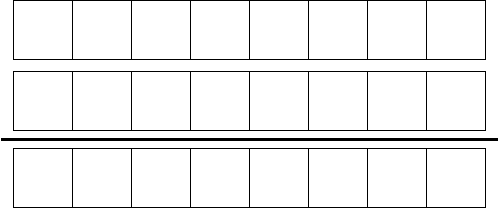
\includegraphics{./systeme_numeration_files/figure-pdf/unnamed-chunk-8-1.pdf}

\end{example}

\leavevmode\vadjust pre{\hypertarget{exm-addition-complement-deux-2}{}}%
\begin{example}[]\label{exm-addition-complement-deux-2}

À l'aide de la complémentation à deux, calculez 75+87.

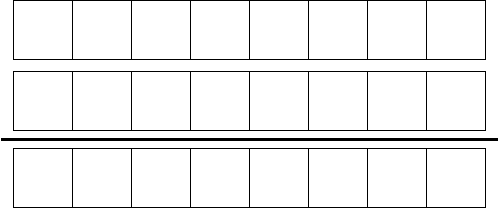
\includegraphics{./systeme_numeration_files/figure-pdf/unnamed-chunk-9-1.pdf}

\end{example}

\leavevmode\vadjust pre{\hypertarget{exm-addition-complement-deux-3}{}}%
\begin{example}[]\label{exm-addition-complement-deux-3}

À l'aide de la complémentation à deux, calculez -64-56.

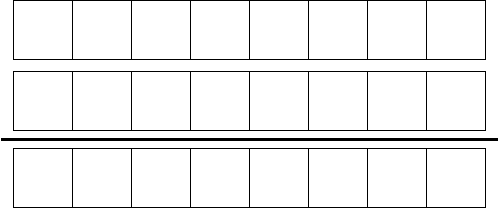
\includegraphics{./systeme_numeration_files/figure-pdf/unnamed-chunk-10-1.pdf}

\end{example}

\leavevmode\vadjust pre{\hypertarget{exm-addition-complement-deux-4}{}}%
\begin{example}[]\label{exm-addition-complement-deux-4}

À l'aide de la complémentation à deux, calculez -78-85.

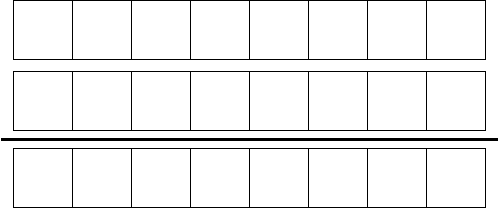
\includegraphics{./systeme_numeration_files/figure-pdf/unnamed-chunk-11-1.pdf}

\end{example}

\hypertarget{addition-de-deux-nombres-de-signes-diffuxe9rents}{%
\subsubsection*{Addition de deux nombres de signes
différents}\label{addition-de-deux-nombres-de-signes-diffuxe9rents}}
\addcontentsline{toc}{subsubsection}{Addition de deux nombres de signes
différents}

\begin{itemize}
\tightlist
\item
  Il n'y a aucun débordement possible (\textbf{POURQUOI?})
\item
  Le résultat peut être positif ou négatif selon la valeur du bit-signe.
\item
  On complémente le résultat si le bit-signe est \texttt{1}.
\end{itemize}

\leavevmode\vadjust pre{\hypertarget{exm-addition-complement-deux-5}{}}%
\begin{example}[]\label{exm-addition-complement-deux-5}

À l'aide de la complémentation à deux, calculez -59-18.

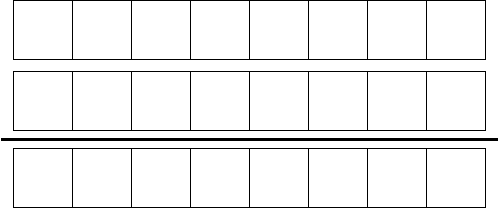
\includegraphics{./systeme_numeration_files/figure-pdf/unnamed-chunk-12-1.pdf}

\end{example}

\leavevmode\vadjust pre{\hypertarget{exm-addition-complement-deux-6}{}}%
\begin{example}[]\label{exm-addition-complement-deux-6}

À l'aide de la complémentation à deux, calculez 18-59.

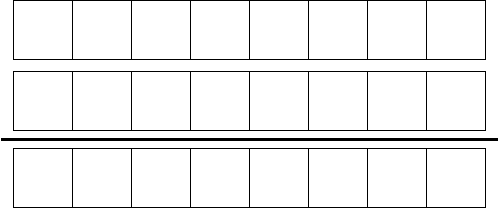
\includegraphics{./systeme_numeration_files/figure-pdf/unnamed-chunk-13-1.pdf}

\end{example}

\hypertarget{opuxe9rateurs-bit-uxe0-bit}{%
\subsection{Opérateurs bit à bit}\label{opuxe9rateurs-bit-uxe0-bit}}

En logique, une opération bit à bit est un calcul manipulant les données
directement au niveau des bits, selon une arithmétique booléenne. Elles
sont utiles dès qu'il s'agit de manipuler les données à bas niveau :
codages, couches basses du réseau (par exemple TCP/IP), cryptographie,
etc.

Les opérations bit à bit courantes comprennent des opérations logiques
bit par bit et des opérations de décalage des bits, vers la droite ou
vers la gauche.

\hypertarget{left-shift}{%
\subsection{LEFT-SHIFT \textless\textless{}}\label{left-shift}}

\hypertarget{right-shift}{%
\subsection{RIGHT-SHIFT \textgreater\textgreater{}}\label{right-shift}}

\hypertarget{compluxe9ment-uxe0-un-muxeame-chose-que-not}{%
\subsection{COMPLÉMENT À UN \textasciitilde{} (MÊME CHOSE QUE
NOT)}\label{compluxe9ment-uxe0-un-muxeame-chose-que-not}}

\hypertarget{repruxe9sentation-des-nombres-en-virgule-flottante}{%
\section{Représentation des nombres en virgule
flottante}\label{repruxe9sentation-des-nombres-en-virgule-flottante}}

\hypertarget{la-norme-ieee754}{%
\subsection{La norme IEEE754}\label{la-norme-ieee754}}

En informatique, l'IEEE 754 est une norme sur l'arithmétique à virgule
flottante mise au point par le \emph{Institute of Electrical and
Electronics Engineers}. Elle est la norme la plus employée actuellement
pour le calcul des nombres à virgule flottante avec les CPU et les FPU.
La norme définit les formats de représentation des nombres à virgule
flottante (signe, mantisse, exposant, nombres dénormalisés) et valeurs
spéciales (infinis et NaN), en même temps qu'un ensemble d'opérations
sur les nombres flottants. Il décrit aussi cinq modes d'arrondi et cinq
exceptions (comprenant les conditions dans lesquelles une exception se
produit, et ce qui se passe dans ce cas).

\hypertarget{format-guxe9nuxe9ral}{%
\subsubsection*{Format général}\label{format-guxe9nuxe9ral}}
\addcontentsline{toc}{subsubsection}{Format général}

Un nombre flottant est formé de trois éléments : la mantisse, l'exposant
et le signe. Le bit de poids fort est le bit de signe : si ce bit est à
1, le nombre est négatif, et s'il est à 0, le nombre est positif. Les
\(e\) bits suivants représentent l'exposant biaisé (sauf valeur
spéciale), et les \(m\) bits suivants (\(m\) bits de poids faible)
représentent la mantisse.

L'exposant peut être positif ou négatif. Cependant, la représentation
habituelle des nombres signés (complément à 2) rendrait la comparaison
entre les nombres flottants un peu plus difficile. Pour régler ce
problème, l'exposant est « biaisé », afin de le stocker sous forme d'un
nombre non signé.

Ce biais est de 2e−1 − 1 (e représente le nombre de bits de l'exposant)
; il s'agit donc d'une valeur constante une fois que le nombre de bits e
est fixé.

\bookmarksetup{startatroot}

\hypertarget{logique}{%
\chapter{Logique}\label{logique}}

\hypertarget{logique-propositionnelle}{%
\section{Logique propositionnelle}\label{logique-propositionnelle}}

\leavevmode\vadjust pre{\hypertarget{def-proposition}{}}%
\begin{definition}[Proposition]\label{def-proposition}

Un énoncé qui est soit vrai, soit faux est appelé une
\textbf{proposition}. La \textbf{valeur de vérité} d'une proposition est
donc \textbf{VRAI} ou \textbf{FAUX}.

En \texttt{Python}, les valeurs de vérités sont données par
\texttt{True} (\textbf{VRAI}) et \texttt{False} (\textbf{FAUX}).

\end{definition}

Un énoncé qui n'est pas une proposition (comme un paradoxe, une phrase
impérative ou interrogative) sera qualifié d'innaceptable.

\leavevmode\vadjust pre{\hypertarget{exm-propositions}{}}%
\begin{example}[]\label{exm-propositions}

Les énoncés suivants sont des propositions:

\begin{itemize}
\tightlist
\item
  Les numéros de téléphones au Canada ont dix chiffres.
\item
  La lune est faite de fromage.
\item
  42 est la réponse à la question portant sur la \emph{vie, l'univers et
  tout ce qui existe}.
\item
  Chaque nombre pair plus grand que 2 peut être exprimé comme la somme
  de deux nombres premiers.
\item
  \(3+7=12\)
\end{itemize}

Les énoncés suivants ne sont \textbf{pas} des propositions:

\begin{itemize}
\tightlist
\item
  Voulez-vous du gâteau?
\item
  La somme de deux carrés.
\item
  \(1+3+5+7+\ldots +2n+1\).
\item
  Va dans ta chambre!
\item
  \(3+x=12\)
\end{itemize}

\end{example}

Nous utilisons une table de vérité pour montrer les valeurs de vérité de
propositions composées.

\hypertarget{la-nuxe9gation}{%
\subsection{La négation}\label{la-nuxe9gation}}

\leavevmode\vadjust pre{\hypertarget{def-negation}{}}%
\begin{definition}[La négation]\label{def-negation}

Soit \(p\) une proposition. L'énoncé:

\begin{quote}
\emph{Il n'est pas vrai que \(p\).}
\end{quote}

est une autre proposition appelée \textbf{négation} de \(p\), qui est
représentée par \(\lnot p\). La proposition \(\lnot p\) se lit \emph{non
\(p\)}. La table de vérité de la négation est donnée ci-dessous.

\begin{longtable}[]{@{}cc@{}}
\toprule()
\(p\) & \(\lnot p\) \\
\midrule()
\endhead
\(\phantom{V}\) & \(\phantom{V}\) \\
\(\phantom{V}\) & \(\phantom{V}\) \\
\bottomrule()
\end{longtable}

En \texttt{Python}, l'opérateur \texttt{not} permet de faire la négation
d'une valeur de vérité.

\hypertarget{negation-python}{}
\begin{Shaded}
\begin{Highlighting}[]
\KeywordTok{def}\NormalTok{ negation(p):}
    \ControlFlowTok{return} \KeywordTok{not}\NormalTok{ p}

\BuiltInTok{print}\NormalTok{(}\StringTok{"p    non\_p"}\NormalTok{)}
\ControlFlowTok{for}\NormalTok{ p }\KeywordTok{in}\NormalTok{ [}\VariableTok{True}\NormalTok{, }\VariableTok{False}\NormalTok{]:}
\NormalTok{    non\_p }\OperatorTok{=}\NormalTok{ negation(p)}
    \BuiltInTok{print}\NormalTok{(p, non\_p)}
\end{Highlighting}
\end{Shaded}

\begin{verbatim}
p    non_p
True False
False True
\end{verbatim}

\end{definition}

\hypertarget{la-conjonction}{%
\subsection{La conjonction}\label{la-conjonction}}

\begin{quote}
Je suis une roche \textbf{ET} je suis une île.
\end{quote}

\leavevmode\vadjust pre{\hypertarget{def-conjonction}{}}%
\begin{definition}[La conjonction]\label{def-conjonction}

Soit \(p\) et \(q\) deux propositions. La proposition \emph{\(p\) et
\(q\)}, notée \(p\wedge q\), est vraie si à la fois \(p\) et \(q\) sont
vraies. Elle est fausse dans tous les autres cas. Cette proposition est
appelée la \textbf{conjonction} de \(p\) et de \(q\). La table de vérité
de la conjonction est donnée ci-dessous.

\begin{longtable}[]{@{}ccc@{}}
\toprule()
\(p\) & \(q\) & \(p \wedge q\) \\
\midrule()
\endhead
\(\phantom{V}\) & \(\phantom{V}\) & \(\phantom{V}\) \\
\(\phantom{V}\) & \(\phantom{V}\) & \(\phantom{V}\) \\
\(\phantom{V}\) & \(\phantom{V}\) & \(\phantom{V}\) \\
\(\phantom{V}\) & \(\phantom{V}\) & \(\phantom{V}\) \\
\bottomrule()
\end{longtable}

En \texttt{Python}, l'opérateur \texttt{and} permet de faire la
conjonction de deux valeurs de vérité.

\hypertarget{conjonction-python}{}
\begin{Shaded}
\begin{Highlighting}[]
\KeywordTok{def}\NormalTok{ conjonction(p, q):}
    \ControlFlowTok{return}\NormalTok{ p }\KeywordTok{and}\NormalTok{ q}

\BuiltInTok{print}\NormalTok{(}\StringTok{"p    q    p\_et\_q"}\NormalTok{)}
\ControlFlowTok{for}\NormalTok{ p }\KeywordTok{in}\NormalTok{ [}\VariableTok{True}\NormalTok{, }\VariableTok{False}\NormalTok{]:}
    \ControlFlowTok{for}\NormalTok{ q }\KeywordTok{in}\NormalTok{ [}\VariableTok{True}\NormalTok{, }\VariableTok{False}\NormalTok{]:}
\NormalTok{        p\_et\_q }\OperatorTok{=}\NormalTok{ conjonction(p, q)}
        \BuiltInTok{print}\NormalTok{(p, q, p\_et\_q)}
\end{Highlighting}
\end{Shaded}

\begin{verbatim}
p    q    p_et_q
True True True
True False False
False True False
False False False
\end{verbatim}

\end{definition}

\hypertarget{la-disjonction}{%
\subsection{La disjonction}\label{la-disjonction}}

\begin{quote}
Elle a étudié très fort \textbf{OU} elle est extrêmement brillante.
\end{quote}

\leavevmode\vadjust pre{\hypertarget{def-disjonction}{}}%
\begin{definition}[La disjonction]\label{def-disjonction}

Soit \(p\) et \(q\) deux propositions. La proposition \emph{\(p\) ou
\(q\)}, notée \(p\vee q\), est fausse si \(p\) et \(q\) sont fausses.
Elle est vraie dans tous les autres cas. Cette proposition est appelée
la \textbf{disjonction} de \(p\) et de \(q\). La table de vérité de la
disjonction est donnée ci-dessous.

\begin{longtable}[]{@{}ccc@{}}
\toprule()
\(p\) & \(q\) & \(p \vee q\) \\
\midrule()
\endhead
\(\phantom{V}\) & \(\phantom{V}\) & \(\phantom{V}\) \\
\(\phantom{V}\) & \(\phantom{V}\) & \(\phantom{V}\) \\
\(\phantom{V}\) & \(\phantom{V}\) & \(\phantom{V}\) \\
\(\phantom{V}\) & \(\phantom{V}\) & \(\phantom{V}\) \\
\bottomrule()
\end{longtable}

En \texttt{Python}, l'opérateur \texttt{or} permet de faire la
disjonction de deux valeurs de vérité.

\hypertarget{disjonction-python}{}
\begin{Shaded}
\begin{Highlighting}[]
\KeywordTok{def}\NormalTok{ disjonction(p, q):}
    \ControlFlowTok{return}\NormalTok{ p }\KeywordTok{or}\NormalTok{ q}

\BuiltInTok{print}\NormalTok{(}\StringTok{"p    q    p\_ou\_q"}\NormalTok{)}
\ControlFlowTok{for}\NormalTok{ p }\KeywordTok{in}\NormalTok{ [}\VariableTok{True}\NormalTok{, }\VariableTok{False}\NormalTok{]:}
    \ControlFlowTok{for}\NormalTok{ q }\KeywordTok{in}\NormalTok{ [}\VariableTok{True}\NormalTok{, }\VariableTok{False}\NormalTok{]:}
\NormalTok{        p\_ou\_q }\OperatorTok{=}\NormalTok{ disjonction(p, q)}
        \BuiltInTok{print}\NormalTok{(p, q, p\_ou\_q)}
\end{Highlighting}
\end{Shaded}

\begin{verbatim}
p    q    p_ou_q
True True True
True False True
False True True
False False False
\end{verbatim}

\end{definition}

\hypertarget{la-disjonction-exclusive}{%
\subsection{La disjonction exclusive}\label{la-disjonction-exclusive}}

\begin{quote}
Prenez \textbf{SOIT} deux Advil \textbf{OU} deux Tylenols.
\end{quote}

\leavevmode\vadjust pre{\hypertarget{def-disjonction-exclusive}{}}%
\begin{definition}[La disjonction
exclusive]\label{def-disjonction-exclusive}

Soit \(p\) et \(q\) deux propositions. La proposition \emph{\(p\) ou
exclusif \(q\)}, notée \(p\oplus q\), est vraie si \(p\) et \(q\) ont
des valeurs de vérité \textbf{différentes}. Elle est fausse dans tous
les autres cas. Cette proposition est appelée la \textbf{disjonction
exclusive} de \(p\) et de \(q\). La table de vérité de la disjonction
exclusive est donnée ci-dessous.

\begin{longtable}[]{@{}ccc@{}}
\toprule()
\(p\) & \(q\) & \(p \oplus q\) \\
\midrule()
\endhead
\(\phantom{V}\) & \(\phantom{V}\) & \(\phantom{V}\) \\
\(\phantom{V}\) & \(\phantom{V}\) & \(\phantom{V}\) \\
\(\phantom{V}\) & \(\phantom{V}\) & \(\phantom{V}\) \\
\(\phantom{V}\) & \(\phantom{V}\) & \(\phantom{V}\) \\
\bottomrule()
\end{longtable}

En \texttt{Python}, il n'existe pas d'opérateur logique pour effectuer
la disjonction exclusive. On peut par contre utiliser l'opérateur bit à
bit \texttt{\^{}} pour faire cette disjonction exclusive.

\end{definition}

\leavevmode\vadjust pre{\hypertarget{exm-disjonction-exclusive-python}{}}%
\begin{example}[]\label{exm-disjonction-exclusive-python}

Utilisez les opérateurs logiques vus précédemment pour construire la
table de vérité de la disjonction exclusive dans \texttt{Python}.

\hypertarget{disjonction-exclusive-python-todo}{}
\begin{Shaded}
\begin{Highlighting}[]
\KeywordTok{def}\NormalTok{ disjonction\_exclusive(p, q):}
    \ControlFlowTok{return} \CommentTok{\#REMPLACEZ MOI\#}

\BuiltInTok{print}\NormalTok{(}\StringTok{"p    q    p\_ou\_exclusif\_q"}\NormalTok{)}
\ControlFlowTok{for}\NormalTok{ p }\KeywordTok{in}\NormalTok{ [}\VariableTok{True}\NormalTok{, }\VariableTok{False}\NormalTok{]:}
    \ControlFlowTok{for}\NormalTok{ q }\KeywordTok{in}\NormalTok{ [}\VariableTok{True}\NormalTok{, }\VariableTok{False}\NormalTok{]:}
\NormalTok{        p\_ou\_exclusif\_q }\OperatorTok{=}\NormalTok{ disjonction\_exclusive(p, q)}
        \BuiltInTok{print}\NormalTok{(p, q, p\_ou\_exclusif\_q)}
\end{Highlighting}
\end{Shaded}

\hypertarget{disjonction-exclusive-python}{}
\begin{verbatim}
p    q    p_ou_exclusif_q
True True False
True False True
False True True
False False False
\end{verbatim}

\end{example}

\begin{tcolorbox}[enhanced jigsaw, opacityback=0, rightrule=.15mm, breakable, toprule=.15mm, colbacktitle=quarto-callout-important-color!10!white, title=\textcolor{quarto-callout-important-color}{\faExclamation}\hspace{0.5em}{Important}, titlerule=0mm, arc=.35mm, colback=white, coltitle=black, colframe=quarto-callout-important-color-frame, bottomtitle=1mm, toptitle=1mm, bottomrule=.15mm, leftrule=.75mm, left=2mm, opacitybacktitle=0.6]

La disjonction exclusive signifie l'un ou l'autre, mais pas les deux.

\end{tcolorbox}

\hypertarget{limplication}{%
\subsection{L'implication}\label{limplication}}

\begin{quote}
\textbf{SI} vous avez 100 à l'examen final, \textbf{ALORS} vous
obtiendrez A dans ce cours.
\end{quote}

\leavevmode\vadjust pre{\hypertarget{def-implication}{}}%
\begin{definition}[L'implication]\label{def-implication}

Soit \(p\) et \(q\) deux propositions. L'\textbf{implication}
\(p\rightarrow q\) est une proposition qui est fausse quand \(p\) est
vraie et que \(q\) est fausse, et qui est vraie dans tous les autres
cas. Dans une implication, \(p\) est appelée l'\textbf{hypothèse} (ou
l'\textbf{antécédent} ou la \textbf{prémisse}) et \(q\), la
\textbf{conclusion} (ou la \textbf{conséquence}). La table de vérité de
l'implication' est donnée ci-dessous.

\begin{longtable}[]{@{}ccc@{}}
\toprule()
\(p\) & \(q\) & \(p \rightarrow q\) \\
\midrule()
\endhead
\(\phantom{V}\) & \(\phantom{V}\) & \(\phantom{V}\) \\
\(\phantom{V}\) & \(\phantom{V}\) & \(\phantom{V}\) \\
\(\phantom{V}\) & \(\phantom{V}\) & \(\phantom{V}\) \\
\(\phantom{V}\) & \(\phantom{V}\) & \(\phantom{V}\) \\
\bottomrule()
\end{longtable}

En \texttt{Python}, il n'existe pas d'opérateur logique pour effectuer
l'implication.

\end{definition}

\leavevmode\vadjust pre{\hypertarget{exm-implication-python}{}}%
\begin{example}[]\label{exm-implication-python}

Utilisez les opérateurs logiques vus précédemment pour construire la
table de vérité de l'implication dans \texttt{Python}.

\hypertarget{implication-python-todo}{}
\begin{Shaded}
\begin{Highlighting}[]
\KeywordTok{def}\NormalTok{ implication(p, q):}
    \ControlFlowTok{return} \CommentTok{\#REMPLACEZ MOI\#}

\BuiltInTok{print}\NormalTok{(}\StringTok{"p    q    p\_implique\_q"}\NormalTok{)}
\ControlFlowTok{for}\NormalTok{ p }\KeywordTok{in}\NormalTok{ [}\VariableTok{True}\NormalTok{, }\VariableTok{False}\NormalTok{]:}
    \ControlFlowTok{for}\NormalTok{ q }\KeywordTok{in}\NormalTok{ [}\VariableTok{True}\NormalTok{, }\VariableTok{False}\NormalTok{]:}
\NormalTok{        p\_implique\_q }\OperatorTok{=}\NormalTok{ implication(p, q)}
        \BuiltInTok{print}\NormalTok{(p, q, p\_implique\_q)}
\end{Highlighting}
\end{Shaded}

\hypertarget{implication-python}{}
\begin{verbatim}
p    q    p_implique_q
True True True
True False False
False True True
False False True
\end{verbatim}

\end{example}

\begin{tcolorbox}[enhanced jigsaw, opacityback=0, rightrule=.15mm, breakable, toprule=.15mm, colbacktitle=quarto-callout-important-color!10!white, title=\textcolor{quarto-callout-important-color}{\faExclamation}\hspace{0.5em}{Important}, titlerule=0mm, arc=.35mm, colback=white, coltitle=black, colframe=quarto-callout-important-color-frame, bottomtitle=1mm, toptitle=1mm, bottomrule=.15mm, leftrule=.75mm, left=2mm, opacitybacktitle=0.6]

Une implication peut être considérée comme un \textbf{contrat} qui
échoue seulement si les conditions du contrat sont respectées mais les
résultats ne sont pas remplis.

\end{tcolorbox}

Comme les implications apparaissent constamment en mathématiques, il
existe une vaste terminologie pour désigner \(p\rightarrow q\). Voici
les modes les plus courants:

\begin{itemize}
\tightlist
\item
  si \(p\) alors \(q\);
\item
  \(p\) implique \(q\);
\item
  \(p\) seulement si \(q\);
\item
  \(p\) est suffisant pour \(q\);
\item
  \(q\) si \(p\);
\item
  \(q\) chaque fois que \(p\);
\item
  \(q\) est nécessaire à \(p\).
\end{itemize}

\hypertarget{la-biconditionnelle}{%
\subsection{La biconditionnelle}\label{la-biconditionnelle}}

\begin{quote}
Il pleut dehors \textbf{SI ET SEULEMENT SI} c'est un jour nuageux.
\end{quote}

\leavevmode\vadjust pre{\hypertarget{def-biconditionnelle}{}}%
\begin{definition}[La biconditionnelle]\label{def-biconditionnelle}

Soit \(p\) et \(q\) deux propositions. La \textbf{biconditionnelle}
\(p\leftrightarrow q\) est une proposition qui est vraie quand \(p\) et
\(q\) ont les mêmes valeurs de vérité et qui est fausse dans les autres
cas. La table de vérité de la biconditionnelle est donnée ci-dessous.

\begin{longtable}[]{@{}ccc@{}}
\toprule()
\(p\) & \(q\) & \(p \leftrightarrow q\) \\
\midrule()
\endhead
\(\phantom{V}\) & \(\phantom{V}\) & \(\phantom{V}\) \\
\(\phantom{V}\) & \(\phantom{V}\) & \(\phantom{V}\) \\
\(\phantom{V}\) & \(\phantom{V}\) & \(\phantom{V}\) \\
\(\phantom{V}\) & \(\phantom{V}\) & \(\phantom{V}\) \\
\bottomrule()
\end{longtable}

En \texttt{Python}, il n'existe pas d'opérateur logique pour effectuer
la biconditionnelle.

\end{definition}

\leavevmode\vadjust pre{\hypertarget{exm-biconditionnelle-python}{}}%
\begin{example}[]\label{exm-biconditionnelle-python}

Utilisez les opérateurs logiques vus précédemment pour construire la
table de vérité de la biconditionnelle dans \texttt{Python}.

\hypertarget{biconditionnelle-python-todo}{}
\begin{Shaded}
\begin{Highlighting}[]
\KeywordTok{def}\NormalTok{ biconditionnelle(p, q):}
    \ControlFlowTok{return} \CommentTok{\#REMPLACEZ MOI\#}

\BuiltInTok{print}\NormalTok{(}\StringTok{"p    q    p\_biconditionnelle\_q"}\NormalTok{)}
\ControlFlowTok{for}\NormalTok{ p }\KeywordTok{in}\NormalTok{ [}\VariableTok{True}\NormalTok{, }\VariableTok{False}\NormalTok{]:}
    \ControlFlowTok{for}\NormalTok{ q }\KeywordTok{in}\NormalTok{ [}\VariableTok{True}\NormalTok{, }\VariableTok{False}\NormalTok{]:}
\NormalTok{        p\_biconditionnelle\_q }\OperatorTok{=}\NormalTok{ biconditionnelle(p, q)}
        \BuiltInTok{print}\NormalTok{(p, q, p\_biconditionnelle\_q)}
\end{Highlighting}
\end{Shaded}

\hypertarget{biconditionnelle-python}{}
\begin{verbatim}
p    q    p_biconditionnelle_q
True True True
True False False
False True False
False False True
\end{verbatim}

\end{example}

\begin{tcolorbox}[enhanced jigsaw, opacityback=0, rightrule=.15mm, breakable, toprule=.15mm, colbacktitle=quarto-callout-important-color!10!white, title=\textcolor{quarto-callout-important-color}{\faExclamation}\hspace{0.5em}{Important}, titlerule=0mm, arc=.35mm, colback=white, coltitle=black, colframe=quarto-callout-important-color-frame, bottomtitle=1mm, toptitle=1mm, bottomrule=.15mm, leftrule=.75mm, left=2mm, opacitybacktitle=0.6]

La biconditionnelle est vraie si les propositions ont la même valeur de
vérité et fausse autrement.

\end{tcolorbox}

Comme les biconditionnelles apparaissent constamment en mathématiques,
il existe une vaste terminologie pour désigner \(p\leftrightarrow q\).
Voici les modes les plus courants:

\begin{itemize}
\tightlist
\item
  \(p\) si et seulement si \(q\);
\item
  \(p\) est nécessaire et suffisante pour \(q\);
\item
  si \(p\) alors \(q\) et réciproquement.
\end{itemize}

\leavevmode\vadjust pre{\hypertarget{def-reciproque-contraposee-inverse}{}}%
\begin{definition}[Réciproque, contraposée et
inverse]\label{def-reciproque-contraposee-inverse}

~

\begin{itemize}
\tightlist
\item
  La \textbf{réciproque} de la proposition \(p\rightarrow q\) est la
  proposition \(q \rightarrow p\).
\item
  La \textbf{contraposée} de la proposition \(p\rightarrow q\) est la
  proposition \(\lnot q \rightarrow \lnot p\).
\item
  L'\textbf{inverse} de la proposition \(p\rightarrow q\) est la
  proposition \(\lnot p \rightarrow \lnot q\).
\end{itemize}

\end{definition}

\hypertarget{uxe9quivalences-propositionnelles}{%
\section{Équivalences
propositionnelles}\label{uxe9quivalences-propositionnelles}}

Une proposition composée est une proposition formée de plusieurs
connecteurs logiques.

\leavevmode\vadjust pre{\hypertarget{def-tautologie-contradiction-contingence}{}}%
\begin{definition}[Tautologie, contradiction et
contingence]\label{def-tautologie-contradiction-contingence}

Une proposition composée qui est toujours vraie, quelle que soit la
valeur de vérité des fonctions qui la compose est appelée une
\textbf{tautologie}. Une proposition composée qui est toujours fausse
est appelée une \textbf{contradiction}. Finalement, une proposition qui
n'est ni une tautologie ni une contradiction est appelée une
\textbf{contingence}.

\end{definition}

\leavevmode\vadjust pre{\hypertarget{exm-tautologie-contradiction}{}}%
\begin{example}[]\label{exm-tautologie-contradiction}

Remplissez la table de vérité suivante et dites si les propositions
composées sont des tautologies, des contradictions ou des contingences.

\begin{longtable}[]{@{}
  >{\centering\arraybackslash}p{(\columnwidth - 6\tabcolsep) * \real{0.2206}}
  >{\centering\arraybackslash}p{(\columnwidth - 6\tabcolsep) * \real{0.2206}}
  >{\centering\arraybackslash}p{(\columnwidth - 6\tabcolsep) * \real{0.2647}}
  >{\centering\arraybackslash}p{(\columnwidth - 6\tabcolsep) * \real{0.2941}}@{}}
\toprule()
\begin{minipage}[b]{\linewidth}\centering
\(p\)
\end{minipage} & \begin{minipage}[b]{\linewidth}\centering
\(q\)
\end{minipage} & \begin{minipage}[b]{\linewidth}\centering
\(p \vee \lnot p\)
\end{minipage} & \begin{minipage}[b]{\linewidth}\centering
\(p \wedge \lnot p\)
\end{minipage} \\
\midrule()
\endhead
\(\phantom{V}\) & \(\phantom{V}\) & \(\phantom{V}\) & \(\phantom{V}\) \\
\(\phantom{V}\) & \(\phantom{V}\) & \(\phantom{V}\) & \(\phantom{V}\) \\
\bottomrule()
\end{longtable}

\end{example}

\leavevmode\vadjust pre{\hypertarget{exm-proposition-compose}{}}%
\begin{example}[]\label{exm-proposition-compose}

Le code ci-dessous révèle la table de vérité de la proposition composée
\((p \wedge q) \vee \lnot q\).

\hypertarget{prop-composee-1}{}
\begin{Shaded}
\begin{Highlighting}[]
\KeywordTok{def}\NormalTok{ conjonction(p, q):}
    \ControlFlowTok{return}\NormalTok{ p }\KeywordTok{and}\NormalTok{ q}

\KeywordTok{def}\NormalTok{ disjonction(p, q):}
    \ControlFlowTok{return}\NormalTok{ p }\KeywordTok{or}\NormalTok{ q}

\BuiltInTok{print}\NormalTok{(}\StringTok{"p    q    a"}\NormalTok{)}
\ControlFlowTok{for}\NormalTok{ p }\KeywordTok{in}\NormalTok{ [}\VariableTok{True}\NormalTok{, }\VariableTok{False}\NormalTok{]:}
    \ControlFlowTok{for}\NormalTok{ q }\KeywordTok{in}\NormalTok{ [}\VariableTok{True}\NormalTok{, }\VariableTok{False}\NormalTok{]:}
\NormalTok{        a }\OperatorTok{=}\NormalTok{ disjonction(conjonction(p, q), }\KeywordTok{not}\NormalTok{ q)}
        \BuiltInTok{print}\NormalTok{(p, q, a)}
\end{Highlighting}
\end{Shaded}

\begin{verbatim}
p    q    a
True True True
True False True
False True False
False False True
\end{verbatim}

De quelle manière pouvez-vous modifier le code précédent pour obtenir la
table de vérité de la proposition composée
\((p \vee \lnot q) \wedge \lnot p\)?

\end{example}

Lorsque vous créez votre table de vérité, il est crucial que vous soyiez
systématique pour vous assurer d'avoir toutes les valeurs de vérité
possibles pour chacune des propositions simples. Chaque proposition a
deux valeurs de vérité possibles, le nombre de lignes de la table
devrait être égal à \(2^n\), où \(n\) est le nombre de propositions.
Vous devriez également considérer de briser vos propositions complexes
en plus petites propositions.

\leavevmode\vadjust pre{\hypertarget{exm-bloc-code}{}}%
\begin{example}[]\label{exm-bloc-code}

L'extrait de code suivant fait intervenir les variables booléennes
\(p\), \(q\) et \(r\). Chacune de ces variables peut prendre les valeurs
\textbf{vrai} ou \textbf{faux}. Pour chaque bloc indiqué, donnez toutes
les valeurs possibles pour \(p\), \(q\) et \(r\) au moment où le bloc
est atteint.

\hypertarget{bloc-code-python}{}
\begin{Shaded}
\begin{Highlighting}[]
\ControlFlowTok{if}\NormalTok{ (p }\KeywordTok{and}\NormalTok{ q):}
    \ControlFlowTok{if}\NormalTok{ r:}
        \CommentTok{\#BLOC 1\#}
    \ControlFlowTok{else}\NormalTok{:}
        \CommentTok{\#BLOC 2\#}
\ControlFlowTok{else}\NormalTok{:}
    \CommentTok{\#BLOC 3\#}
\end{Highlighting}
\end{Shaded}

\begin{longtable}[]{@{}
  >{\centering\arraybackslash}p{(\columnwidth - 10\tabcolsep) * \real{0.1061}}
  >{\centering\arraybackslash}p{(\columnwidth - 10\tabcolsep) * \real{0.1061}}
  >{\centering\arraybackslash}p{(\columnwidth - 10\tabcolsep) * \real{0.1061}}
  >{\centering\arraybackslash}p{(\columnwidth - 10\tabcolsep) * \real{0.2273}}
  >{\centering\arraybackslash}p{(\columnwidth - 10\tabcolsep) * \real{0.2273}}
  >{\centering\arraybackslash}p{(\columnwidth - 10\tabcolsep) * \real{0.2273}}@{}}
\toprule()
\begin{minipage}[b]{\linewidth}\centering
\(p\)
\end{minipage} & \begin{minipage}[b]{\linewidth}\centering
\(q\)
\end{minipage} & \begin{minipage}[b]{\linewidth}\centering
\(r\)
\end{minipage} & \begin{minipage}[b]{\linewidth}\centering
\(\phantom{V}\)
\end{minipage} & \begin{minipage}[b]{\linewidth}\centering
\(\phantom{V}\)
\end{minipage} & \begin{minipage}[b]{\linewidth}\centering
\(\phantom{V}\)
\end{minipage} \\
\midrule()
\endhead
\textbf{V} & \textbf{V} & \textbf{V} & & & \\
\textbf{V} & \textbf{V} & \textbf{F} & & & \\
\textbf{V} & \textbf{F} & \textbf{V} & & & \\
\textbf{V} & \textbf{F} & \textbf{F} & & & \\
\textbf{F} & \textbf{V} & \textbf{V} & & & \\
\textbf{F} & \textbf{V} & \textbf{F} & & & \\
\textbf{F} & \textbf{F} & \textbf{V} & & & \\
\textbf{F} & \textbf{F} & \textbf{F} & & & \\
\bottomrule()
\end{longtable}

\end{example}

\leavevmode\vadjust pre{\hypertarget{def-propositions-equivalentes}{}}%
\begin{definition}[Équivalences de
propositions]\label{def-propositions-equivalentes}

Les propositions \(p\) et \(q\) sont dites \textbf{logiquement
équivalentes} si la proposition \(p \leftrightarrow q\) est une
tautologie. Ainsi, deux propositions sont logiquement équivalentes si
elles ont la même table de vérité, c'est-à-dire la même valeur de vérité
dans tous les cas possibles.

La notation \(p\equiv q\) signifie que \(p\) et \(q\) sont équivalentes.

\end{definition}

\leavevmode\vadjust pre{\hypertarget{exm-proposition-equivalentes-1}{}}%
\begin{example}[]\label{exm-proposition-equivalentes-1}

Vérifiez l'équivalence suivante à l'aide d'une table de vérité. \[
p \rightarrow q \equiv \lnot p \vee q
\]

\begin{longtable}[]{@{}ccccc@{}}
\toprule()
\(p\) & \(q\) & \(\phantom{V}\) & \(\phantom{V}\) & \(\phantom{V}\) \\
\midrule()
\endhead
\textbf{V} & \textbf{V} & & & \\
\textbf{V} & \textbf{F} & & & \\
\textbf{F} & \textbf{V} & & & \\
\textbf{F} & \textbf{F} & & & \\
\bottomrule()
\end{longtable}

\end{example}

\leavevmode\vadjust pre{\hypertarget{exm-proposition-equivalentes-2}{}}%
\begin{example}[]\label{exm-proposition-equivalentes-2}

Vérifiez l'équivalence suivante à l'aide d'une table de vérité. \[
\lnot (p \vee q) \equiv \lnot p \wedge \lnot q
\]

\begin{longtable}[]{@{}
  >{\centering\arraybackslash}p{(\columnwidth - 12\tabcolsep) * \real{0.0787}}
  >{\centering\arraybackslash}p{(\columnwidth - 12\tabcolsep) * \real{0.0787}}
  >{\centering\arraybackslash}p{(\columnwidth - 12\tabcolsep) * \real{0.1685}}
  >{\centering\arraybackslash}p{(\columnwidth - 12\tabcolsep) * \real{0.1685}}
  >{\centering\arraybackslash}p{(\columnwidth - 12\tabcolsep) * \real{0.1685}}
  >{\centering\arraybackslash}p{(\columnwidth - 12\tabcolsep) * \real{0.1685}}
  >{\centering\arraybackslash}p{(\columnwidth - 12\tabcolsep) * \real{0.1685}}@{}}
\toprule()
\begin{minipage}[b]{\linewidth}\centering
\(p\)
\end{minipage} & \begin{minipage}[b]{\linewidth}\centering
\(q\)
\end{minipage} & \begin{minipage}[b]{\linewidth}\centering
\(\phantom{V}\)
\end{minipage} & \begin{minipage}[b]{\linewidth}\centering
\(\phantom{V}\)
\end{minipage} & \begin{minipage}[b]{\linewidth}\centering
\(\phantom{V}\)
\end{minipage} & \begin{minipage}[b]{\linewidth}\centering
\(\phantom{V}\)
\end{minipage} & \begin{minipage}[b]{\linewidth}\centering
\(\phantom{V}\)
\end{minipage} \\
\midrule()
\endhead
\textbf{V} & \textbf{V} & & & & & \\
\textbf{V} & \textbf{F} & & & & & \\
\textbf{F} & \textbf{V} & & & & & \\
\textbf{F} & \textbf{F} & & & & & \\
\bottomrule()
\end{longtable}

\end{example}

Pour gagner du temps, on note les équivalences fréquemment utilisées
dans une table et on leur donne un nom ou un numéro afin d'y faire
référence.

\hypertarget{tbl-equivalences-logiques}{}
\begin{longtable}[]{@{}
  >{\raggedright\arraybackslash}p{(\columnwidth - 4\tabcolsep) * \real{0.1620}}
  >{\raggedright\arraybackslash}p{(\columnwidth - 4\tabcolsep) * \real{0.4155}}
  >{\raggedright\arraybackslash}p{(\columnwidth - 4\tabcolsep) * \real{0.4225}}@{}}
\caption{\label{tbl-equivalences-logiques}Équivalences
logiques}\tabularnewline
\toprule()
\begin{minipage}[b]{\linewidth}\raggedright
\textbf{Nom}
\end{minipage} & \begin{minipage}[b]{\linewidth}\raggedright
\textbf{Équivalence 1}
\end{minipage} & \begin{minipage}[b]{\linewidth}\raggedright
\textbf{Équivalence 2}
\end{minipage} \\
\midrule()
\endfirsthead
\toprule()
\begin{minipage}[b]{\linewidth}\raggedright
\textbf{Nom}
\end{minipage} & \begin{minipage}[b]{\linewidth}\raggedright
\textbf{Équivalence 1}
\end{minipage} & \begin{minipage}[b]{\linewidth}\raggedright
\textbf{Équivalence 2}
\end{minipage} \\
\midrule()
\endhead
\textbf{Identité} & \(p \wedge \mathbf{V} \equiv p\) &
\(p \vee \mathbf{F} \equiv p\) \\
\textbf{Domination} & \(p \vee \mathbf{V} \equiv \mathbf{V}\) &
\(p \wedge \mathbf{F} \equiv \mathbf{F}\) \\
\textbf{Idempotence} & \(p \vee p \equiv p\) & \(p\wedge p \equiv p\) \\
\textbf{Double négation} & \(\lnot (\lnot p) \equiv p\) & \\
\textbf{Commutativité} & \(p\wedge q \equiv q \wedge p\) &
\(p \vee q \equiv q \vee p\) \\
\textbf{Associativité} & \((p \vee q) \vee r \equiv p \vee (q \vee r)\)
& \((p \wedge q) \wedge r \equiv p \wedge (q \wedge r)\) \\
\textbf{Distributivité} &
\(p \vee (q \wedge r) \equiv (p \vee q) \wedge (p \vee r)\) &
\(p\wedge (q \vee r) \equiv (p \wedge q) \vee (p \wedge r)\) \\
\textbf{Lois de De Morgan} &
\(\lnot (p \wedge q) \equiv \lnot p \vee \lnot q\) &
\(\lnot (p \vee q) \equiv \lnot p \wedge \lnot q\) \\
\textbf{Absorption} & \(p \vee (p \wedge q) \equiv p\) &
\(p \wedge (p \vee q) \equiv p\) \\
\textbf{Négation} & \(p \vee \lnot p \equiv \mathbf{V}\) &
\(p \wedge \lnot p \equiv \mathbf{F}\) \\
\bottomrule()
\end{longtable}

\hypertarget{tbl-equivalences-logiques-implications}{}
\begin{longtable}[]{@{}
  >{\raggedright\arraybackslash}p{(\columnwidth - 2\tabcolsep) * \real{0.1333}}
  >{\raggedright\arraybackslash}p{(\columnwidth - 2\tabcolsep) * \real{0.8667}}@{}}
\caption{\label{tbl-equivalences-logiques-implications}Équivalences
logiques (implications)}\tabularnewline
\toprule()
\begin{minipage}[b]{\linewidth}\raggedright
\textbf{Numéro}
\end{minipage} & \begin{minipage}[b]{\linewidth}\raggedright
\textbf{Implication}
\end{minipage} \\
\midrule()
\endfirsthead
\toprule()
\begin{minipage}[b]{\linewidth}\raggedright
\textbf{Numéro}
\end{minipage} & \begin{minipage}[b]{\linewidth}\raggedright
\textbf{Implication}
\end{minipage} \\
\midrule()
\endhead
\textbf{1} & \(p \rightarrow q \equiv \lnot p \vee q\) \\
\textbf{2} & \(p \rightarrow q \equiv \lnot q \rightarrow \lnot p\) \\
\textbf{3} & \(p \vee q \equiv \lnot p \rightarrow q\) \\
\textbf{4} & \(p \wedge q \equiv \lnot(p \rightarrow \lnot q)\) \\
\textbf{5} & \(\lnot(p \rightarrow q) \equiv p \wedge \lnot q\) \\
\textbf{6} &
\((p \rightarrow q)\wedge (p\rightarrow r) \equiv p \rightarrow (q \wedge r)\) \\
\textbf{7} &
\((p \rightarrow r) \wedge (q \rightarrow r) \equiv (p \vee q) \rightarrow r\) \\
\textbf{8} &
\((p\rightarrow q) \vee (p \rightarrow r) \equiv p \rightarrow (q \vee r)\) \\
\textbf{9} &
\((p \rightarrow r) \vee (q \rightarrow r) \equiv (p \wedge q) \rightarrow r\) \\
\bottomrule()
\end{longtable}

\hypertarget{tbl-equivalences-logiques-biconditionnelles}{}
\begin{longtable}[]{@{}
  >{\raggedright\arraybackslash}p{(\columnwidth - 2\tabcolsep) * \real{0.1224}}
  >{\raggedright\arraybackslash}p{(\columnwidth - 2\tabcolsep) * \real{0.8776}}@{}}
\caption{\label{tbl-equivalences-logiques-biconditionnelles}Équivalences
logiques (biconditionnelles)}\tabularnewline
\toprule()
\begin{minipage}[b]{\linewidth}\raggedright
\textbf{Numéro}
\end{minipage} & \begin{minipage}[b]{\linewidth}\raggedright
\textbf{Biconditionnelle}
\end{minipage} \\
\midrule()
\endfirsthead
\toprule()
\begin{minipage}[b]{\linewidth}\raggedright
\textbf{Numéro}
\end{minipage} & \begin{minipage}[b]{\linewidth}\raggedright
\textbf{Biconditionnelle}
\end{minipage} \\
\midrule()
\endhead
\textbf{1} &
\(p \leftrightarrow q \equiv (p\rightarrow q) \wedge (q \rightarrow q)\) \\
\textbf{2} &
\(p \leftrightarrow q \equiv \lnot p \leftrightarrow \lnot q\) \\
\textbf{3} &
\(p \leftrightarrow q \equiv (p \wedge q) \vee (\lnot p \wedge \lnot q)\) \\
\textbf{4} &
\(p \leftrightarrow q \equiv \lnot(p \wedge \lnot q) \wedge \lnot(\lnot p \wedge q )\) \\
\textbf{5} &
\(\lnot(p \leftrightarrow q) \equiv p \leftrightarrow \lnot q\) \\
\bottomrule()
\end{longtable}

\leavevmode\vadjust pre{\hypertarget{exm-proposition-tautologie-deux-manieres}{}}%
\begin{example}[]\label{exm-proposition-tautologie-deux-manieres}

Vérifiez que la proposition \[
\lnot (p \rightarrow q) \rightarrow \lnot q
\] est une tautologie

\begin{enumerate}
\def\labelenumi{\alph{enumi}.}
\item
  à l'aide d'une table de vérité;

  \begin{longtable}[]{@{}
    >{\centering\arraybackslash}p{(\columnwidth - 12\tabcolsep) * \real{0.0787}}
    >{\centering\arraybackslash}p{(\columnwidth - 12\tabcolsep) * \real{0.0787}}
    >{\centering\arraybackslash}p{(\columnwidth - 12\tabcolsep) * \real{0.1685}}
    >{\centering\arraybackslash}p{(\columnwidth - 12\tabcolsep) * \real{0.1685}}
    >{\centering\arraybackslash}p{(\columnwidth - 12\tabcolsep) * \real{0.1685}}
    >{\centering\arraybackslash}p{(\columnwidth - 12\tabcolsep) * \real{0.1685}}
    >{\centering\arraybackslash}p{(\columnwidth - 12\tabcolsep) * \real{0.1685}}@{}}
  \toprule()
  \begin{minipage}[b]{\linewidth}\centering
  \(p\)
  \end{minipage} & \begin{minipage}[b]{\linewidth}\centering
  \(q\)
  \end{minipage} & \begin{minipage}[b]{\linewidth}\centering
  \(\phantom{V}\)
  \end{minipage} & \begin{minipage}[b]{\linewidth}\centering
  \(\phantom{V}\)
  \end{minipage} & \begin{minipage}[b]{\linewidth}\centering
  \(\phantom{V}\)
  \end{minipage} & \begin{minipage}[b]{\linewidth}\centering
  \(\phantom{V}\)
  \end{minipage} & \begin{minipage}[b]{\linewidth}\centering
  \(\phantom{V}\)
  \end{minipage} \\
  \midrule()
  \endhead
  \textbf{V} & \textbf{V} & & & & & \\
  \textbf{V} & \textbf{F} & & & & & \\
  \textbf{F} & \textbf{V} & & & & & \\
  \textbf{F} & \textbf{F} & & & & & \\
  \bottomrule()
  \end{longtable}
\item
  sans l'aide d'une table de vérité, en utilisant les tableaux
  d'équivalences.
\end{enumerate}

\end{example}

\begin{tcolorbox}[enhanced jigsaw, opacityback=0, rightrule=.15mm, breakable, toprule=.15mm, colbacktitle=quarto-callout-important-color!10!white, title=\textcolor{quarto-callout-important-color}{\faExclamation}\hspace{0.5em}{Propositions équivalentes ou non?}, titlerule=0mm, arc=.35mm, colback=white, coltitle=black, colframe=quarto-callout-important-color-frame, bottomtitle=1mm, toptitle=1mm, bottomrule=.15mm, leftrule=.75mm, left=2mm, opacitybacktitle=0.6]

Pour démontrer que les propositions \textbf{ne sont pas} équivalentes,
il suffit de fournir des valeurs de \(p\), \(q\) et \(r\) pour
lesquelles elles diffèrent. Pour démontrer que les propositions sont
équivalentes, on peut procéder de l'une des trois façons suivantes.

\begin{enumerate}
\def\labelenumi{\arabic{enumi}.}
\tightlist
\item
  Fournir leur table de vérité.
\item
  Utiliser la Table~\ref{tbl-equivalences-logiques}, la
  Table~\ref{tbl-equivalences-logiques-implications} ou la
  Table~\ref{tbl-equivalences-logiques-biconditionnelles}.
\item
  Formuler une explication en mots qui montre que les deux propositions
  sont vraies, ou encore que les deux sont fausses, exactement pour les
  mêmes combinaisons de valeur de vérité des variables
  propositionnelles.
\end{enumerate}

\end{tcolorbox}

\hypertarget{pruxe9dicats-et-quantificateurs}{%
\section{Prédicats et
quantificateurs}\label{pruxe9dicats-et-quantificateurs}}

Un énoncé contenant une ou plusieurs variables tel que \[
x<10 \quad \text{ou} \quad x+2=7-y
\] n'est pas une proposition pusique, tant que la valeur de \(x\) ou
\(y\) n'est pas connue, on ne peut dire s'il est vrai ou faux.

\leavevmode\vadjust pre{\hypertarget{def-sujet-predicat}{}}%
\begin{definition}[Terminologie]\label{def-sujet-predicat}

Dans l'énoncé ``\(x<10\)'', \(x\) est le \textbf{sujet}, et ``est
inférieur à 10'' est le \textbf{prédicat}. Notons \(P(x)\) l'énoncé
\(x<10\). On dit que \(P\) est une \textbf{fonction propositionnelle}.

\end{definition}

Une fonction propositionnelle \(P(x)\) prend la valeur vrai ou faux
quand \(x\) est précisé. Par exemple:

\begin{itemize}
\tightlist
\item
  \(P(8)\) est une proposition vraie. On écrira parfois \(P(8)\) est
  vrai (au masculin, en sous-entendant l'énoncé est vrai, ou même
  \(P(8)\equiv \mathbf{V}\)).
\item
  \(P(13)\) est une proposition fausse.
\item
  \(P(\text{Marc-André})\) n'est pas une proposition, car
  \emph{Marc-André} n'est pas une valeur possible pour la variable
  \(x\).
\end{itemize}

L'ensemble des valeurs possibles pour la variable \(x\) est appelé
\textbf{univers du discours}, ou \textbf{domaine} de la fonction \(P\).

\leavevmode\vadjust pre{\hypertarget{def-quantificateurs}{}}%
\begin{definition}[Quantificateurs]\label{def-quantificateurs}

\[
\forall:\ \text{quantificateur universel} \qquad \exists:\ \text{quantificateur existentiel}
\]

\begin{description}
\tightlist
\item[\(\forall\ x\ P(x)\):]
signifie ``Pour toutes les valeurs de \(x\) dans l'univers du discours,
\(P(x)\)''. Ou encore ``Quel que soit \(x\) (dans l'univers du
discours), \(P(x)\)''.
\item[\(\exists\ x\ P(x)\):]
signifie ``Il existe un élément de \(x\) dans l'univers du discours tel
que \(P(x)\)''. Ou encore ``Il y a au moins un \(x\) (dans l'univers du
discours) tel que \(P(x)\)''. Ou encore ``Pour un certain \(x\) (dans
l'univers du discours), \(P(x)\)''.
\end{description}

\textbf{Notation}. Certains auteurs mettent une virgule avant la
fonction propositionnelle, surtout quand celle-ci est composée. Par
exemple: \(\forall\ x,\ (P_1(x)\rightarrow P_2(x) \vee P_3(x))\). Par
ailleurs, si l'ensemble \(U\) n'a pas déjà été identifié, on peut
préciser que la variable \(x\) prendra des valeurs dans l'ensemble \(U\)
ainsi: \(\exists\ x\in U,\ P(x)\).

\end{definition}

Lorsque l'univers du discours est un ensemble fini
\(\{x_1,x_2,\ldots, x_n\}\), on a les équivalences logiques suivantes:

\begin{align*}
\forall\ x\ P(x) &\equiv P(x_1)\wedge P(x_2) \wedge \cdots \wedge P(x_n) \\
\exists\ x\ P(x) &\equiv P(x_1)\vee P(x_2) \vee \cdots \vee P(x_n)
\end{align*}

La quantification universelle \(\forall\ x\ P(x)\) est vraie quand
\(P(x)\) est vraie pour toutes les valeurs de \(x\) dans l'univers du
discours \(U\). Elle est donc fausse s'il existe un \(x\) de \(U\) pour
lequel \(P(x)\) est fausse. Un tel élément est appelé un
\textbf{contre-exemple} de \(\forall\ x\ P(x)\).

La quantification existentielle \(\exists\ x\ P(x)\) est vraie s'il
existe au moins une valeur \(x\) dans l'univers du discours telle que
\(P(x)\) est vraie. Elle est fausse si \(P(x)\) est fausse pour toutes
les valeurs possibles de \(x\).

Ainsi, pour prouver un énoncé de la forme \(\forall\ x\ P(x)\) est vrai,
fournir un exemple de \(x\) tel que \(P(x)\) est vrai ne suffit pas. Il
faut montrer que la proposition \(P(x)\) est vraie pour toutes les
valeurs de \(x\), ce qui peut s'avérer particulièrement
\textbf{difficile lorsque \(U\) est un ensemble infini}. Il en va de
même losqu'on veut prouver qu'un énoncé de la forme \(\exists\ x\ P(x)\)
est faux.

\hypertarget{tbl-prouver-enonce-univers-infini}{}
\begin{longtable}[]{@{}
  >{\raggedright\arraybackslash}p{(\columnwidth - 4\tabcolsep) * \real{0.0948}}
  >{\raggedright\arraybackslash}p{(\columnwidth - 4\tabcolsep) * \real{0.4502}}
  >{\raggedright\arraybackslash}p{(\columnwidth - 4\tabcolsep) * \real{0.4550}}@{}}
\caption{\label{tbl-prouver-enonce-univers-infini}Comment prouver qu'un
énoncé quantifié est vrai ou faux quand l'univers du discours \(U\) est
infini.}\tabularnewline
\toprule()
\begin{minipage}[b]{\linewidth}\raggedright
Pour prouver que
\end{minipage} & \begin{minipage}[b]{\linewidth}\raggedright
est \textbf{vrai}
\end{minipage} & \begin{minipage}[b]{\linewidth}\raggedright
est \textbf{faux}
\end{minipage} \\
\midrule()
\endfirsthead
\toprule()
\begin{minipage}[b]{\linewidth}\raggedright
Pour prouver que
\end{minipage} & \begin{minipage}[b]{\linewidth}\raggedright
est \textbf{vrai}
\end{minipage} & \begin{minipage}[b]{\linewidth}\raggedright
est \textbf{faux}
\end{minipage} \\
\midrule()
\endhead
\(\exists\ x\ P(x)\) & il suffit de fournir \textbf{un exemple}: un
\(x\) de \(U\) tel que \(P(x)\) est vrai. & il faut fournir un argument
général pour montrer que \(P(x)\) est faux quel que soit \(x\) de
\(U\). \\
\(\forall\ x\ P(x)\) & il faut fournir un argument général pour montrer
que \$P(x) est vrai quel que soit \(x\) de \(U\). & il suffit de fournir
un \textbf{contre-exemple}: un \(x\) de \(U\) tel que \(P(x)\) est
faux. \\
\bottomrule()
\end{longtable}

\leavevmode\vadjust pre{\hypertarget{exm-univers-discours-nombres-reels}{}}%
\begin{example}[]\label{exm-univers-discours-nombres-reels}

Si l'univers du discours est l'ensemble des nombres réels et
\begin{align*}
&P(x)\ \text{désigne}\ x\geq 0 \\
&Q(x)\ \text{désigne}\ x\ \text{est un nombre premier} \\
&R(x)\ \text{désigne}\ 3^x+4^x=5^x \\
&S(x)\ \text{désigne}\ x\geq 100
\end{align*} dites si chacun des énoncés suivants est une proposition
vraie, une proposition fausse ou n'est pas une proposition. Donnez un
exemple ou un contre-exemple le cas échéant. Dans le cas contraire,
indiquez qu'un argument général est requis.

\begin{enumerate}
\def\labelenumi{\alph{enumi}.}
\tightlist
\item
  \(\forall\ x\ P(x)\)
\item
  \(\forall\ x\ \lnot P(x)\)
\item
  \(\forall\ x\ P(x^2)\)
\item
  \(\exists\ x\ P(x)\)
\item
  \(\exists\ x\ \lnot P(x)\)
\item
  \(\exists\ x\ Q(x)\)
\item
  \(\exists\ x\ Q(x^2)\)
\item
  \(\forall\ x\ R(x)\)
\item
  \(P(x)\)
\item
  \(\forall\ x\ (S(x)\rightarrow P(x))\)
\item
  \((\forall\ x\ P(x)) \rightarrow (\forall\ x\ S(x))\)
\item
  \(\forall\ x\ S(x+100)\)
\item
  \(\forall\ x\ S(x^2+100)\)
\end{enumerate}

\end{example}

\leavevmode\vadjust pre{\hypertarget{thm-de-morgan-quantificateurs}{}}%
\begin{theorem}[Lois de De Morgan pour les
quantificateurs]\label{thm-de-morgan-quantificateurs}

\[
\lnot \exists\ x\ P(x) \equiv \forall\ x\ \lnot P(x) \qquad \lnot \forall\ x\ P(x) \equiv \exists\ x\ \lnot P(x)
\]

\end{theorem}

\leavevmode\vadjust pre{\hypertarget{exm-univers-etudiants-stjean-repertoire}{}}%
\begin{example}[]\label{exm-univers-etudiants-stjean-repertoire}

Si l'univers du discours est l'ensemble des étudiants du programme
Sciences Informatique et Mathématique (ScIM) et \(M(x)\) désigne
l'énoncé \emph{l'étudiant \(x\) peut modifier les fichiers du répertoire
\(U\)}, traduisez clairement les propositions suivantes à l'aide des
quantificateurs.

\begin{enumerate}
\def\labelenumi{\alph{enumi}.}
\tightlist
\item
  Tous les étudiants de ScIM peuvent modifier les fichiers du répertoire
  \(U\).
\item
  Il est faux que tous les étudiants de ScIM peuvent modifier les
  fichiers du répertoire \(U\).
\item
  Au moins un étudiant de ScIM peut modifier les fichiers du répertoire
  \(U\).
\item
  Il est faux qu'au moins un étudiant de ScIM peut modifier les fichiers
  du répertoire \(U\).
\item
  Aucun étudiant de ScIM ne peut modifier les fichiers du répertoire
  \(U\).
\item
  Au moins un étudiant de ScIM ne peut pas modifier les fichiers du
  répertoire \(U\).
\end{enumerate}

De plus, déterminez les propositions ci-dessus qui sont équivalentes.

\end{example}

\leavevmode\vadjust pre{\hypertarget{exm-univers-billes-rouges-bleues}{}}%
\begin{example}[]\label{exm-univers-billes-rouges-bleues}

Si l'univers du discours est l'ensemble des billes contenues dans un
bol, et si

\begin{itemize}
\tightlist
\item
  \(G(x)\) désigne \emph{la bille \(x\) est grosse}
\item
  \(J(x)\) désigne \emph{la bille \(x\) est jaune}
\item
  \(R(x)\) désigne \emph{la bille \(x\) est rouge}
\item
  \(B(x)\) désigne \emph{la bille \(x\) est bleue}
\end{itemize}

traduisez clairement les propositions suivantes en prenant soin de bien
formuler les phrases.

\begin{enumerate}
\def\labelenumi{\alph{enumi}.}
\tightlist
\item
  \(\forall\ x\ (R(x) \vee J(x))\)
\item
  \((\forall\ x\ R(x)) \vee (\forall\ x\ J(x))\)
\item
  Les propositions a. et b. sont-elles équivalentes?
\item
  \(\exists\ x\ B(x)\)
\item
  \(\lnot(\exists\ x\ B(x))\)
\item
  Utilisez le quantificateur universel \(\forall\) pour écrire une
  proposition équivalente à la précédente.
\item
  \(\lnot(\forall\ x\ R(x))\)
\item
  Utilisez le quantificateur existentiel \(\exists\) pour écrire une
  proposition équivalente à la précédente.
\item
  \(\forall\ x\ (G(x) \rightarrow B(x))\)
\item
  \(\exists\ x\ (G(x) \wedge B(x))\)
\item
  \((\exists\ x\ G(x)) \wedge (\exists\ x\ B(x))\)
\item
  Les deux propositions précédentes sont-elles équivalentes?
\item
  Les deux propositions suivantes sont-elles équivalentes? \[
  (\exists\ x\ R(x)) \vee (\exists\ x\ J(x)) \qquad \text{et} \qquad \exists\ x\ (R(x) \vee J(x))
  \]
\item
  Les deux propositions suivantes sont-elles équivalentes? \[
  (\forall\ x\ R(x)) \wedge (\forall\ x\ G(x)) \qquad \text{et} \qquad \forall\ x\ (R(x) \wedge G(x))
  \]
\end{enumerate}

\end{example}

\hypertarget{opuxe9rations-bit-uxe0-bit}{%
\section{Opérations bit à bit}\label{opuxe9rations-bit-uxe0-bit}}

\hypertarget{probluxe8mes-de-logique}{%
\section{Problèmes de logique}\label{probluxe8mes-de-logique}}

Les problèmes suivants se déroulent sur une île imaginaire où tous les
habitants sont soit des \textbf{chevaliers}, qui disent toujours la
vérité, soit des \textbf{fripons}, qui mentent toujours. Ces énigmes
implique un visiteur qui rencontre un petit groupe d'habitants de l'île.
La plupart du temps, le but du visiteur est de \emph{déduire} les types
des habitants à partir de leurs énoncés.

Voici un exemple type de problème possible.

\begin{tcolorbox}[enhanced jigsaw, opacityback=0, rightrule=.15mm, colback=white, breakable, colframe=quarto-callout-color-frame, leftrule=.75mm, bottomrule=.15mm, arc=.35mm, toprule=.15mm, left=2mm]

\textbf{Déduisez!}\vspace{2mm}

En vous promenant sur l'île, vous rencontrez trois habitants gardant un
pont. Pour passer, vous devez déduire le type de chaque habitant. Chaque
individu dit un seul énoncé:

\begin{itemize}
\tightlist
\item
  Individu A: Si je suis un fripon, alors il y a exactement deux
  chevaliers ici.
\item
  Individu B: L'individu A ment.
\item
  Individu C: Soit nous sommes tous des fripons ou alors au moins l'un
  d'entre nous est un chevalier.
\end{itemize}

Quels sont les types des trois individus?

\end{tcolorbox}

\hypertarget{stratuxe9gies}{%
\subsection*{Stratégies}\label{stratuxe9gies}}
\addcontentsline{toc}{subsection}{Stratégies}

Voici quelques stratégies que vous pouvez utiliser pour résoudre ce
genre de problème:

\begin{itemize}
\tightlist
\item
  Commencez en supposant qu'un individu est d'un certain type. Soyez
  stratégique avec votre supposition, tentez de résoudre un énoncé
  \textbf{ET}.

  \begin{itemize}
  \tightlist
  \item
    Si un individu dit \textbf{ET}, supposez qu'il est un chevalier;
  \item
    Si un individu dit \textbf{OU}, supposez qu'il est un fripon;
  \item
    Si un individu dit \textbf{SI/ALORS}, supposez qu'il est un fripon;
  \item
    Si un individu dit \textbf{SI ET SEULEMENT SI}, attendez de
    connaître la valeur de vérité de leur énoncé avant de faire une
    supposition.
  \end{itemize}
\item
  Lorsqu'un individu est un chevalier, vous pouvez continuer leur
  énoncé.
\item
  Lorsqu'un individu est un fripon, vous pouvez continuer la négation de
  leur énoncé.

  \begin{itemize}
  \tightlist
  \item
    Partie 1 \textbf{ET} Partie 2 \(\rightarrow\) \textbf{NON} Partie 1
    \textbf{OU} \textbf{NON} Partie 2
  \item
    Partie 1 \textbf{OU} Partie 2 \(\rightarrow\) \textbf{NON} Partie 1
    \textbf{ET} \textbf{NON} Partie 2
  \item
    \textbf{SI} Partie 1, alors Partie 2 \(\rightarrow\) Partie 1
    \textbf{ET} \textbf{NON} Partie 2
  \end{itemize}
\item
  Soyez prudents avec les \emph{si et seulement si}

  \begin{itemize}
  \tightlist
  \item
    Lorsqu'un \emph{si et seulement si} est \texttt{VRAI}, alors les
    deux parties ont la \textbf{même} valeur de vérité.
  \item
    Lorsqu'un \emph{si et seulement si} est \texttt{FAUX}, alors les
    deux parties ont des valeurs de vérités \textbf{différentes}.
  \end{itemize}
\item
  Lorsque vous avez prouvé l'identité d'un individu, vous pouvez
  utiliser cette information partout dans le reste de l'énigme.
\item
  Si vous avez suffisament d'information pour confirmer que l'énoncé
  d'un individu est \texttt{VRAI}, alors ils doivent être un chevalier.
\item
  Si vous avez suffisament d'information pour confirmer que l'énoncé
  d'un individu est \texttt{FAUX}, alors ils doivent être un fripon.
\end{itemize}

\hypertarget{trois-uxe9noncuxe9s-diffuxe9rents}{%
\subsection{Trois énoncés
différents}\label{trois-uxe9noncuxe9s-diffuxe9rents}}

Nous pouvons, dans la plupart des problèmes, regrouper les énoncés des
habitants de l'île en trois formes distinctes.

\hypertarget{accusations-et-affirmations}{%
\subsubsection{Accusations et
affirmations}\label{accusations-et-affirmations}}

Dans une accusation, un habitant \emph{A} dit par exemple \emph{B est un
fripon} ou un énoncé équivalent comme \emph{B ment toujours}. Dans une
affirmation, l'habitant \emph{A} dit par exemple \emph{B est un
chevalier} ou alors \emph{B dit toujours la vérité}.

\leavevmode\vadjust pre{\hypertarget{exm-accusation-different-types}{}}%
\begin{example}[]\label{exm-accusation-different-types}

Que pouvez-vous conclure si \emph{A} et \emph{B} sont reliés par une
\textbf{accusation}?

\end{example}

\leavevmode\vadjust pre{\hypertarget{exm-accusation-different-types}{}}%
\begin{example}[]\label{exm-accusation-different-types}

Que pouvez-vous conclure si \emph{A} et \emph{B} sont reliés par une
\textbf{affirmation}?

\end{example}

\hypertarget{conjonctions-de-fripons}{%
\subsubsection{Conjonctions de fripons}\label{conjonctions-de-fripons}}

Un exemple de conjonction de fripons est lorsque \emph{A} dit que
\emph{B est un chevalier ou je suis un fripon}, ou alors \emph{C est un
fripon et je suis un fripon}

\leavevmode\vadjust pre{\hypertarget{exm-conjonction-de-fripons-ou}{}}%
\begin{example}[]\label{exm-conjonction-de-fripons-ou}

Que pouvez-vous conclure si \emph{A} et \emph{B} sont reliés par
\textbf{ou je suis un fripon}?

\end{example}

\leavevmode\vadjust pre{\hypertarget{exm-conjonction-de-fripons-et}{}}%
\begin{example}[]\label{exm-conjonction-de-fripons-et}

Que pouvez-vous conclure si \emph{A} et \emph{B} sont reliés par
\textbf{et je suis un fripon}?

\end{example}

\hypertarget{uxe9noncuxe9s-de-diffuxe9rences-ou-de-similarituxe9s}{%
\subsubsection{Énoncés de différences ou de
similarités}\label{uxe9noncuxe9s-de-diffuxe9rences-ou-de-similarituxe9s}}

Parfois un habitant \emph{A} dira \emph{B est de mon type} ou peut-être
\emph{C n'est pas de mon type}.

\leavevmode\vadjust pre{\hypertarget{exm-similarite-fripons}{}}%
\begin{example}[]\label{exm-similarite-fripons}

Que pouvez-vous conclure si \emph{A} dit que \emph{B est de son type}?

\end{example}

\leavevmode\vadjust pre{\hypertarget{exm-difference-fripons}{}}%
\begin{example}[]\label{exm-difference-fripons}

Que pouvez-vous conclure si \emph{A} dit que \emph{C n'est pas de son
type}?

\end{example}

Il est intéressant de comparer ces énoncés avec ceux d'accusations et
d'affirmations. Ces deux types d'énoncés sont réciproques en quelque
sorte. Lorsqu'un habitant dit directement de quel type est un autre
habitant (dans une accusation ou une affirmation), tout ce qu'on apprend
c'est que la source et la cible sont similaires ou différents, sans
apprendre leur type. Par contre, lorsqu'un habitant dit un énoncé par
rapport aux similitudes ou aux différences, nous apprenons exactement de
quel type la cible est, sans apprendre si elle est similaire ou
différente de la source.

\leavevmode\vadjust pre{\hypertarget{exm-chevaliers-et-fripons-1}{}}%
\begin{example}[]\label{exm-chevaliers-et-fripons-1}

Vous rencontrez trois habitants de l'île.

\begin{itemize}
\tightlist
\item
  A dit: B ne ment jamais.
\item
  A dit: C est un chevalier ou je suis un fripon.
\end{itemize}

\end{example}

\leavevmode\vadjust pre{\hypertarget{exm-chevaliers-et-fripons-2}{}}%
\begin{example}[]\label{exm-chevaliers-et-fripons-2}

Vous rencontrez trois habitants de l'île.

\begin{itemize}
\tightlist
\item
  A dit: B ment toujours.
\item
  B dit: A n'est pas de mon type.
\end{itemize}

\end{example}

\bookmarksetup{startatroot}

\hypertarget{thuxe9orie-des-ensembles}{%
\chapter{Théorie des ensembles}\label{thuxe9orie-des-ensembles}}

\hypertarget{notions-de-base-sur-les-ensembles}{%
\section{Notions de base sur les
ensembles}\label{notions-de-base-sur-les-ensembles}}

\leavevmode\vadjust pre{\hypertarget{def-ensemble-element}{}}%
\begin{definition}[Ensemble, élément]\label{def-ensemble-element}

Un \textbf{ensemble} est un collection non ordonnée d'objets. Les objets
sont appelés \textbf{éléments} de l'ensemble et on dit qu'ils
appartiennent à l'ensemble.

Notation : \(x\in F\) signifie que \(x\) est un élément de l'ensemble
\(F\). On dit aussi que \(x\) appartient à l'ensemble \(F\).

\end{definition}

\leavevmode\vadjust pre{\hypertarget{def-ensemble-fini-infini-cardinalite}{}}%
\begin{definition}[Ensemble fini ou infini,
cardinalité]\label{def-ensemble-fini-infini-cardinalite}

Soit \(A\) un ensemble composé de \(n\) éléments distincts. On dit que
\(A\) est un \textbf{ensemble fini} de \textbf{cardinalité} \(n\) et on
note \(|A|=n\). Un ensemble est dit \textbf{infini} s'il n'est pas fini.

\end{definition}

\leavevmode\vadjust pre{\hypertarget{exm-ensemble-simple}{}}%
\begin{example}[]\label{exm-ensemble-simple}

Soit l'ensemble \(F=\set{2,\pi,7}\). Utilisez les symboles introduits
pour traduire les énoncés suivants: l'ensemble \(F\) contient 3
éléments, \(\pi\) appartient à \(F\), 5 n'appartient pas à \(F\).

\end{example}

On peut décrire un ensemble \textbf{en extension} (on énumère ses
éléments que l'on place entre accolades) \[
A=\set{5,7,9,11} \qquad B=\set{1,8,27,64}
\] ou en \textbf{compréhension}, comme ceci: \[
A=\set{x\in\mathbb{N}\mid (x\ \text{est impair}) \wedge (5\leq x \leq 11)} \qquad
B=\set{x\in\mathbb{N}\mid (x \leq 64) \wedge (\exists\ y\in \mathbb{N},\ y^3=x)}
\]

Pour créer un ensemble dans \texttt{Python}, nous allons utiliser une
paire d'accolades \texttt{\{} \texttt{\}} et placer les différents
éléments de notre ensemble entre ces accolades en les séparant avec une
virgule. De plus, nous pouvons vérifier si un élément appartient à
l'ensemble en utilisant la commande \texttt{in}.

\hypertarget{ensemble-accolades}{}
\begin{Shaded}
\begin{Highlighting}[]
\NormalTok{A}\OperatorTok{=}\NormalTok{\{}\OperatorTok{{-}}\DecValTok{2}\NormalTok{,}\DecValTok{0}\NormalTok{,}\DecValTok{1}\NormalTok{,}\DecValTok{4}\NormalTok{\}}
\BuiltInTok{print}\NormalTok{(A, }\DecValTok{1} \KeywordTok{in}\NormalTok{ A, }\DecValTok{5} \KeywordTok{in}\NormalTok{ A)}
\end{Highlighting}
\end{Shaded}

\begin{verbatim}
{0, 1, 4, -2} True False
\end{verbatim}

Pour calculer la cardinalité d'un ensemble dans \texttt{Python}, vous
utilisez la fonction \texttt{len()}. En \texttt{Python}, il faut être
prudent si on souhaite utiliser l'ensemble vide, \(\emptyset\). Si vous
utilisez \texttt{\{\}} pour décrire l'ensemble vide, \texttt{Python} va
plutôt l'interpréter comme un \emph{dictionnaire} vide. Vous devez
plutôt utiliser la fonction \texttt{set()}.

\hypertarget{cardinalite-python}{}
\begin{Shaded}
\begin{Highlighting}[]
\NormalTok{A }\OperatorTok{=}\NormalTok{ \{}\DecValTok{2}\NormalTok{,}\DecValTok{3}\NormalTok{,}\DecValTok{5}\NormalTok{,}\DecValTok{8}\NormalTok{\}}
\NormalTok{B }\OperatorTok{=} \BuiltInTok{set}\NormalTok{()}
\NormalTok{C }\OperatorTok{=}\NormalTok{ \{}\DecValTok{0}\NormalTok{\}}
\BuiltInTok{print}\NormalTok{(}\BuiltInTok{len}\NormalTok{(A), }\BuiltInTok{len}\NormalTok{(B), }\BuiltInTok{len}\NormalTok{(C))}
\end{Highlighting}
\end{Shaded}

\begin{verbatim}
4 0 1
\end{verbatim}

\hypertarget{ensembles-de-nombres-mathbbn-mathbbz-mathbbq-mathbbr}{%
\section{\texorpdfstring{Ensembles de nombres \(\mathbb{N}\),
\(\mathbb{Z}\), \(\mathbb{Q}\),
\(\mathbb{R}\)}{Ensembles de nombres \textbackslash mathbb\{N\}, \textbackslash mathbb\{Z\}, \textbackslash mathbb\{Q\}, \textbackslash mathbb\{R\}}}\label{ensembles-de-nombres-mathbbn-mathbbz-mathbbq-mathbbr}}

Nous détaillerons dans la Table~\ref{tbl-ensembles-nombres-usuels}, les
ensembles de nombres les plus communs.

\hypertarget{tbl-ensembles-nombres-usuels}{}
\begin{longtable}[]{@{}
  >{\raggedright\arraybackslash}p{(\columnwidth - 2\tabcolsep) * \real{0.5695}}
  >{\raggedright\arraybackslash}p{(\columnwidth - 2\tabcolsep) * \real{0.4305}}@{}}
\caption{\label{tbl-ensembles-nombres-usuels}Ensembles de nombres
usuels.}\tabularnewline
\toprule()
\begin{minipage}[b]{\linewidth}\raggedright
\textbf{Ensemble}
\end{minipage} & \begin{minipage}[b]{\linewidth}\raggedright
\textbf{Description}
\end{minipage} \\
\midrule()
\endfirsthead
\toprule()
\begin{minipage}[b]{\linewidth}\raggedright
\textbf{Ensemble}
\end{minipage} & \begin{minipage}[b]{\linewidth}\raggedright
\textbf{Description}
\end{minipage} \\
\midrule()
\endhead
\(\emptyset = \set{\phantom{1}}\) & Ensemble vide (ne contient aucun
élément \(\mid\emptyset\mid=0\)) \\
\(\mathbb{N}=\set{0,1,2,3,\ldots}\) & Ensemble des nombres naturels \\
\(\mathbb{N^*}=\set{1,2,3,\ldots}\) & Ensemble des nombres naturels
strictement positifs \\
\(\mathbb{Z}=\set{\ldots,-2,-1,0,1,2,\ldots}\) & Ensemble des nombres
entiers \\
\(\mathbb{Z^*}=\set{\ldots,-2,-1,1,2,\ldots}\) & Ensemble des entiers
non nuls \\
\(\mathbb{Q}=\set{\frac{p}{q}\mid p\in\mathbb{Z},q\in\mathbb{Z}\ \text{et}\ q\neq 0}\)
& Ensemble des nombres rationnels \\
\(\mathbb{R}\) & Ensemble des nombres réels \\
\(\mathbb{R^+}=\set{x\in\mathbb{R}\mid x\geq 0}\) & Ensemble des nombres
réels positifs \\
\(\mathbb{C}=\set{a+bi\mid a\in \mathbb{R}\ \text{et}\ b\in\mathbb{R}}\)
avec \(i^2=-1\) & Ensemble des nombres complexes \\
\bottomrule()
\end{longtable}

\leavevmode\vadjust pre{\hypertarget{exm-ensembles-creation-par-comprehension}{}}%
\begin{example}[]\label{exm-ensembles-creation-par-comprehension}

Établissez un lien entre les ensembles décrits par compréhension aux
parties a. à f.~avec le même ensemble décrit par extension aux parties 1
à 6.

\begin{enumerate}
\def\labelenumi{\alph{enumi}.}
\tightlist
\item
  \(\set{x\in\mathbb{Z}\mid x^2=1}\)
\item
  \(\set{x\in\mathbb{Z}\mid x^3=1}\)
\item
  \(\set{x\in\mathbb{Z}\mid |x|\leq 2}\)
\item
  \(\set{x\in\mathbb{Z}\mid x^2 \leq 4}\)
\item
  \(\set{x\in\mathbb{Z}\mid x<|x|}\)
\item
  \(\set{x\in\mathbb{Z}\mid (x+1)^2=x^2+2x+1}\)
\end{enumerate}

\begin{enumerate}
\def\labelenumi{\arabic{enumi}.}
\tightlist
\item
  \(\set{-1,0,1}\)
\item
  \(\set{\ldots,-3,-2,-1,0,1,2,3,\ldots}\)
\item
  \(\set{1}\)
\item
  \(\set{\ldots,-3,-2,-1}\)
\item
  \(\set{-1,1}\)
\item
  \(\set{-2,-1,0,1,2}\)
\end{enumerate}

\end{example}

\begin{tcolorbox}[enhanced jigsaw, opacityback=0, rightrule=.15mm, breakable, toprule=.15mm, colbacktitle=quarto-callout-note-color!10!white, title=\textcolor{quarto-callout-note-color}{\faInfo}\hspace{0.5em}{Note}, titlerule=0mm, arc=.35mm, colback=white, coltitle=black, colframe=quarto-callout-note-color-frame, bottomtitle=1mm, toptitle=1mm, bottomrule=.15mm, leftrule=.75mm, left=2mm, opacitybacktitle=0.6]

Lorsqu'il y a trop d'éléments dans un ensemble pour être en mesure de
tous les écrire, nous utilisons souvent les trois-points (\(\ldots\))
lorsque la suite d'éléments est claire. Par exemple, nous avons: \[
\mathbb{Z}=\set{\ldots,-3,-2,-1,0,1,2,3,\ldots}
\]

\end{tcolorbox}

En \texttt{Python}, si vous avez un ensemble décrit par compréhension,
il est particulièrement facile de le créer avec une
\texttt{compréhension\ de\ liste}. L'idée est simple: simplifier le code
pour le rendre plus lisible et donc plus rapide à écrire et plus simple
à maintenir. La syntaxe est la suivante:

\begin{verbatim}
new_list = [function(item) for item in list if condition(item)]
new_list = {function(item) for item in list if condition(item)}
\end{verbatim}

Par exemple, si vous voulez créer l'ensemble
\(\set{x^3\mid 0\leq x < 10}\), nous pouvons le faire en \texttt{Python}
de la manière suivante:

\hypertarget{comprehension-de-liste}{}
\begin{Shaded}
\begin{Highlighting}[]
\NormalTok{ensemble }\OperatorTok{=}\NormalTok{ \{x}\OperatorTok{**}\DecValTok{3} \ControlFlowTok{for}\NormalTok{ x }\KeywordTok{in} \BuiltInTok{range}\NormalTok{(}\DecValTok{10}\NormalTok{)\}}
\NormalTok{liste }\OperatorTok{=}\NormalTok{ [x}\OperatorTok{**}\DecValTok{3} \ControlFlowTok{for}\NormalTok{ x }\KeywordTok{in} \BuiltInTok{range}\NormalTok{(}\DecValTok{10}\NormalTok{)]}
\BuiltInTok{print}\NormalTok{(ensemble, liste)}
\end{Highlighting}
\end{Shaded}

\begin{verbatim}
{0, 1, 64, 512, 8, 343, 216, 729, 27, 125} [0, 1, 8, 27, 64, 125, 216, 343, 512, 729]
\end{verbatim}

\begin{tcolorbox}[enhanced jigsaw, opacityback=0, rightrule=.15mm, breakable, toprule=.15mm, colbacktitle=quarto-callout-note-color!10!white, title=\textcolor{quarto-callout-note-color}{\faInfo}\hspace{0.5em}{Note}, titlerule=0mm, arc=.35mm, colback=white, coltitle=black, colframe=quarto-callout-note-color-frame, bottomtitle=1mm, toptitle=1mm, bottomrule=.15mm, leftrule=.75mm, left=2mm, opacitybacktitle=0.6]

Remarquez que dans l'ensemble, les éléments ne sont pas ordonnés, tandis
qu'ils le sont dans la liste.

\end{tcolorbox}

\leavevmode\vadjust pre{\hypertarget{def-egalite-ensembles}{}}%
\begin{definition}[Égalité d'ensembles]\label{def-egalite-ensembles}

Deux ensembles sont dits égaux si et seulement s'ils contiennent
exactement les mêmes éléments. \[
A=B \leftrightarrow \forall\ x\ (x\in A \leftrightarrow x\in B)
\]

\end{definition}

\leavevmode\vadjust pre{\hypertarget{exm-ensembles-egaux-oui-non}{}}%
\begin{example}[]\label{exm-ensembles-egaux-oui-non}

Les ensembles suivants sont-ils égaux? \begin{align*}
\set{1,3,5} &\stackrel{?}{=} \set{3,5,1} \\
\set{1,3,5} &\stackrel{?}{=} \set{\set{1},\set{3},\set{5}}
\end{align*}

\end{example}

\leavevmode\vadjust pre{\hypertarget{def-sous-ensemble}{}}%
\begin{definition}[Sous-ensemble]\label{def-sous-ensemble}

L'ensemble \(A\) est \textbf{sous-ensemble} de l'ensemble \(B\) si et
seulement si tous les éléments de \(A\) sont aussi des éléments de
\(B\): \[
A \subseteq B \leftrightarrow \forall\ x\ (x\in A \rightarrow x\in B)
\] L'ensemble \(A\) est \textbf{sous-ensemble strict (ou propre)} de
l'ensemble \(B\) si et seulement si tous les éléments de \(A\) sont
aussi des éléments de \(B\) et \(A\) n'est pas égal à \(B\): \[
A \subset B \leftrightarrow A\subseteq B \wedge\ A\neq B
\]

\end{definition}

\leavevmode\vadjust pre{\hypertarget{exm-sous-ensembles-verification}{}}%
\begin{example}[]\label{exm-sous-ensembles-verification}

Convainquez-vous des affirmations suivantes. \begin{align*}
\set{1,2} &\subseteq \set{1,2,3,4,5} \\
\set{1,2} &\subset \set{1,2,3,4,5} \\
\set{2k\mid k\in\mathbb{N}} &= \set{0,2,4,6,\ldots}\subset\mathbb{N}
\end{align*}

\end{example}

\hypertarget{tbl-notation-theorie-ensembles}{}
\begin{longtable}[]{@{}
  >{\raggedright\arraybackslash}p{(\columnwidth - 2\tabcolsep) * \real{0.0927}}
  >{\raggedright\arraybackslash}p{(\columnwidth - 2\tabcolsep) * \real{0.9073}}@{}}
\caption{\label{tbl-notation-theorie-ensembles}Notation de la théorie
des ensembles.}\tabularnewline
\toprule()
\begin{minipage}[b]{\linewidth}\raggedright
\textbf{Notation}
\end{minipage} & \begin{minipage}[b]{\linewidth}\raggedright
\textbf{Description}
\end{minipage} \\
\midrule()
\endfirsthead
\toprule()
\begin{minipage}[b]{\linewidth}\raggedright
\textbf{Notation}
\end{minipage} & \begin{minipage}[b]{\linewidth}\raggedright
\textbf{Description}
\end{minipage} \\
\midrule()
\endhead
\(\in\) & \(2\in\set{1,2,3}\) indique que 2 est \textbf{un élément de}
l'ensemble \(\set{1,2,3}\). \\
\(\not\in\) & \(4\not\in\set{1,2,3}\) indique que 4 \textbf{n'est pas un
élément de} l'ensemble \(\set{1,2,3}\). \\
\(\subseteq\) & \(A\subseteq B\) indique que \(A\) est un
\textbf{sous-ensemble} de \(B\): chaque élément de \(A\) est aussi un
élément de \(B\). \\
\(\subset\) & \(A\subset B\) indique que \(A\) est un
\textbf{sous-ensemble propre} de \(B\): chaque élément de \(A\) est
aussi un élément de \(B\), mais \(A\neq B\). \\
\bottomrule()
\end{longtable}

\leavevmode\vadjust pre{\hypertarget{thm-sous-ensemble-vide}{}}%
\begin{theorem}[]\label{thm-sous-ensemble-vide}

Pour tout ensemble \(A\), on a :

\begin{enumerate}
\def\labelenumi{\arabic{enumi}.}
\tightlist
\item
  \(\emptyset\subseteq A\)
\item
  \(A\subseteq A\)
\end{enumerate}

\end{theorem}

\leavevmode\vadjust pre{\hypertarget{thm-sous-ensemble-egalite-ensemble}{}}%
\begin{theorem}[]\label{thm-sous-ensemble-egalite-ensemble}

\(A=B\) si et seulement si \(A\subseteq B\) et \(B\subseteq A\).

\end{theorem}

En \texttt{Python}, nous pouvons utiliser la fonction \texttt{issubset}
pour vérifier qu'un ensemble est sous-ensemble d'un autre.

\hypertarget{sous-ensemble-verification}{}
\begin{Shaded}
\begin{Highlighting}[]
\NormalTok{A }\OperatorTok{=}\NormalTok{ \{}\DecValTok{2}\NormalTok{,}\DecValTok{4}\NormalTok{,}\DecValTok{6}\NormalTok{,}\DecValTok{8}\NormalTok{,}\DecValTok{10}\NormalTok{,}\DecValTok{12}\NormalTok{\}}
\NormalTok{B }\OperatorTok{=}\NormalTok{ \{}\DecValTok{4}\NormalTok{,}\DecValTok{8}\NormalTok{,}\DecValTok{12}\NormalTok{\}}
\BuiltInTok{print}\NormalTok{(A.issubset(B), B.issubset(A))}
\end{Highlighting}
\end{Shaded}

\begin{verbatim}
False True
\end{verbatim}

\hypertarget{produit-cartuxe9sien}{%
\section{Produit cartésien}\label{produit-cartuxe9sien}}

\leavevmode\vadjust pre{\hypertarget{def-produit-cartesien}{}}%
\begin{definition}[Produit cartésien]\label{def-produit-cartesien}

Le \textbf{produit cartésien} des ennsembles \(A\) et \(B\), noté
\(A\times B\), est L'ensemble de tous les couples (paires ordonnées)
dont le premier élément appartient à \(A\) et le second, à \(B\): \[
A\times B = \set{(a,b)\mid\ a\in A\ \text{et}\ b\in B}
\] On généralise cette définition au produit cartésien de \(n\)
ensembles: \[
A_1 \times A_2 \times \ldots \times A_n = \set{(a_1,a_2,\ldots,a_n)\mid\ a_1\in A_1,\ldots, a_n\in A_n}
\]

\end{definition}

\leavevmode\vadjust pre{\hypertarget{exm-ensembles-extension-produit-cartesien}{}}%
\begin{example}[]\label{exm-ensembles-extension-produit-cartesien}

Décrivez en extension les produits cartésiens \(A\times B\) et
\(B\times A\), où \(A=\set{0,1,2}\) et \(B=\set{a,c}\).

\end{example}

\leavevmode\vadjust pre{\hypertarget{def-relation}{}}%
\begin{definition}[Relation]\label{def-relation}

Une \textbf{relation} entre les ensembles \(A\) et \(B\) est un
sous-ensemble du produit cartésien \(A\times B\).

\end{definition}

\leavevmode\vadjust pre{\hypertarget{exm-relation-entre-A-et-B}{}}%
\begin{example}[]\label{exm-relation-entre-A-et-B}

Soit \$A=\set{0,1,2} et \$B=\set{a,c}. L'ensemble \[
R=\set{(0,a),(1,c),(2,a)}\subseteq A\times B
\] est une relation de \(A\) dans \(B\).

\end{example}

\leavevmode\vadjust pre{\hypertarget{def-ensemble-des-parties}{}}%
\begin{definition}[]\label{def-ensemble-des-parties}

L'\textbf{ensmeble des parties} de \(A\), noté \(\mathcal{P}(A)\), est
l'ensemble de tous les sous-ensembles de \(A\). \[
B\in \mathcal{P}(A) \leftrightarrow B \subseteq A
\]

\end{definition}

\leavevmode\vadjust pre{\hypertarget{exm-ensemble-des-parties-de-A-3-elements}{}}%
\begin{example}[]\label{exm-ensemble-des-parties-de-A-3-elements}

Décrivez \(\mathcal{P}(A)\), l'ensemble des parties de \(A\), où
\(A=\set{0,1,2}\).

\begin{longtable}[]{@{}
  >{\raggedright\arraybackslash}p{(\columnwidth - 4\tabcolsep) * \real{0.1059}}
  >{\raggedright\arraybackslash}p{(\columnwidth - 4\tabcolsep) * \real{0.5412}}
  >{\raggedright\arraybackslash}p{(\columnwidth - 4\tabcolsep) * \real{0.3529}}@{}}
\toprule()
\begin{minipage}[b]{\linewidth}\raggedright
\textbf{\(k\)}
\end{minipage} & \begin{minipage}[b]{\linewidth}\raggedright
\textbf{Sous-ensembles de \(A\) ayant \(k\) éléments}
\end{minipage} & \begin{minipage}[b]{\linewidth}\raggedright
\textbf{Nombre de sous-ensembles}
\end{minipage} \\
\midrule()
\endhead
0 & \(\emptyset\) & 1 \\
1 & \(\set{0}\), \(\set{1}\), \(\set{2}\) & 3 \\
2 & \(\set{0,1}\), \(\set{0,2}\), \(\set{1,2}\) & 3 \\
3 & \(\set{0,1,2}\) & 1 \\
\bottomrule()
\end{longtable}

\end{example}

\leavevmode\vadjust pre{\hypertarget{exm-ensemble-des-parties-de-A-4-elements}{}}%
\begin{example}[]\label{exm-ensemble-des-parties-de-A-4-elements}

Décrivez \(\mathcal{P}(A)\), l'ensemble des parties de \(A\), où
\(A=\set{0,1,2,3}\).

\begin{longtable}[]{@{}
  >{\raggedright\arraybackslash}p{(\columnwidth - 4\tabcolsep) * \real{0.1059}}
  >{\raggedright\arraybackslash}p{(\columnwidth - 4\tabcolsep) * \real{0.5412}}
  >{\raggedright\arraybackslash}p{(\columnwidth - 4\tabcolsep) * \real{0.3529}}@{}}
\toprule()
\begin{minipage}[b]{\linewidth}\raggedright
\textbf{\(k\)}
\end{minipage} & \begin{minipage}[b]{\linewidth}\raggedright
\textbf{Sous-ensembles de \(A\) ayant \(k\) éléments}
\end{minipage} & \begin{minipage}[b]{\linewidth}\raggedright
\textbf{Nombre de sous-ensembles}
\end{minipage} \\
\midrule()
\endhead
0 & & \\
1 & & \\
2 & & \\
3 & & \\
4 & & \\
\bottomrule()
\end{longtable}

\end{example}

\hypertarget{opuxe9rations-sur-les-ensembles-cap-cup-oplus--}{%
\section{\texorpdfstring{Opérations sur les ensembles \(\cap\),
\(\cup\), \(\oplus\),
\(-\)}{Opérations sur les ensembles \textbackslash cap, \textbackslash cup, \textbackslash oplus, -}}\label{opuxe9rations-sur-les-ensembles-cap-cup-oplus--}}

Soit \(U\) l'ensemble universel et \(A\) et \(B\) des sous-ensembles de
\(U\). Les opérations suivantes génèrent des sous-ensembles de \(U\).

\hypertarget{tbl-operations-ensembles}{}
\begin{longtable}[]{@{}
  >{\raggedright\arraybackslash}p{(\columnwidth - 2\tabcolsep) * \real{0.3068}}
  >{\raggedright\arraybackslash}p{(\columnwidth - 2\tabcolsep) * \real{0.6932}}@{}}
\caption{\label{tbl-operations-ensembles}Les diverses opérations sur les
ensembles.}\tabularnewline
\toprule()
\begin{minipage}[b]{\linewidth}\raggedright
\textbf{Opération}
\end{minipage} & \begin{minipage}[b]{\linewidth}\raggedright
\textbf{Forme mathématique}
\end{minipage} \\
\midrule()
\endfirsthead
\toprule()
\begin{minipage}[b]{\linewidth}\raggedright
\textbf{Opération}
\end{minipage} & \begin{minipage}[b]{\linewidth}\raggedright
\textbf{Forme mathématique}
\end{minipage} \\
\midrule()
\endhead
\textbf{Union} & \(\set{x\in U\mid\ x\in A\ \vee\ x\in B}\) \\
\textbf{Intersection} & \(\set{x\in U\mid\ x\in A\ \wedge\ x\in B}\) \\
\textbf{Différence} &
\(\set{x\in U\mid\ x\in A\ \wedge\ x\not\in B}=A\setminus B\) \\
\textbf{Différence symétrique} &
\(\set{x\in U\mid\ x\in A\ \oplus\ x\in B}\) \\
\textbf{Complément} & \(\set{x\in U\mid\ x\not\in A}=U-A\) \\
\bottomrule()
\end{longtable}

\begin{figure}

\begin{minipage}[t]{0.50\linewidth}

{\centering 

\raisebox{-\height}{

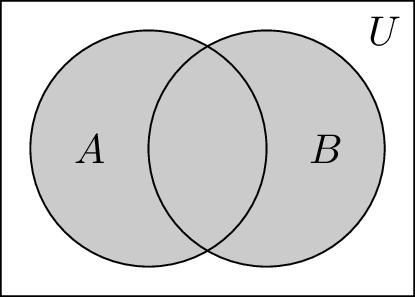
\includegraphics{./tikz/union.png}

}

\caption{Union}

}

\end{minipage}%
%
\begin{minipage}[t]{0.50\linewidth}

{\centering 

\raisebox{-\height}{

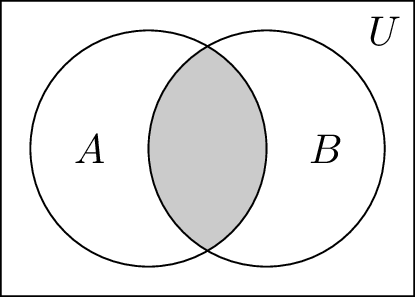
\includegraphics{./tikz/intersection.png}

}

\caption{Intersection}

}

\end{minipage}%
\newline
\begin{minipage}[t]{0.50\linewidth}

{\centering 

\raisebox{-\height}{

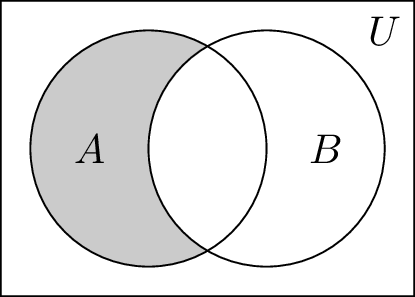
\includegraphics{./tikz/difference.png}

}

\caption{Différence}

}

\end{minipage}%
%
\begin{minipage}[t]{0.50\linewidth}

{\centering 

\raisebox{-\height}{

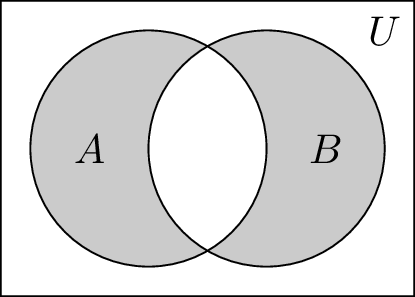
\includegraphics{./tikz/difference_symetrique.png}

}

\caption{Différence symétrique}

}

\end{minipage}%
\newline
\begin{minipage}[t]{0.50\linewidth}

{\centering 

\raisebox{-\height}{

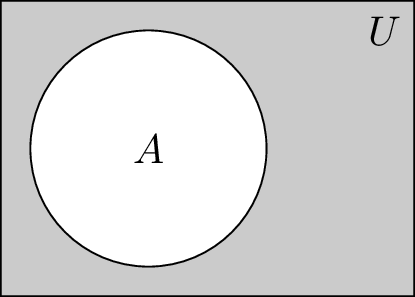
\includegraphics{./tikz/complement.png}

}

\caption{Complément}

}

\end{minipage}%

\end{figure}

Vous pouvez effectuer ces opérations dans \texttt{Python} à l'aide des
commandes suivantes:

\hypertarget{tbl-operations-ensembles-python}{}
\begin{longtable}[]{@{}ll@{}}
\caption{\label{tbl-operations-ensembles-python}Les opérations sur les
ensembles dans \texttt{Python}.}\tabularnewline
\toprule()
\textbf{Opération} & \textbf{Commande} \texttt{Python} \\
\midrule()
\endfirsthead
\toprule()
\textbf{Opération} & \textbf{Commande} \texttt{Python} \\
\midrule()
\endhead
\textbf{Union} & \texttt{union} \\
\textbf{Intersection} & \texttt{intersection} \\
\textbf{Différence} & \texttt{difference} \\
\bottomrule()
\end{longtable}

\hypertarget{union-python}{}
\begin{Shaded}
\begin{Highlighting}[]
\NormalTok{A }\OperatorTok{=}\NormalTok{ \{}\OperatorTok{{-}}\DecValTok{3}\NormalTok{,}\OperatorTok{{-}}\DecValTok{1}\NormalTok{,}\DecValTok{2}\NormalTok{,}\DecValTok{5}\NormalTok{\}}
\NormalTok{B }\OperatorTok{=}\NormalTok{ \{}\OperatorTok{{-}}\DecValTok{1}\NormalTok{, }\DecValTok{0}\NormalTok{, }\DecValTok{2}\NormalTok{\}}
\BuiltInTok{print}\NormalTok{(A.union(B))}
\end{Highlighting}
\end{Shaded}

\begin{verbatim}
{0, 2, 5, -3, -1}
\end{verbatim}

\hypertarget{intersection-python}{}
\begin{Shaded}
\begin{Highlighting}[]
\NormalTok{A }\OperatorTok{=}\NormalTok{ \{}\OperatorTok{{-}}\DecValTok{3}\NormalTok{,}\OperatorTok{{-}}\DecValTok{1}\NormalTok{,}\DecValTok{2}\NormalTok{,}\DecValTok{5}\NormalTok{\}}
\NormalTok{B }\OperatorTok{=}\NormalTok{ \{}\OperatorTok{{-}}\DecValTok{1}\NormalTok{, }\DecValTok{0}\NormalTok{, }\DecValTok{2}\NormalTok{\}}
\BuiltInTok{print}\NormalTok{(A.intersection(B))}
\end{Highlighting}
\end{Shaded}

\begin{verbatim}
{2, -1}
\end{verbatim}

\hypertarget{difference-python}{}
\begin{Shaded}
\begin{Highlighting}[]
\NormalTok{A }\OperatorTok{=}\NormalTok{ \{}\OperatorTok{{-}}\DecValTok{3}\NormalTok{,}\OperatorTok{{-}}\DecValTok{1}\NormalTok{,}\DecValTok{2}\NormalTok{,}\DecValTok{5}\NormalTok{\}}
\NormalTok{B }\OperatorTok{=}\NormalTok{ \{}\OperatorTok{{-}}\DecValTok{1}\NormalTok{, }\DecValTok{0}\NormalTok{, }\DecValTok{2}\NormalTok{\}}
\BuiltInTok{print}\NormalTok{(A.difference(B))}
\end{Highlighting}
\end{Shaded}

\begin{verbatim}
{5, -3}
\end{verbatim}

\hypertarget{repruxe9sentation-de-sous-ensembles-par-trains-de-bits}{%
\section{Représentation de sous-ensembles par trains de
bits}\label{repruxe9sentation-de-sous-ensembles-par-trains-de-bits}}

\hypertarget{polygones-convexes-avec-des-opuxe9rations-sur-les-ensembles}{%
\section{Polygones convexes avec des opérations sur les
ensembles}\label{polygones-convexes-avec-des-opuxe9rations-sur-les-ensembles}}

\bookmarksetup{startatroot}

\hypertarget{fonctions}{%
\chapter{Fonctions}\label{fonctions}}

\leavevmode\vadjust pre{\hypertarget{def-fonction}{}}%
\begin{definition}[Fonction]\label{def-fonction}

Une \textbf{fonction} \(f\) d'un ensemble \(A\) vers un ensemble \(B\)
est une règle qui, à chaque élément \(a\) de l'ensemble \(A\), associe
un et un seul élément \(b\) de l'ensemble \(B\). Cet élément \(b\) est
noté \(f(a)\). On écrit parfois \((a,b)\in f\).

La notation usuelle pour désigner une fonction \(f\) d'un ensemble \(A\)
vers un ensemble \(B\) est \[
f:A\rightarrow B
\] L'ensemble \(A\) est appelé le \textbf{domaine} de la fonction \(f\),
noté \(\mathbf{dom} (f)\), et le sous-ensemble \(B\) formé des éléments
atteints par \(f\) est appelé l'\textbf{image} de \(f\), noté
\(\mathbf{ima} (f)\). \[
\mathbf{ima} (f) = \set{b\in B\ \mid\ \exists a\in A,\ f(a)=b} \subseteq B
\]

\end{definition}

Par ailleurs, on peut aussi voir une fonction \(f\) de \(A\) vers \(B\)
comme un sous-ensemble du produit cartésien \(A\times B\) ayant la
propriété suivante: \[
\forall\ a\in A,\ \exists !b\in B,\ (a,b)\in f
\] où le symbole \(\exists !\) désigne \textbf{il existe un et un seul}.

\leavevmode\vadjust pre{\hypertarget{exm-fonction-trains-bits-longueur-8}{}}%
\begin{example}[]\label{exm-fonction-trains-bits-longueur-8}

Considérons \(T_8\), l'ensemble des trains de bits de longueur 8 et la
fonction \(f:T_8\rightarrow \mathbb{N}\) définie par \[
f(t)=\text{nombre de 0 dans le train de bits}\ t
\] Par exemple, \(f(1100\ 1011)=3\). Donnez le domaine et l'image de la
fonction \(f\).

\end{example}

\hypertarget{fonctions-plancher-et-plafond}{%
\section{Fonctions plancher et
plafond}\label{fonctions-plancher-et-plafond}}

\leavevmode\vadjust pre{\hypertarget{def-fonction-plancher-plafond}{}}%
\begin{definition}[Fonctions plancher et
plafond]\label{def-fonction-plancher-plafond}

La fonction \textbf{plancher} associe à tout nombre réel \(x\), le plus
grand entier \(n\) tel que \(n\leq x\). On note
\(\lfloor x\rfloor = n\). La fonction \textbf{plafond} associe à tout
nombre réel \(x\), le plus petit entier \(n\) tel que \(n\geq x\). On
note \(\lceil x \rceil = n\).

\end{definition}

\leavevmode\vadjust pre{\hypertarget{exm-fonction-plancher-et-plafond}{}}%
\begin{example}[]\label{exm-fonction-plancher-et-plafond}

Calculez les fonctions suivantes: \begin{align*}
\left\lfloor \frac{1}{3}\right\rfloor &= \\
\left\lceil \frac{1}{3}\right\rceil &= \\
\left\lfloor -9,2\right\rfloor &= \\
\left\lceil -9,2\right\rceil &= \\
\end{align*}

\end{example}

\leavevmode\vadjust pre{\hypertarget{thm-proprietes-plancher-plafond}{}}%
\begin{theorem}[Propriétés des fonctions plancher et
plafond]\label{thm-proprietes-plancher-plafond}

~

\begin{enumerate}
\def\labelenumi{\arabic{enumi}.}
\tightlist
\item
  \(\lfloor x\rfloor = n\) \(\leftrightarrow\) \(n\leq x<n+1\)
\item
  \(\lceil x\rceil = n\) \(\leftrightarrow\) \(n-1< x\leq n\)
\item
  \(x-1<\lfloor x\rfloor \leq x \leq \lceil x \rceil < x+1\)
\end{enumerate}

\end{theorem}

La Figure~\ref{fig-floor-ceiling} présente le graphique des fonctions
plancher et plafond.

\begin{figure}

\begin{minipage}[t]{0.50\linewidth}

{\centering 

\raisebox{-\height}{

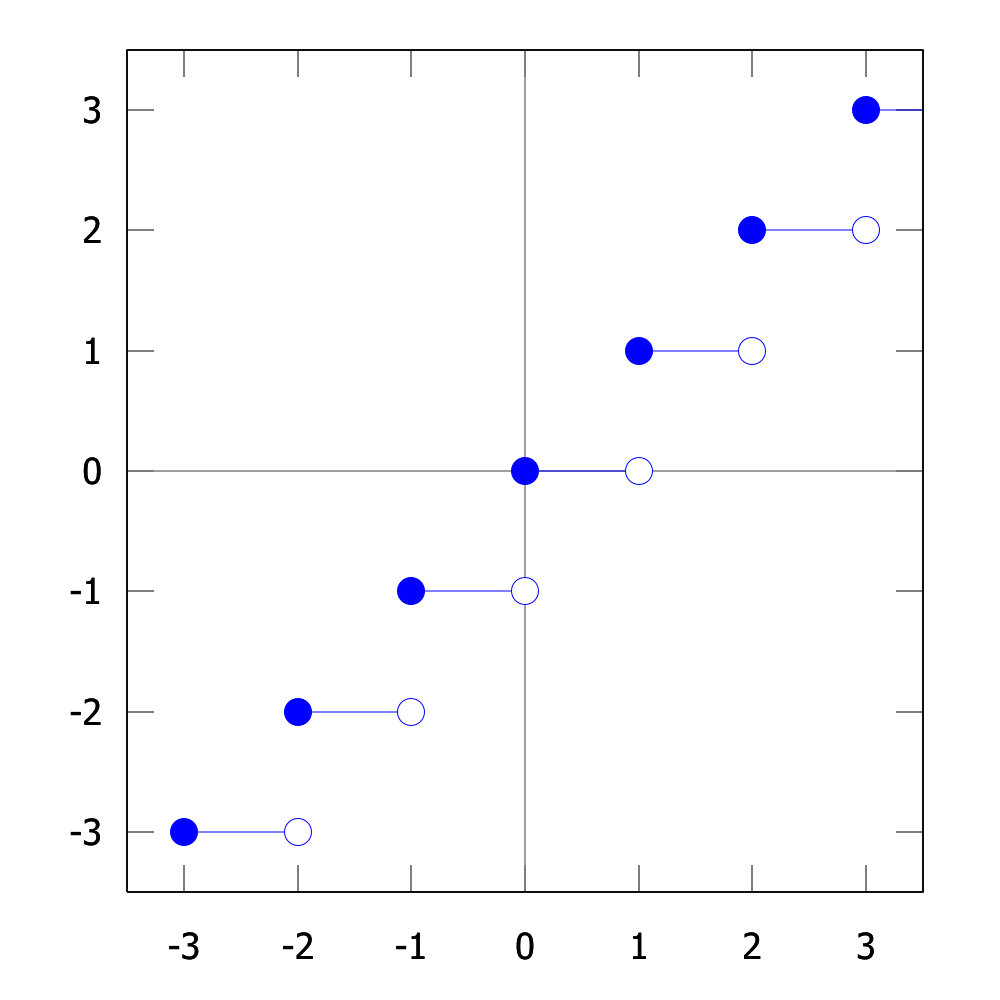
\includegraphics{./figs/floor_function.png}

}

\caption{Fonction plancher}

}

\end{minipage}%
%
\begin{minipage}[t]{0.50\linewidth}

{\centering 

\raisebox{-\height}{

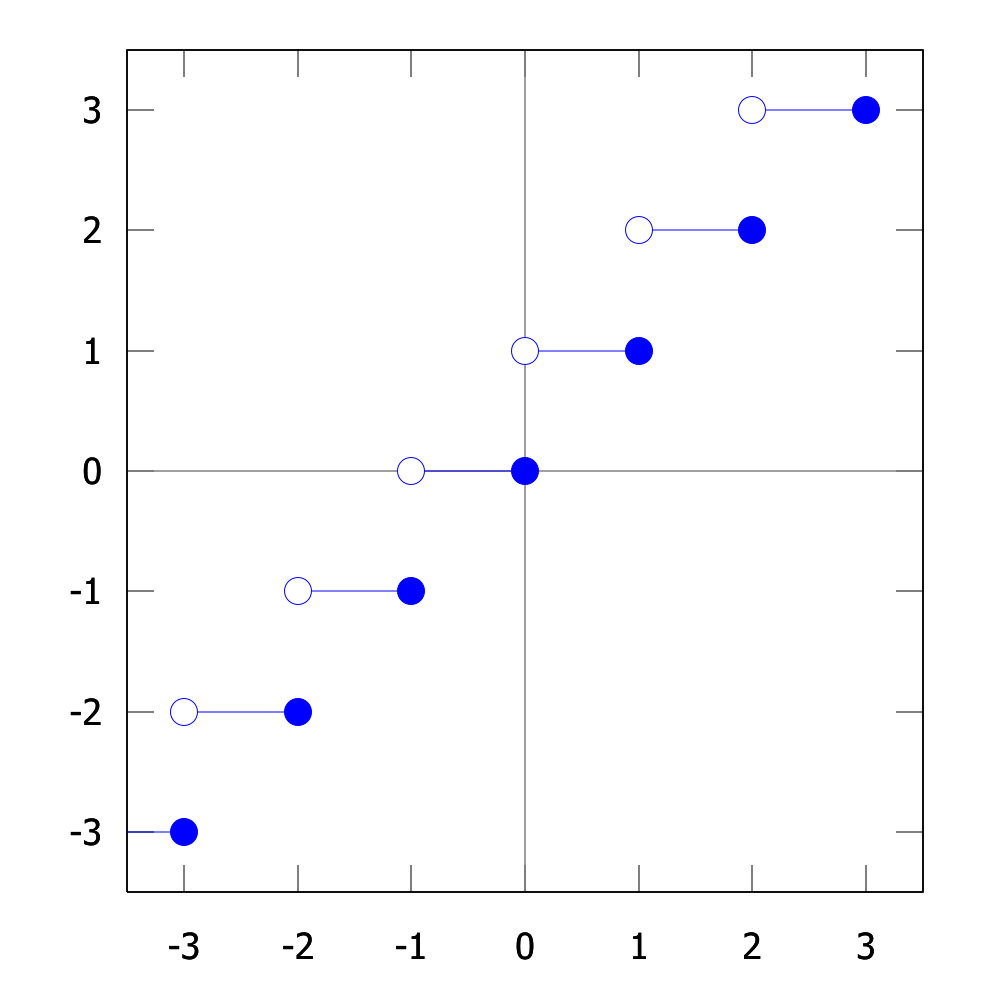
\includegraphics{./figs/ceiling_function.png}

}

\caption{Fonction plafond}

}

\end{minipage}%

\caption{\label{fig-floor-ceiling}Les fonctions plancher et plafond.}

\end{figure}

Ces deux fonctions sont accessibles dans \texttt{Python} en utilisant la
librairie \texttt{math}, sous le nom de \texttt{floor} (\emph{fonction
plancher}) et \texttt{ceil} (\emph{fonction plafond}).

\hypertarget{fonctions-planchers-plafonds}{}
\begin{Shaded}
\begin{Highlighting}[]
\ImportTok{import}\NormalTok{ math}

\BuiltInTok{print}\NormalTok{(}\StringTok{"Résultats de la fonction plafond"}\NormalTok{)}
\BuiltInTok{print}\NormalTok{(math.ceil(}\FloatTok{1.4}\NormalTok{))}
\BuiltInTok{print}\NormalTok{(math.ceil(}\FloatTok{5.3}\NormalTok{))}
\BuiltInTok{print}\NormalTok{(math.ceil(}\OperatorTok{{-}}\FloatTok{5.3}\NormalTok{))}
\BuiltInTok{print}\NormalTok{(math.ceil(}\FloatTok{22.6}\NormalTok{))}
\BuiltInTok{print}\NormalTok{(math.ceil(}\FloatTok{10.0}\NormalTok{))}

\BuiltInTok{print}\NormalTok{(}\StringTok{"Résultats de la fonction plancher"}\NormalTok{)}
\BuiltInTok{print}\NormalTok{(math.floor(}\FloatTok{1.4}\NormalTok{))}
\BuiltInTok{print}\NormalTok{(math.floor(}\FloatTok{5.3}\NormalTok{))}
\BuiltInTok{print}\NormalTok{(math.floor(}\OperatorTok{{-}}\FloatTok{5.3}\NormalTok{))}
\BuiltInTok{print}\NormalTok{(math.floor(}\FloatTok{22.6}\NormalTok{))}
\BuiltInTok{print}\NormalTok{(math.floor(}\FloatTok{10.0}\NormalTok{))}
\end{Highlighting}
\end{Shaded}

\begin{verbatim}
Résultats de la fonction plafond
2
6
-5
23
10
Résultats de la fonction plancher
1
5
-6
22
10
\end{verbatim}

\hypertarget{fonctions-en-python}{%
\section{\texorpdfstring{Fonctions en
\texttt{Python}}{Fonctions en Python}}\label{fonctions-en-python}}

DEVRAIT-ON PARLER DE ÇA????

DICTIONNAIRE, HACHAGE\ldots{}

\leavevmode\vadjust pre{\hypertarget{exm-hash-python}{}}%
\begin{example}[]\label{exm-hash-python}

\href{https://www.wikiwand.com/en/Fowler\%E2\%80\%93Noll\%E2\%80\%93Vo_hash_function}{Fonction
de hachage dans Python}

\href{https://andrewbrookins.com/technology/pythons-default-hash-algorithm/}{Hachage
Python}

\href{https://thepythoncorner.com/posts/2020-08-21-hash-tables-understanding-dictionaries/}{Dictionnary
in Python}

A checksum is used to determine if something is the same.

If you have download a file, you can never be sure if it got corrupted
on the way to your machine. You can use cksum to calculate a checksum
(based on CRC-32) of the copy you now have and can then compare it to
the checksum the file should have. This is how you check for file
integrity.

A hash function is used to map data to other data of fixed size. A
perfect hash function is injective, so there are no collisions. Every
input has one fixed output.

A cryptographic hash function is used for verification. With a
cryptographic hash function you should to not be able to compute the
original input.

A very common use case is password hashing. This allows the verification
of a password without having to save the password itself. A service
provider only saves a hash of a password and is not able to compute the
original password. If the database of password hashes gets compromised,
an attacker should not be able to compute these passwords as well. This
is not the case, because there are strong and weak algorithms for
password hashing. You can find more on that on this very site.

TL;DR:

Checksums are used to compare two pieces of information to check if two
parties have exactly the same thing.

Hashes are used (in cryptography) to verify something, but this time,
deliberately only one party has access to the data that has to be
verified, while the other party only has access to the hash.

\end{example}

\hypertarget{injection-surjection-et-bijection}{%
\section{Injection, surjection et
bijection}\label{injection-surjection-et-bijection}}

\leavevmode\vadjust pre{\hypertarget{def-fonction-injective-surjective-bijective}{}}%
\begin{definition}[Fonction injective, surjective,
bijective]\label{def-fonction-injective-surjective-bijective}

Soit \(f:A\rightarrow B\) une fonction. On dit que

\begin{itemize}
\tightlist
\item
  \textbf{\(f\) est injective} si elle n'associe jamais la même image à
  deux éléments distincts: \[
  \forall\ a_1 \in A,\ \forall\ a_2 \in A,\ (a_1\neq a_2) \rightarrow (f(a_1) \neq f(a_2))
  \]
\item
  \textbf{\(f\) est surjective} si son image est l'ensemble \(B\) au
  complet, c'est-à-dire si tous les éléments de \(B\) sont atteints: \[
  \forall\ b\in B,\ \exists\ a \in A,\ f(a)=b
  \]
\item
  \textbf{\(f\) est bijective} si elle est injective et surjective: \[
  \forall\ b\in B,\ \exists! a\in A,\ f(a)=b
  \]
\end{itemize}

\end{definition}

\begin{tcolorbox}[enhanced jigsaw, opacityback=0, rightrule=.15mm, breakable, toprule=.15mm, colbacktitle=quarto-callout-important-color!10!white, title=\textcolor{quarto-callout-important-color}{\faExclamation}\hspace{0.5em}{Important}, titlerule=0mm, arc=.35mm, colback=white, coltitle=black, colframe=quarto-callout-important-color-frame, bottomtitle=1mm, toptitle=1mm, bottomrule=.15mm, leftrule=.75mm, left=2mm, opacitybacktitle=0.6]

Si une fonction n'est pas \textbf{injective}, alors elle ne possède pas
d'inverse.

\end{tcolorbox}

\begin{tcolorbox}[enhanced jigsaw, opacityback=0, rightrule=.15mm, breakable, toprule=.15mm, colbacktitle=quarto-callout-important-color!10!white, title=\textcolor{quarto-callout-important-color}{\faExclamation}\hspace{0.5em}{Important}, titlerule=0mm, arc=.35mm, colback=white, coltitle=black, colframe=quarto-callout-important-color-frame, bottomtitle=1mm, toptitle=1mm, bottomrule=.15mm, leftrule=.75mm, left=2mm, opacitybacktitle=0.6]

Si une fonction n'est pas \textbf{surjective}, alors elle ne possède pas
d'inverse.

\end{tcolorbox}

\leavevmode\vadjust pre{\hypertarget{exm-fonction-injective-surjective-bijective}{}}%
\begin{example}[]\label{exm-fonction-injective-surjective-bijective}

On considère un sous-ensemble \(f\) du produit cartésien de deux
ensembles. Dans chaque cas, tracez son graphe saggital puis déterminez
s'il s'agit d'une fonction ou non. De plus, si \(f\) est une fonction,
déterminez si elle est injective, surjective ou bijective.

Ici, \(L=\set{a,b,c,d,e}\), \(M=\set{a,b,c}\), \(C=\set{1,2,3,4}\) et
\(D=\set{1,2,3}\).

\begin{enumerate}
\def\labelenumi{\alph{enumi}.}
\tightlist
\item
  \(f=\set{(1,a),(2,d),(3,c),(4,e)}\subseteq C \times L\)
\item
  \(f=\set{(1,a),(2,a),(3,c),(4,b)}\subseteq C \times M\)
\item
  \(f=\set{(1,a),(2,d),(3,c),(4,e),(1,b)}\subseteq C \times L\)
\item
  \(f=\set{(1,c),(2,a),(3,a),(4,a)}\subseteq D \times M\)
\item
  \(f=\set{(1,a),(2,a),(3,a),(4,a)}\subseteq C \times L\)
\end{enumerate}

\end{example}

\leavevmode\vadjust pre{\hypertarget{exm-fonction-dans-Z}{}}%
\begin{example}[]\label{exm-fonction-dans-Z}

La fonction \(f:\mathbb{Z}\times\mathbb{Z}\rightarrow \mathbb{Z}\)
définie par \(f(x_1,x_2)=x_1+x^2\) est-elle oui on non injective?
Est-elle oui ou non surjective? Est-elle oui ou non bijective?

\end{example}

\hypertarget{les-dictionnaires-dans-python}{%
\subsection{\texorpdfstring{Les dictionnaires dans
\texttt{Python}}{Les dictionnaires dans Python}}\label{les-dictionnaires-dans-python}}

Le dictionnaire n'est pas une séquence mais un autre type composite. Ils
ressemblent aux listes dans une certaine mesure (ils sont modifiables
comme elles), mais les éléments que nous allons y enregistrer ne seront
pas disposés dans un ordre immuable. En revanche, nous pourrons accéder
à n'importe lequel d'entre eux à l'aide d'un index spécifique que l'on
appellera une clé, laquelle pourra être alphabétique, numérique, ou même
d'un type composite sous certaines conditions.

\leavevmode\vadjust pre{\hypertarget{exm-jour-dejeuner-injective}{}}%
\begin{example}[]\label{exm-jour-dejeuner-injective}

Dites si le dictionnaire défini ci-dessous est une fonction injective,
surjective, ou bijective.

\hypertarget{dictionnaries-days-breakfast-injective}{}
\begin{Shaded}
\begin{Highlighting}[]
\NormalTok{jour }\OperatorTok{=}\NormalTok{ \{}\StringTok{"Lundi"}\NormalTok{, }\StringTok{"Mardi"}\NormalTok{, }\StringTok{"Mercredi"}\NormalTok{, }\StringTok{"Jeudi"}\NormalTok{, }\StringTok{"Vendredi"}\NormalTok{, }\StringTok{"Samedi"}\NormalTok{, }\StringTok{"Dimanche"}\NormalTok{\}}
\NormalTok{dejeuner }\OperatorTok{=}\NormalTok{ \{}\StringTok{"Oeufs"}\NormalTok{, }\StringTok{"Céréales"}\NormalTok{, }\StringTok{"Rôties"}\NormalTok{, }\StringTok{"Gruau"}\NormalTok{, }\StringTok{"Pâtisserie"}\NormalTok{, }\StringTok{"Jambon"}\NormalTok{, }\StringTok{"Crèpes"}\NormalTok{,}\StringTok{"Saucisses"}\NormalTok{\}}

\NormalTok{mydict }\OperatorTok{=}\NormalTok{ \{}
    \StringTok{"Lundi"}\NormalTok{: }\StringTok{"Oeufs"}\NormalTok{,}
    \StringTok{"Mardi"}\NormalTok{: }\StringTok{"Céréales"}\NormalTok{,}
    \StringTok{"Mercredi"}\NormalTok{: }\StringTok{"Rôties"}\NormalTok{,}
    \StringTok{"Jeudi"}\NormalTok{: }\StringTok{"Gruau"}\NormalTok{,}
    \StringTok{"Vendredi"}\NormalTok{: }\StringTok{"Pâtisserie"}\NormalTok{,}
    \StringTok{"Samedi"}\NormalTok{: }\StringTok{"Jambon"}\NormalTok{,}
    \StringTok{"Dimanche"}\NormalTok{: }\StringTok{"Crèpes"}
\NormalTok{\}}
\end{Highlighting}
\end{Shaded}

\end{example}

\leavevmode\vadjust pre{\hypertarget{exm-jour-dejeuner-non-injective}{}}%
\begin{example}[]\label{exm-jour-dejeuner-non-injective}

Dites si le dictionnaire défini ci-dessous est une fonction injective,
surjective, ou bijective.

\hypertarget{dictionnaries-days-breakfast-non-injective}{}
\begin{Shaded}
\begin{Highlighting}[]
\NormalTok{jour }\OperatorTok{=}\NormalTok{ \{}\StringTok{"Lundi"}\NormalTok{, }\StringTok{"Mardi"}\NormalTok{, }\StringTok{"Mercredi"}\NormalTok{, }\StringTok{"Jeudi"}\NormalTok{, }\StringTok{"Vendredi"}\NormalTok{, }\StringTok{"Samedi"}\NormalTok{, }\StringTok{"Dimanche"}\NormalTok{\}}
\NormalTok{dejeuner }\OperatorTok{=}\NormalTok{ \{}\StringTok{"Oeufs"}\NormalTok{, }\StringTok{"Céréales"}\NormalTok{, }\StringTok{"Rôties"}\NormalTok{, }\StringTok{"Gruau"}\NormalTok{, }\StringTok{"Pâtisserie"}\NormalTok{, }\StringTok{"Jambon"}\NormalTok{, }\StringTok{"Crèpes"}\NormalTok{,}\StringTok{"Saucisses"}\NormalTok{\}}

\NormalTok{mydict }\OperatorTok{=}\NormalTok{ \{}
    \StringTok{"Lundi"}\NormalTok{: }\StringTok{"Oeufs"}\NormalTok{,}
    \StringTok{"Mardi"}\NormalTok{: }\StringTok{"Oeufs"}\NormalTok{,}
    \StringTok{"Mercredi"}\NormalTok{: }\StringTok{"Rôties"}\NormalTok{,}
    \StringTok{"Jeudi"}\NormalTok{: }\StringTok{"Gruau"}\NormalTok{,}
    \StringTok{"Vendredi"}\NormalTok{: }\StringTok{"Pâtisserie"}\NormalTok{,}
    \StringTok{"Samedi"}\NormalTok{: }\StringTok{"Jambon"}\NormalTok{,}
    \StringTok{"Dimanche"}\NormalTok{: }\StringTok{"Crèpes"}
\NormalTok{\}}
\end{Highlighting}
\end{Shaded}

\end{example}

\hypertarget{fonction-de-hachage}{%
\subsection{Fonction de hachage}\label{fonction-de-hachage}}

Une \textbf{fonction de hachage} est une fonction qui associe des
données de taille arbitraire à des valeurs de taille fixe. Les valeurs
renvoyées par une fonction de hachage sont appelées valeurs de hachage,
codes de hachage, résumés, signatures ou simplement hachages. Les
valeurs sont généralement utilisées pour être les indices d'une table de
taille raisonnable appelée table de hachage. Le hachage ou adressage de
stockage dispersé est donc l'utilisation d'une fonction de hachage pour
créer les indices d'une table de hachage.

Les fonctions de hachage sont utilisées dans les applications de
stockage et de récupération de données pour accéder aux données en un
temps réduit, en fait quasi-constant. Elles requièrent un espace de
stockage à peine plus grand que l'espace total requis pour les données.
Ainsi, le hachage est une forme d'accès aux données efficace en termes
de calcul et d'espace de stockage.

L'intérêt des fonctions de hachage repose sur de bonnes propriétés
statistiques. En effet, le comportement dans le pire des cas est
mauvais, mais il se manifeste avec une probabilité extrêmement faible,
en fait négligeable, et le comportement dans le cas moyen est optimal
(collision minimale ).

Une fonction de hachage est typiquement une fonction qui, pour un
ensemble de très grande taille (théoriquement infini) et de nature très
diversifiée, va renvoyer des résultats aux spécifications précises (en
général des chaînes de caractère de taille limitée ou fixe) optimisées
pour des applications particulières. Les chaînes permettent d'établir
des relations (égalité, égalité probable, non-égalité, ordre\ldots)
entre les objets de départ sans accéder directement à ces derniers, en
général soit pour des questions d'optimisation (la taille des objets de
départ nuit aux performances), soit pour des questions de
confidentialité.

Autrement dit : à 1 fichier (ou à 1 mot) va correspondre une signature
unique (le résultat de la fonction de hachage).

\begin{tcolorbox}[enhanced jigsaw, opacityback=0, rightrule=.15mm, breakable, toprule=.15mm, colbacktitle=quarto-callout-important-color!10!white, title=\textcolor{quarto-callout-important-color}{\faExclamation}\hspace{0.5em}{Important}, titlerule=0mm, arc=.35mm, colback=white, coltitle=black, colframe=quarto-callout-important-color-frame, bottomtitle=1mm, toptitle=1mm, bottomrule=.15mm, leftrule=.75mm, left=2mm, opacitybacktitle=0.6]

Dans l'idéal, une fonction de hachage \emph{devrait} être injective.

\end{tcolorbox}

On peut trouver le haché d'un élément en \texttt{Python} en utilisant la
commande \texttt{hash}. On peut remarquer dans le code ci-dessous que de
changer une lettre minuscule en lettre majuscule (le \emph{F} de
fromage) change drastiquement le haché.

\hypertarget{fonction-hachage-renard-corbeau}{}
\begin{Shaded}
\begin{Highlighting}[]
\NormalTok{phrase1 }\OperatorTok{=} \StringTok{"Maître Corbeau, sur un arbre perché, Tenait en son bec un fromage."}
\NormalTok{phrase2 }\OperatorTok{=} \StringTok{"Maître Corbeau, sur un arbre perché, Tenait en son bec un Fromage."}

\BuiltInTok{print}\NormalTok{(}\BuiltInTok{hex}\NormalTok{(}\BuiltInTok{hash}\NormalTok{(phrase1)), }\BuiltInTok{hex}\NormalTok{(}\BuiltInTok{hash}\NormalTok{(phrase2)))}
\end{Highlighting}
\end{Shaded}

\begin{verbatim}
-0x30c2cc09142bd723 0x2881da047751f3c2
\end{verbatim}

\bookmarksetup{startatroot}

\hypertarget{notation-grand-o}{%
\chapter{Notation grand O}\label{notation-grand-o}}

\hypertarget{mesurer-un-temps-de-calcul-avec-une-fonction}{%
\section{Mesurer un temps de calcul avec une
fonction}\label{mesurer-un-temps-de-calcul-avec-une-fonction}}

\hypertarget{notation-grand-o-1}{%
\section{Notation grand-O}\label{notation-grand-o-1}}

\hypertarget{sommations}{%
\section{Sommations}\label{sommations}}

\hypertarget{uxe9tablir-la-complexituxe9-dun-algorithme}{%
\section{Établir la complexité d'un
algorithme}\label{uxe9tablir-la-complexituxe9-dun-algorithme}}

\hypertarget{calculabilituxe9-et-complexituxe9}{%
\section{Calculabilité et
complexité}\label{calculabilituxe9-et-complexituxe9}}

\hypertarget{p-vs-np}{%
\section{P vs NP}\label{p-vs-np}}

\bookmarksetup{startatroot}

\hypertarget{introduction-aux-algorithmes}{%
\chapter{Introduction aux
algorithmes}\label{introduction-aux-algorithmes}}

\hypertarget{bogo-sort}{%
\section{Bogo sort}\label{bogo-sort}}

\begin{Shaded}
\begin{Highlighting}[]
\ImportTok{from}\NormalTok{ random }\ImportTok{import}\NormalTok{ shuffle}
\ImportTok{from}\NormalTok{ random }\ImportTok{import}\NormalTok{ seed}
\ImportTok{from}\NormalTok{ random }\ImportTok{import}\NormalTok{ randint}

\KeywordTok{def}\NormalTok{ is\_sorted(data) }\OperatorTok{{-}\textgreater{}} \BuiltInTok{bool}\NormalTok{:}
    \CommentTok{"""Determine whether the data is sorted."""}
    \ControlFlowTok{return} \BuiltInTok{all}\NormalTok{(a }\OperatorTok{\textless{}=}\NormalTok{ b }\ControlFlowTok{for}\NormalTok{ a, b }\KeywordTok{in} \BuiltInTok{zip}\NormalTok{(data, data[}\DecValTok{1}\NormalTok{:]))}

\KeywordTok{def}\NormalTok{ bogosort(data) }\OperatorTok{{-}\textgreater{}} \BuiltInTok{list}\NormalTok{:}
    \CommentTok{"""Shuffle data until sorted."""}
\NormalTok{    N }\OperatorTok{=} \DecValTok{0}
    \ControlFlowTok{while} \KeywordTok{not}\NormalTok{ is\_sorted(data):}
\NormalTok{        shuffle(data)}
\NormalTok{        N }\OperatorTok{=}\NormalTok{ N }\OperatorTok{+} \DecValTok{1}
    \ControlFlowTok{return}\NormalTok{ data, N}

\NormalTok{seed(}\DecValTok{1234}\NormalTok{)}
\NormalTok{N }\OperatorTok{=} \DecValTok{8}
\NormalTok{data }\OperatorTok{=}\NormalTok{ [randint(}\DecValTok{1}\NormalTok{,}\DecValTok{10}\NormalTok{) }\ControlFlowTok{for}\NormalTok{ x }\KeywordTok{in} \BuiltInTok{range}\NormalTok{(N)]}
\NormalTok{bogosort(data)}
\end{Highlighting}
\end{Shaded}

\begin{verbatim}
([1, 1, 2, 2, 2, 2, 8, 10], 1552)
\end{verbatim}

\hypertarget{exemples-dalgorithmes}{%
\section{Exemples d'algorithmes}\label{exemples-dalgorithmes}}

\hypertarget{fouille-linuxe9aire}{%
\section{Fouille linéaire}\label{fouille-linuxe9aire}}

\hypertarget{bubble-sort}{%
\section{Bubble sort}\label{bubble-sort}}

\hypertarget{insertion-sort}{%
\section{Insertion sort}\label{insertion-sort}}

\hypertarget{binary-search}{%
\section{Binary search}\label{binary-search}}

\hypertarget{heap-sort}{%
\section{Heap sort}\label{heap-sort}}

\hypertarget{complexituxe9-algorithmique}{%
\section{Complexité algorithmique}\label{complexituxe9-algorithmique}}

\bookmarksetup{startatroot}

\hypertarget{thuxe9orie-des-nombres}{%
\chapter{Théorie des nombres}\label{thuxe9orie-des-nombres}}

\hypertarget{arithmuxe9tique-modulaire}{%
\section{Arithmétique modulaire}\label{arithmuxe9tique-modulaire}}

\hypertarget{division-entiuxe8re-1}{%
\subsection{Division entière}\label{division-entiuxe8re-1}}

\hypertarget{congruence-modulo-m}{%
\subsection{\texorpdfstring{Congruence modulo
\(m\)}{Congruence modulo m}}\label{congruence-modulo-m}}

\hypertarget{entiers-et-algorithmes}{%
\section{Entiers et algorithmes}\label{entiers-et-algorithmes}}

\hypertarget{algorithme-dexponentiation-modulaire-efficace}{%
\subsection{Algorithme d'exponentiation modulaire
efficace}\label{algorithme-dexponentiation-modulaire-efficace}}

\hypertarget{nombres-premiers-et-pgcd}{%
\subsection{Nombres premiers et PGCD}\label{nombres-premiers-et-pgcd}}

\hypertarget{algorithme-deuclide-et-thuxe9oruxe8me-de-buxe9zout}{%
\subsection{Algorithme d'Euclide et théorème de
Bézout}\label{algorithme-deuclide-et-thuxe9oruxe8me-de-buxe9zout}}

\hypertarget{inverse-modulo-m}{%
\subsection{\texorpdfstring{Inverse modulo
\(m\)}{Inverse modulo m}}\label{inverse-modulo-m}}

\hypertarget{ruxe9solution-de-congruence}{%
\subsection{Résolution de
congruence}\label{ruxe9solution-de-congruence}}

\hypertarget{petit-thuxe9oruxe8me-de-fermat}{%
\subsection{Petit théorème de
Fermat}\label{petit-thuxe9oruxe8me-de-fermat}}

\hypertarget{cryptographie-uxe0-cluxe9-secruxe8te}{%
\section{Cryptographie à clé
secrète}\label{cryptographie-uxe0-cluxe9-secruxe8te}}

\hypertarget{chiffrement-par-duxe9calage}{%
\subsection{Chiffrement par
décalage}\label{chiffrement-par-duxe9calage}}

\hypertarget{permutation-de-lalphabet}{%
\subsection{Permutation de l'alphabet}\label{permutation-de-lalphabet}}

\hypertarget{masque-jetable}{%
\subsection{Masque jetable}\label{masque-jetable}}

\hypertarget{chiffrement-affine}{%
\subsection{Chiffrement affine}\label{chiffrement-affine}}

\hypertarget{cryptographie-uxe0-cluxe9-publique}{%
\section{Cryptographie à clé
publique}\label{cryptographie-uxe0-cluxe9-publique}}

\hypertarget{chiffrement-rsa}{%
\subsection{Chiffrement RSA}\label{chiffrement-rsa}}

\bookmarksetup{startatroot}

\hypertarget{preuves-et-raisonnement-mathuxe9matique}{%
\chapter{Preuves et raisonnement
mathématique}\label{preuves-et-raisonnement-mathuxe9matique}}

\hypertarget{muxe9thodes-de-preuve}{%
\section{Méthodes de preuve}\label{muxe9thodes-de-preuve}}

\hypertarget{preuve-directe}{%
\subsection{Preuve directe}\label{preuve-directe}}

\leavevmode\vadjust pre{\hypertarget{exm-produit-nombres-pairs-impairs}{}}%
\begin{example}[]\label{exm-produit-nombres-pairs-impairs}

LE PRODUIT DE NOMBRES PAIRS ET IMPAIRS

\end{example}

\leavevmode\vadjust pre{\hypertarget{exm-racines-nombres-pairs}{}}%
\begin{example}[]\label{exm-racines-nombres-pairs}

RACINE DE NOMBRES PAIRS

\end{example}

\leavevmode\vadjust pre{\hypertarget{exm-n2-pair}{}}%
\begin{example}[]\label{exm-n2-pair}

PREUVE QUE \(n^2\) EST PAIR

\end{example}

\leavevmode\vadjust pre{\hypertarget{exm-a-divise-b-divise-c}{}}%
\begin{example}[]\label{exm-a-divise-b-divise-c}

Soit \(a\), \(b\) et \(c\) des entiers. Si \(a|b\) et \(b|c\) alors
\(a|c\).

\end{example}

\hypertarget{preuve-indirecte-par-contraposuxe9e}{%
\subsection{Preuve indirecte (par
contraposée)}\label{preuve-indirecte-par-contraposuxe9e}}

\leavevmode\vadjust pre{\hypertarget{exm-n2-pair-alors-n-pair}{}}%
\begin{example}[]\label{exm-n2-pair-alors-n-pair}

Montrez que si \(n^2\) est pair alors \(n\) est pair.

\end{example}

\leavevmode\vadjust pre{\hypertarget{exm-aplusb-impair-a-b-impair}{}}%
\begin{example}[]\label{exm-aplusb-impair-a-b-impair}

Montrez que si \(a+b\) est impair, alors \(a\) est impair ou \(b\) est
impair.

\end{example}

\leavevmode\vadjust pre{\hypertarget{exm-nombre-premier-impair}{}}%
\begin{example}[]\label{exm-nombre-premier-impair}

Soit \(p\) un nombre premier. Si \(p\neq 2\) alors \(p\) est impair.

\end{example}

\hypertarget{preuve-par-contradiction}{%
\subsection{Preuve par contradiction}\label{preuve-par-contradiction}}

\leavevmode\vadjust pre{\hypertarget{exm-plus-petit-nombre-rationnel}{}}%
\begin{example}[]\label{exm-plus-petit-nombre-rationnel}

EXISTE-T-IL UN PLUS PETIT NOMBRE RATIONNEL POSITIF?

\end{example}

\leavevmode\vadjust pre{\hypertarget{exm-sqrt2-irrationnel}{}}%
\begin{example}[]\label{exm-sqrt2-irrationnel}

PREUVE QUE \(\sqrt{2}\) EST IRRATIONNEL

\end{example}

\leavevmode\vadjust pre{\hypertarget{exm-infinite-nombres-premiers}{}}%
\begin{example}[]\label{exm-infinite-nombres-premiers}

PREUVE QUE QU'IL EXISTE UNE INFINITÉ DE NOMBRES PREMIERS

\end{example}

\leavevmode\vadjust pre{\hypertarget{exm-pas-entiers-equation}{}}%
\begin{example}[]\label{exm-pas-entiers-equation}

Il n'existe pas d'entiers \(x\) et \(y\) tels que \(x^2=4y+2\).

\end{example}

\hypertarget{principe-des-tiroirs-de-dirichlet}{%
\subsection{Principe des tiroirs de
Dirichlet}\label{principe-des-tiroirs-de-dirichlet}}

\leavevmode\vadjust pre{\hypertarget{exm-fonction-hachage}{}}%
\begin{example}[Fonction de hachage]\label{exm-fonction-hachage}

Une fonction de hachage est une fonction qui transforme une suite de
bits de longueur arbitraire en une chaîne de longueur fixe. Du fait
qu'il y a plus de chaînes possibles en entrée qu'en sortie découle par
le principe des tiroirs l'existence de collisions : plusieurs chaînes
distinctes ont le même haché. Rendre ces collisions difficiles à
déterminer efficacement est un enjeu important en cryptographie.

\end{example}

\hypertarget{principe-de-linduction}{%
\section{Principe de l'induction}\label{principe-de-linduction}}

\hypertarget{preuve-par-ruxe9currence}{%
\subsection{Preuve par récurrence}\label{preuve-par-ruxe9currence}}

\leavevmode\vadjust pre{\hypertarget{exm-somme-n-premiers-entiers}{}}%
\begin{example}[]\label{exm-somme-n-premiers-entiers}

PREUVE QUE \(1+2+3+\ldots +n=\frac{n(n+1)}{2}\)

\end{example}

\leavevmode\vadjust pre{\hypertarget{exm-n-plus-petit-2n}{}}%
\begin{example}[]\label{exm-n-plus-petit-2n}

PREUVE QUE \(n<2^n\)

\end{example}

\leavevmode\vadjust pre{\hypertarget{exm-6-divise-7n-1}{}}%
\begin{example}[]\label{exm-6-divise-7n-1}

PREUVE QUE 6 EST UN DIVISEUR DE \(7^n-1\)

\end{example}

\leavevmode\vadjust pre{\hypertarget{exm-space-filling-shapes}{}}%
\begin{example}[]\label{exm-space-filling-shapes}

MONTRER QUE NOUS POUVONS UTILISER DES T-GONES POUR REMPLIR UNE GRILLE
\(2^n \times 2^n\)

\end{example}

\leavevmode\vadjust pre{\hypertarget{exm-exponential-vs-factorial}{}}%
\begin{example}[]\label{exm-exponential-vs-factorial}

MONTRER QUE LA FACTORIELLE CROÎT PLUS RAPIDEMENT QUE L'EXPONENTIELLE

\end{example}

\hypertarget{algorithmes-ruxe9cursifs}{%
\subsection{Algorithmes récursifs}\label{algorithmes-ruxe9cursifs}}

\hypertarget{fonctions-ruxe9cursives}{%
\subsubsection{Fonctions récursives}\label{fonctions-ruxe9cursives}}

\hypertarget{algorithmes-de-type-diviser-pour-ruxe9gner}{%
\subsubsection{Algorithmes de type diviser pour
régner}\label{algorithmes-de-type-diviser-pour-ruxe9gner}}

\bookmarksetup{startatroot}

\hypertarget{duxe9nombrement}{%
\chapter{Dénombrement}\label{duxe9nombrement}}

\hypertarget{notions-de-base}{%
\section{Notions de base}\label{notions-de-base}}

\hypertarget{principe-des-nids-de-pigeon-principe-des-tiroirs-de-dirichlet}{%
\section{Principe des nids de pigeon (principe des tiroirs de
Dirichlet)}\label{principe-des-nids-de-pigeon-principe-des-tiroirs-de-dirichlet}}

\hypertarget{permutations-et-combinaisons}{%
\section{Permutations et
combinaisons}\label{permutations-et-combinaisons}}

\hypertarget{relations-de-ruxe9currence-et-duxe9nombrement}{%
\section{Relations de récurrence et
dénombrement}\label{relations-de-ruxe9currence-et-duxe9nombrement}}

\bookmarksetup{startatroot}

\hypertarget{graphes}{%
\chapter{Graphes}\label{graphes}}

\hypertarget{terminologie-et-types-de-graphes}{%
\section{Terminologie et types de
graphes}\label{terminologie-et-types-de-graphes}}

\hypertarget{repruxe9sentation-des-graphes}{%
\section{Représentation des
graphes}\label{repruxe9sentation-des-graphes}}

\hypertarget{repruxe9sentation-par-listes-dadjacence}{%
\subsection{Représentation par listes
d'adjacence}\label{repruxe9sentation-par-listes-dadjacence}}

\hypertarget{repruxe9sentation-par-matrice-dadjacence}{%
\subsection{Représentation par matrice
d'adjacence}\label{repruxe9sentation-par-matrice-dadjacence}}

\hypertarget{chemins-dans-un-graphe}{%
\section{Chemins dans un graphe}\label{chemins-dans-un-graphe}}

\hypertarget{chemins-circuits-cycles}{%
\subsection{Chemins, circuits, cycles}\label{chemins-circuits-cycles}}

\hypertarget{duxe9nombrement-de-chemins}{%
\subsection{Dénombrement de chemins}\label{duxe9nombrement-de-chemins}}

\hypertarget{chemins-et-circuits-euluxe9riens}{%
\subsection{Chemins et circuits
eulériens}\label{chemins-et-circuits-euluxe9riens}}

\hypertarget{chemins-et-circuits-hamiltoniens}{%
\subsection{Chemins et circuits
hamiltoniens}\label{chemins-et-circuits-hamiltoniens}}

\hypertarget{probluxe8me-du-plus-court-chemin}{%
\section{Problème du plus court
chemin}\label{probluxe8me-du-plus-court-chemin}}

\bookmarksetup{startatroot}

\hypertarget{arbres}{%
\chapter{Arbres}\label{arbres}}

\hypertarget{introduction-aux-arbres}{%
\section{Introduction aux arbres}\label{introduction-aux-arbres}}

\hypertarget{applications-des-arbres}{%
\section{Applications des arbres}\label{applications-des-arbres}}

\hypertarget{parcours-dun-arbre}{%
\section{Parcours d'un arbre}\label{parcours-dun-arbre}}

\hypertarget{arbres-et-tri}{%
\section{Arbres et tri}\label{arbres-et-tri}}

\hypertarget{arbres-et-recouvrement}{%
\section{Arbres et recouvrement}\label{arbres-et-recouvrement}}

\hypertarget{arbres-guxe9nuxe9rateurs-de-couxfbt-minimal}{%
\section{Arbres générateurs de coût
minimal}\label{arbres-guxe9nuxe9rateurs-de-couxfbt-minimal}}

\bookmarksetup{startatroot}

\hypertarget{ruxe9fuxe9rences}{%
\chapter*{Références}\label{ruxe9fuxe9rences}}
\addcontentsline{toc}{chapter}{Références}

\markboth{Références}{Références}

\hypertarget{refs}{}
\begin{CSLReferences}{0}{0}
\end{CSLReferences}


\backmatter

\end{document}
